 \documentclass{article}
\usepackage{tikz}
\usetikzlibrary{angles, quotes}
\usepackage{amssymb}
\usepackage{pgfplots}
\pgfplotsset{width=10cm,compat=1.9}
\usepgfplotslibrary{statistics}
\usepackage[left=2.54cm,right=2.54cm,top=2.54cm,bottom=2.54cm]{geometry}
\usepackage{tasks} %Paquete necesario para la producción de items horizontales para algunos ejercicios de tarea empleando el comando /begin{multicols}}{#}.../end{multicols} para ayudarnos a reducir las páginas
\usepackage{pdflscape} %comando que permite cambiar a orientación horizontal las hojas%
\usepackage{soul} %Paquete para permitir la compilación de acentos usando el comando {\hl{}}}\\
\sethlcolor{yellow(munsell)} %comando para definir el color para el subrayado usando el comando \hl
\usepackage[utf8]{inputenc}
\usepackage[spanish]{babel}
\usepackage{icomma}
\usepackage{ragged2e}
\usepackage{siunitx}
\usepackage{url}
\usepackage[colorlinks=true, urlcolor=blue,  linkcolor=black, citecolor=green]{hyperref}
\usepackage{pdfpages}
\usepackage{blindtext} %Paquete que genera texto ficticio (dummy text) con el comando: \blindtext
\usepackage{cancel} %in the preamble gives you four different modes of striking through: \cancel{text to cancel} draws a diagonal line (slash) through its argument, \bcancel{text to cancel} uses the negative slope (a backslash), \xcancel{text to cancel} draws an X (actually \cancel plus \bcancel), \cancelto{〈value〉}{〈expression〉} draws a diagonal arrow through the 〈expression〉pointing to the 〈value〉 (math-mode only)
\usepackage{csquotes}
\usepackage{afterpage}
\usepackage{parskip} 
\usepackage{float}
\usepackage{enumitem}
\usepackage{multicol}%Paquete que permite la creación aislada de columnas de texto. De esta forma se reduce la cantidad de páginas en nuestro documento
\usepackage{lipsum} %Paquete que genera texto de relleno al igual que \usepackage{blindtext}, se usa con el comando \lipsum[#-#] los #(hashtags) delimitan el número de páginas que deseamos ocupar del paquete lipsum para usarlos como relleno. 

% Definir el comando personalizado para la nota
\newcommand{\mynote}[1]{%
\begin{tikzpicture}[baseline=-0.75ex]
\node[draw, circle, fill=Apple Green!60, inner sep=2pt] (note) {\textbf{Nota:}};
\end{tikzpicture}%
\ \textit{#1}%
}

\newenvironment{Figura}
{\par\medskip\noindent\minipage{\linewidth}}
{\endminipage\par\medskip}
\usepackage{caption}
\usepackage[
backend=biber,
sorting=none,
url=true
]{biblatex} %bibliografía
\addbibresource{biblio.bib}
% Establecer el espacio entre las entradas de la bibliografía
\setlength{\bibitemsep}{1\baselineskip} % Puedes ajustar el valor según tus preferencias
\usepackage{amsmath,amsthm,amssymb,amsfonts}
\usepackage{pifont} %Permite la compilación del comando \xmark: es el símbolo de la tachita
\usepackage{mathtools} %permite la compilación de símbolos para matrices
\usepackage{empheq} %Paquete que se relaciona con \usepackage[most]{tcolorbox} para la creación de cuadros/cajas de colores para delimitar los resultados matemáticos o líneas de texto usando la línea de comando: \begin{empheq}[box={\mymath[colback=orange(webcolor)!70,drop lifted shadow]}]{equation*} \end{empheq}
\usepackage[most]{tcolorbox} %Paquete que se relaciona con \usepackage{empheq} para la creación de cuadros/cajas de colores para delimitar los resultados matemáticos o líneas de texto
\renewcommand{\qedsymbol}{$\blacksquare$}
\usetikzlibrary{positioning,decorations.pathreplacing} %Paquete que permite la compilación de llaves para cuadros sinópticos (brace diagram) 
\usepackage{schemata} %The schemata package is designed just for these brace diagrams
\usepackage{booktabs}

\newcommand\AB[2]{\schema{\schemabox{#1}}{\schemabox{#2}}} %comando o paquete necesario para crear cuadros sinópticos

\newtcbox{\mymath}[1][]{%
nobeforeafter, math upper, tcbox raise base,
enhanced, colframe=blue!30!black,
colback=blue!30, boxrule=1pt,
#1} %Comando importante para encasillar los resultados matemáticos en cajas de diferentes colores, se relaciona con los paquetes \usepackage{empheq} y \usepackage[most]{tcolorbox} 

\newenvironment{sysmatrix}[1]
{\left(\begin{array}{@{}#1@{}}}
{\end{array}\right)}
\newcommand{\ro}[1]{%
\xrightarrow{\mathmakebox[\rowidth]{#1}}%
}
\newlength{\rowidth}% row operation width
\AtBeginDocument{\setlength{\rowidth}{3em}}  %Comando importante para laproducción de lineas de operaciones entre matrices, método de Gauss o Gauss Jordan se relaciona con \newenvironment{sysmatrix}

%formato para cambiar el horario a español
\usepackage[spanish]{datetime2}
\DTMsetdatestyle{spanish}

\renewcommand{\today}{\DTMdisplaydate{\the\year}{\the\month}{\the\day }{-1}}
%%%%%%%%%%%%%%%%%%%%%%%%%%%%%%%%%%%%%%%%%

\usepackage{datetime}
\newcommand{\mycurrenttime}{\xxivtime}

%%%%%%%%%%%%%%%%%%%%%%%%%%%%%%%%%%%%%%%%%%%%%%%%%%%%%%%%%%%%%%%%%%%%%%%%%%%%%%%%%%%%%%%%%%%%%%%%%%%%%%%%%%%%%%%%%%%%%%%%%%%%%%%%%%%%%%%%%%%%%%%%%


%%%%%%%%%%%%%Caja de color para el título%%%%%%%%%%%%%%%%%%%%%%%%%%%%%%%%%%%%%%%%%%%%%%%%%%%%%%

\definecolor{myframecolor}{RGB}{1, 45, 75} % Prussian Blue
\definecolor{myboxcolor}{RGB}{0, 107, 92} % Apple Green

\newtcolorbox{mybox}{
enhanced,
colback=myboxcolor!7, % Color de fondo del cuadro
colframe=myframecolor, % Color del marco del cuadro
arc=0pt,
boxrule=1pt,
borderline west={2mm}{-10mm}{myframecolor}, % Borde en el lado izquierdo
sharp corners=southwest,
width=\linewidth,
before=\par\vspace{\bigskipamount}, % Espacio antes del cuadro
after=\par\vspace{\bigskipamount} % Espacio después del cuadro
}


\newcommand{\euler}{e} %Comando para producir letra e de euler
\newenvironment{remark}{\par\vfill\footnotesize % Vertical white space above the remark and smaller font size
\begin{list}{}{
	\leftmargin=80pt % Indentation on the left
	\rightmargin=60pt}\item\ignorespaces % Indentation on the right
\makebox[-2.5pt]{\begin{tikzpicture}[overlay]
		\node[draw=Horizon!60,line width=2.5pt,circle,fill=Horizon!25,font=\sffamily\bfseries,inner sep=4pt,outer sep=0pt] at (-19pt,5pt){\textcolor{Horizon}{Nota}};\end{tikzpicture}} % Blue Nota in a circle
\advance\baselineskip -1pt}{\end{list}\vskip5pt} % Tighter line spacing and white space after remark
\usepackage{graphicx}

\usepackage{titling}

\input{colores.tex}

%%Producir signos de cita textual``Asignatura''

\newcommand{\xmark}{\ding{55}} %%%comando que genera la tachita

\newenvironment{MyColorPar}[1]{%
\leavevmode\color{#1}\ignorespaces%
}{%
}%

%%%%%%%%%%%%%%%%%%% Título de la tarea, Nombre de alumno

\title{Tarea \textcolor{Apple Green}{\textbf{cap 2}} y \textcolor{Cinnabar}{\textbf{cap 3}}   - \textcolor{Tarawera}{\textbf{Reitz Mildford}}}
\author{\emph{Julio Alfredo Ballinas García} $\boldsymbol{\mid}$ 202107583}
\date{\today}

%%%%%%%%%%%%%%%%%%% Datos de la Materia

\usepackage{fancyhdr}
\fancypagestyle{plain}{%  the preset of fancyhdr 
\fancyhf{} % clear all header and footer fields
\fancyfoot[R]{
\includegraphics[width=2cm]{LogoFCFMBUAP (1).png}}
\fancyfoot[L]{{\bfseries{\thedate{}}} a las {\bfseries{\mycurrenttime{}}} horas{} (GMT-6, H. Puebla de Zaragoza, Pue)}
\fancyhead[L]{Electrodinámica}
\fancyhead[R]{\theauthor}
}
\makeatletter
\def\@maketitle{%
\newpage
\null
\vskip 1em%
\begin{center}%
\let \footnote \thanks
{\LARGE \@title \par}%
\vskip 1em%
%{\large \@date}%
\end{center}%
\par
\vskip 1em}
\makeatother

\usepackage{lipsum}  
\usepackage{cmbright}


%%%%%%%%%%%%%%%%%%%%%%%%%%%%%%%%%%%%%%%%%%%%%%%%%%%%%%%%%%%%%%%%%%%%%%%%%%%%%%%%%%%%%%%%%%%%%%%%%%%%%%%%%%%%%%%%%%%%%%%%%%%%%%%%%%%%%%%%%%%%%%%%%%%%%%%%%%%%%%%%%%%%%%%%%%%%%%%%%%%%%%%%%%%%%%%%%%%%%%

\begin{document}



\maketitle


%%%%%%%%%%%%%%%%%%% Datos del profesor, campus y aula

\begin{mybox}
\noindent\begin{tabular}{@{}ll}
	{\bfseries{Profesor}} & Dr. Iván Fuentecilla Cárcamo\\
	\textcolor{prussianblue}{\bfseries{Campus}} / \textcolor{trueblue}{\bfseries{Facultad}}  & \textcolor{prussianblue}{\bfseries{C.U. BUAP}} /  \textcolor{trueblue}{\bfseries{FCFM}} \\
	\textcolor{prussianblue}{\bfseries{Edificio}} /  \textcolor{trueblue}{\bfseries{Salón}}    & 	\textcolor{prussianblue}{\bfseries{EMA4}} /  \textcolor{trueblue}{\bfseries{409}}   
\end{tabular} 
\end{mybox} \vspace{1cm}

\section*{\textcolor{Apple Green}{\textbf{Problemas: cap 2}}}
\addcontentsline{toc}{section}{\textcolor{Apple Green}{\textbf{Problemas: cap 2}}}


\setlength{\columnsep}{2cm}
\begin{multicols}{2}
	\begin{enumerate}[label={{\textcolor{trueblue}{\textbf{Pr.} \arabic*.1}}}, start=2]
		\item \textbf{Problema 1} Two particles each of mass $m$ an having charge $q$, are suspended by strings of length $l$ from a common point. Find the angle $\theta$ which each string makes with the vertical.
	\end{enumerate}
	
	\begin{enumerate}[label={{\textcolor{trueblue}{\textbf{Pr.} \arabic*.2}}}, start=2]
		\item \textbf{Problema 2} Two small identical conducting spheres have charges of $2\text{.}\times 10^{-9}$ coul and $-0\text{.}5\times 10^{-9}$ coul, respectively. When they are placed 4 cm apart, what is the force between them? If they are brought into contact and then separated by $4$ $cm$, what is the force between them?
	\end{enumerate}
	
	\begin{enumerate}[label={{\textcolor{trueblue}{\textbf{Pr.} \arabic*.3}}}, start=2]
		\item \textbf{Problema 3} Point charges of $3 \times 10^{-9}$ coul are situated at each of three corners of a square whose side is $15$ $cm$. Find the \textbf{magnitude} and \textbf{direction} of the electric field at the vacant corner point of the square. 
	\end{enumerate}
	
	\begin{enumerate}[label={{\textcolor{trueblue}{\textbf{Pr.} \arabic*.4}}}, start=2]
		\item \textbf{Problema 4}  Given an infinitely long line charge with \textbf{uniform charge density} $\lambda$ per unit length. Using direct integration, find the electric field at a distance $r$ from the line.
	\end{enumerate}
	
\begin{enumerate}[label={{\textcolor{trueblue}{\textbf{Pr.} \arabic*.5}}}, start=2]
		\item \textbf{Problema 5}  (a) A circular disk of radius $R$ has a uniform surface charge density $\rho$. Find the electric field at a point on the axis of the disk at a distance $z$ from the plane of the disk. (b) A right circular cylinder of radius $R$  and height $L$ is oriented along the $z-axis$. It has a nonuniform volume density of charge given by $\rho(z) = \rho_{0} + \beta{z}$ with reference to an origin at the center of the cylinder. 	Find the force on a point charge $q$ placed at the center of the cylinder.			
	\end{enumerate}	
	
\begin{enumerate}[label={{\textcolor{trueblue}{\textbf{Pr.} \arabic*.6}}}, start=2]
		\item \textbf{Problema 6}  A thin, conducting, spherical shell of radius $R$ is charged uniformly with total charge $Q$. By direct integration, find the potential at an arbitrary point (a) inside the shell, (b) outside the shell.
\end{enumerate}	

\begin{enumerate}[label={{\textcolor{trueblue}{\textbf{Pr.} \arabic*.7}}}, start=2]
		\item \textbf{Problema 7}  Two point charges \[ -q \quad \text{ and} \quad \pm \frac{1}{2}q \] are situated at the origin and at the point \[(a,0,0)\] respectively. At what point along the $x-axis$ does the electric field vanish?  In the $x$, $y-plane$, make a plot of the equipotential surface which goes through the point just referred to. Is this point a true minimum in the potential?
\end{enumerate}	

\begin{enumerate}[label={{\textcolor{trueblue}{\textbf{Pr.} \arabic*.8}}}, start=2]
		\item \textbf{Problema 8}  Show that the $U=0$ equipotential surface of the preceding problem is spherical in shape. What are the coordinates of the center of this sphere? 
\end{enumerate}	

\begin{enumerate}[label={{\textcolor{trueblue}{\textbf{Pr.} \arabic*.9}}}, start=2]
		\item \textbf{Problema 9} Given a right circular cylinder of radius $R$ and length $L$ containing a uniform charge density $\rho$. Calculate the electrostatic potential at a point on the cylinder axis but external to the distribution.
\end{enumerate}	

\begin{enumerate}[label={{\textcolor{trueblue}{\textbf{Pr.} \arabic*.10}}}, start=2]
		\item \textbf{Problema 10} Given a region of space in which the electric field is everywhere directed parallel to the $x-axis$. Prove that the  electric field is independent of the $y-$ and $z-$ coordinates in this region. If there is no charge in this region, prove that the field is also independent of $x$.
\end{enumerate}	

\begin{enumerate}[label={{\textcolor{trueblue}{\textbf{Pr.} \arabic*.11}}}, start=2]
\item \textbf{Problema 11} Given that the dielectric strength of air (i.e., the electric field which produces corona) is $3 \times 10^{6} \, v/m$, what is the highest possible potential of an isolated spherical conductor of radius 10 cm?
\end{enumerate}

\begin{enumerate}[label={{\textcolor{trueblue}{\textbf{Pr.} \arabic*.12}}}, start=2]
\item \textbf{Problema 12} A conducting object has a hollow cavity in its interior. If a point charge $q$ is introduced into the cavity, prove that the charge $-q$ is induced on the surface of the cavity. (Use Gauss$^{\prime}$ law.)
\end{enumerate}

\begin{enumerate}[label={{\textcolor{trueblue}{\textbf{Pr.} \arabic*.13}}}, start=2]
\item \textbf{Problema 13} The electric field in the atmosphere at the earth$^{\prime}$s surface is approximately $200 \, v/m$, directed downward. At $1400 \, m$ above the earth$^{\prime}s$ surface, the electric field in the atmosphere is only $20\, v/m$ again directed  downward. What is the average charge density in the atmosphere below $1400 \, m^{2}$? Does this consist predominantly of \emph{positive} or \emph{negative} ions?
\end{enumerate}

\begin{enumerate}[label={{\textcolor{trueblue}{\textbf{Pr.} \arabic*.14}}}, start=2]
\item \textbf{Problema 14} Two infinite parallel conducting plates are separated by the distance $d$. If the plates have uniform charge densities $\rho$ and $-\rho$, respectively, on their inside surfaces, obtain an expression for the electric field between the plates. Prove that the electric field in the regions external to the plates is zero. [Two charged parallel conducting plates of finite are produce essentially the same electric field in the region between them as was found above provided the dimensions of the plates are large compared with the separation $d$; such an arrangement is called a \emph{capacitor} (see Chapter 6).]
\end{enumerate}

\begin{enumerate}[label={{\textcolor{trueblue}{\textbf{Pr.} \arabic*.15}}}, start=2]
\item \textbf{Problema 15} A spherical charge distribution has a volume charge density that is a function only of $r$, the distance from the center of the distribution. In other words, $\rho = \rho(r)$. If $\rho(r)$ is as given below, determine the electric field as a function of $r$. Integrate the result to obtain an expression for the electrostatic potential $\varphi(r)$, subject to the restriction that $\varphi(\infty)=0$

\begin{itemize}
\item[a)] $\rho = A/r$ with $A$ a constant for $0\leq r \leq R$;
\item[b)] $\rho = 0$ for $r > R$
\end{itemize}
\end{enumerate}

\begin{enumerate}[label={{\textcolor{trueblue}{\textbf{Pr.} \arabic*.16}}}, start=2]
\item \textbf{Problema 16} An infinitely long circular rod of radius $R$ contains a uniform charge density $\rho$. Use Gauss$^{\prime}$ law to find the electric field for $r > R$ and $r<R$.
\end{enumerate}

\begin{enumerate}[label={{\textcolor{trueblue}{\textbf{Pr.} \arabic*.17}}}, start=2]
\item \textbf{Problema 17} Calculate the curl and divergence of $r/r^{a}$. What charge density $\rho(r)$ would produce a field:
\[  E= \frac{q}{4\pi \epsilon_{0}} \frac{r}{r^{a}}  \]
What is the potential of this field?
\end{enumerate}

\begin{enumerate}[label={{\textcolor{trueblue}{\textbf{Pr.} \arabic*.18}}}, start=2]
\item \textbf{Problema 18} Suppose the exponent in the Coulomb field were not exactly 3, but $a=3-\delta$, where $\delta << 1$. Calculate the integral of $\nabla \cdot E$ over spherical volume of radius $R$ centered on the charge $q$.
\end{enumerate}

\begin{enumerate}[label={{\textcolor{trueblue}{\textbf{Pr.} \arabic*.19}}}, start=2]
\item \textbf{Problema 19} The \emph{screened Coulomb potential}
\[  \varphi = \frac{q}{4\pi\epsilon_{0}}\frac{ e^{-r\lambda} }{r}\]
commonly occurs in a conducting medium. Calculate the corresponding electric field and charge density.
\end{enumerate}

\begin{enumerate}[label={{\textcolor{trueblue}{\textbf{Pr.} \arabic*.20}}}, start=2]
\item \textbf{Problema 20} Using Eq. (2-39): 


\begin{empheq}[box={\mymath[colback=Apple Green!20,drop lifted shadow]}]{equation}
\begin{split}
\varphi(r) &=
\frac{1}{4\pi\epsilon_{0}}
\frac{ \mathbf{P} \cdot \bigl( \mathbf{r} - \mathbf{r}^{\prime} \bigr) }
     { \left| \mathbf{r} - \mathbf{r}^{\prime} \right|^{3} }
\end{split}\label{eq:phiP}
\tag{2-39}
\end{empheq}
\end{enumerate}

\begin{MyColorPar}{orange(colorwheel)}
\textit{Equation \ref{eq:phiP} gives the potential $\varphi(r)$ produced by an electric dipole; from this potential the electric field (2-39)}
\end{MyColorPar}

\begin{equation}
\begin{split}
E(r) &=
\frac{1}{4\pi\epsilon_{0}}
\Bigg\{
\frac{ 3 \bigl(\boldsymbol{r}-\boldsymbol{r}'\bigr)\!\cdot\!\boldsymbol{P}}
     {\bigl\lvert \boldsymbol{r}-\boldsymbol{r}' \bigr\rvert^{5}}
     \bigl(\boldsymbol{r}-\boldsymbol{r}'\bigr)
\\[2pt]
&\qquad
-\frac{\boldsymbol{P}}
       {\bigl\lvert \boldsymbol{r}-\boldsymbol{r}' \bigr\rvert^{3}}
\Bigg\}
\end{split}
\tag{(2-36)}\label{eq:E}
\end{equation}

\begin{MyColorPar}{Apple Green}
The potential distribution produced by a point dipole is also important. This could be found by looking for a function with gradient equal to the right side of \textbf{Eq.} \ref{eq:E} where $\boldsymbol{P}$ is defined by $\boldsymbol{P} = q\boldsymbol{l}$ (\underline{dipole moment}).
\end{MyColorPar}

for the potential produced by a dipole $\boldsymbol{P}$, make a plot of the traces of equipotential surfaces in a plane containing the dipole. For convenience, the dipole may be located at the origin. Use the results obtained to sketch in some of the lines of force. Compare the results with \textbf{Fig.} \ref{fig:campo-electric}

\begin{figure}[H]
  \centering
  % Ajusta el ancho a la página o usa scale. Ejemplo con ancho total:
  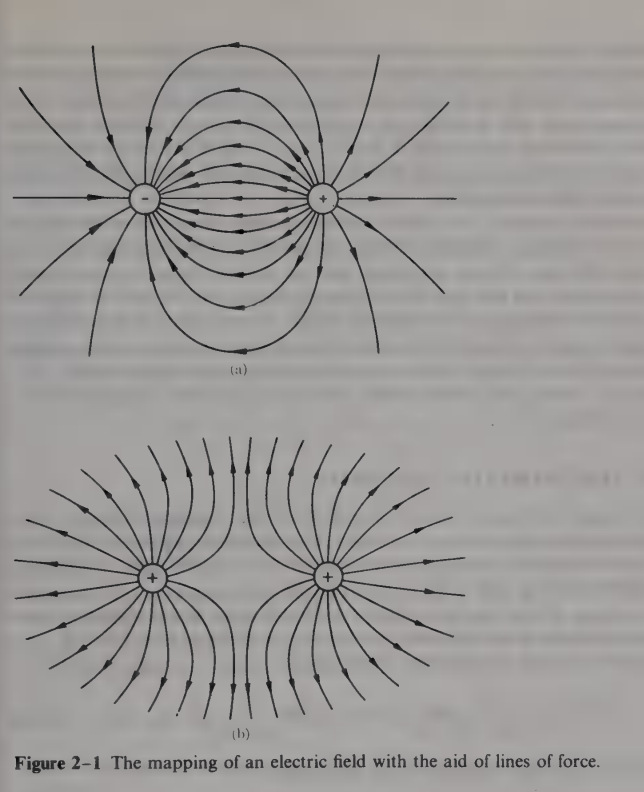
\includegraphics[width=0.3\textwidth]{campo-electric.png}
  \caption{Mapping of an electric field with the aid of lines of force.}
  \label{fig:campo-electric}
\end{figure}

% ========== 2-21 ==========
\begin{enumerate}[label={{\textcolor{trueblue}{\textbf{Pr.} \arabic*.21}}}, start=2]
\item \textbf{Problema 21} \; (a) Show that the force acting on a dipole $\boldsymbol{p}$ placed in an external electric field $\boldsymbol{E}_{\mathrm{ext}}$ is
\[
\boldsymbol{F} \;=\; \boldsymbol{p}\!\cdot\!\boldsymbol{\nabla}\,\boldsymbol{E}_{\mathrm{ext}}.
\]
(b) Show that the torque acting on the dipole in this field is
\[
\boldsymbol{\tau} \;=\; \boldsymbol{r}\times\big[\boldsymbol{p}\!\cdot\!\boldsymbol{\nabla}\,\boldsymbol{E}_{\mathrm{ext}}\big]\;+\; \boldsymbol{p}\times\boldsymbol{E}_{\mathrm{ext}},
\]
where $\boldsymbol{r}$ is the vector distance to the dipole 	from the point about which the torque is to be measured. The quantity $\boldsymbol{p}\times\boldsymbol{E}_{\mathrm{ext}}$, which is independent of the point about which the torque is computed, is called the \emph{turning couple} acting on the dipole.
\end{enumerate}

% ========== 2-22 ==========
\begin{enumerate}[label={{\textcolor{trueblue}{\textbf{Pr.} \arabic*.22}}}, start=2]
\item \textbf{Problema 22} \; Three charges are arranged in a linear array. The charge $-2q$ is placed at the origin, and two charges, each of $+q$, are placed at $(0,0,\ell)$ and $(0,0,-\ell)$, respectively. Find a relatively simple expression for the potential $\varphi(\boldsymbol{r})$ which is valid for distances $\lvert \boldsymbol{r}\rvert \gg \ell$. Make a plot of the equipotential surfaces in the $x,z$–plane.
\end{enumerate}

% ========== 2-23 ==========
\begin{enumerate}[label={{\textcolor{trueblue}{\textbf{Pr.} \arabic*.23}}}, start=2]
\item \textbf{Problema 23} \; What is the quadrupole moment tensor of the charge distribution discussed in Problem 2–22?
\end{enumerate}

% ========== 2-24 ==========
\begin{enumerate}[label={{\textcolor{trueblue}{\textbf{Pr.} \arabic*.24}}}, start=2]
\item \textbf{Problema 24} \; By using delta functions for the charge distribution of point charges, show that the dipole moment of a pair of point charges $\,\boldsymbol{p}=q\,\boldsymbol{\ell}\,$ follows from the general definition
\[
\boldsymbol{p} \;=\; \int \boldsymbol{r}'\,\rho(\boldsymbol{r}')\,d\nu'.
\]
\end{enumerate}

	% ========== 2-25 ==========
\begin{enumerate}[label={{\textcolor{trueblue}{\textbf{Pr.} \arabic*.25}}}, start=2]
\item \textbf{Problema 25} \; Suppose a molecule is represented by a charge $-2q$ at the origin and charges $+q$ at $\boldsymbol{\ell}_1$ and $\boldsymbol{\ell}_2$, with $\lvert \boldsymbol{\ell}_1\rvert=\lvert \boldsymbol{\ell}_2\rvert=\ell$.
\begin{enumerate}[label=(\alph*)]
  \item Find the dipole moment of the molecule.
  \item For $\mathrm{H_2O}$, $\ell=0.958\times 10^{-10}\,\mathrm{m}$ and the angle between $\boldsymbol{\ell}_1$ and $\boldsymbol{\ell}_2$ is $\theta=105^\circ$. If $p=6.14\times 10^{-30}\,\mathrm{C\cdot m}$, find the effective charge $q$.
\end{enumerate}
\end{enumerate}

% ========== 2-26 ==========
\begin{enumerate}[label={{\textcolor{trueblue}{\textbf{Pr.} \arabic*.26}}}, start=2]
\item \textbf{Problema 26} \; Obtain the electric field of a point dipole by calculating the gradient of
\[
\varphi(\boldsymbol{r}) \;=\; \frac{1}{4\pi\epsilon_0}\,\frac{\boldsymbol{p}\cdot\boldsymbol{r}}{r^{3}}.
\]
\end{enumerate}




\section*{\textcolor{Cinnabar}{\textbf{Problemas: cap 3}}}
\addcontentsline{toc}{section}{\textcolor{Cinnabar}{\textbf{Problemas: cap 3}}}

	

% ========== 3-1 ==========
\begin{enumerate}[label={{\textcolor{trueblue}{\textbf{Pr.} \arabic*.1}}}, start=3]
\item \textbf{Problema 1} Two spherical conducting shells of radii $r_{a}$ and $r_{b}$ are arranged concentrically and are charged to the potentials $\varphi_{a}$ and $\varphi_{b}$, respectively . If $r_{b}>r_{a}$, find the potential at points between the shells, and at points $r>r_{b}$
\end{enumerate}

% ========== 3-2 ==========
\begin{enumerate}[label={{\textcolor{trueblue}{\textbf{Pr.} \arabic*.2}}}, start=3]
\item \textbf{Problema 2} Two long cylindrical shells of radii $r_{a}$ and $r_{b}$ are arranged coaxially and are charged to the potentials $\varphi_{a}$ and $\varphi_{b}$, respectively. Find the potential at points between the cylindrical shells.
\end{enumerate}

% ========== 3-3 ==========
\begin{enumerate}[label={{\textcolor{trueblue}{\textbf{Pr.} \arabic*.3}}}, start=3]
\item \textbf{Problema 3} If $\varphi_{1}$ is a solution to Laplace’s equation, prove that the partial derivative of $\varphi_{1}$ with respect to one or more of the rectangular coordinates (e.g., $\partial \varphi_{1}/\partial x$, $\partial^{2}\varphi_{1}/\partial x^{2}$, $\partial^{2}\varphi_{1}/\partial x \partial y$, etc.) is also a solution.
\end{enumerate}

% ========== 3-4 ==========
\begin{enumerate}[label={{\textcolor{trueblue}{\textbf{Pr.} \arabic*.4}}}, start=3]
\item \textbf{Problema 4} Suppose $\varphi$ satisfies Laplace’s equation throughout a region $V_{0}$. Prove that the value of $\varphi$ at any point $O$ is the average of its values over the surface of any sphere centered at $O$ that lies entirely in $V_{0}$:
\[
\varphi(O) = \frac{1}{4\pi R^{2}} \oint \varphi \, da,
\]
where $R$ is the radius of the sphere. \emph{Hint}: Let $\psi = 1/r$ in Eq. (1–57). Show that consequently $\varphi$ has no maxima or minima inside $V_{0}$.
\end{enumerate}

% ========== 3-5 ==========
\begin{enumerate}[label={{\textcolor{trueblue}{\textbf{Pr.} \arabic*.5}}}, start=3]
\item \textbf{Problema 5} Expand the function
\[
F(u) = (1 - 2xu + u^{2})^{-1/2}
\]
in a Taylor series up to the term in $u^{3}$. Note that the coefficients are the first four Legendre polynomials $P_{n}(x)$. In fact, $F(u)$ is a generating function for all the Legendre polynomials:
\[
F(u) = \sum_{n=0}^{\infty} P_{n}(x) u^{n}.
\]
\end{enumerate}
		
% ========== 3-6 ==========
\begin{enumerate}[label={{\textcolor{trueblue}{\textbf{Pr.} \arabic*.6}}}, start=3]
\item \textbf{Problema 6} Show that half the zonal harmonics are generated by differentiating $r^{-1}$ successively with respect to the rectangular coordinate $z$ $(z = r \cos \theta)$.
\end{enumerate}

% ========== 3-7 ==========
\begin{enumerate}[label={{\textcolor{trueblue}{\textbf{Pr.} \arabic*.7}}}, start=3]
\item \textbf{Problema 7} Obtain $\nabla^{2}\varphi$ in cylindrical coordinates, Eq.~(3–8), from the rectangular form, Eq.~(3–6), by direct substitution: $x = r \cos \theta$, $y = r \sin \theta$.

\begin{MyColorPar}{orange(colorwheel)}
\textbf{Eq.~(3–6) Rectangular coordinates:}
\[
\nabla^{2}\varphi = 
\frac{\partial^{2}\varphi}{\partial x^{2}} +
\frac{\partial^{2}\varphi}{\partial y^{2}} +
\frac{\partial^{2}\varphi}{\partial z^{2}} .
\]

\textbf{Eq.~(3–8) Cylindrical coordinates:}
\[
\nabla^{2}\varphi =
\frac{1}{r}\frac{\partial}{\partial r}\!\left(
r \frac{\partial \varphi}{\partial r}\right)
+ \frac{1}{r^{2}}\frac{\partial^{2}\varphi}{\partial \theta^{2}}
+ \frac{\partial^{2}\varphi}{\partial z^{2}} .
\]
\end{MyColorPar}

\end{enumerate}


% ========== 3-8 ==========
\begin{enumerate}[label={{\textcolor{trueblue}{\textbf{Pr.} \arabic*.8}}}, start=3]
\item \textbf{Problema 8} Find the potential of an axial quadrupole: point charges $q$, $-2q$, $q$ placed on the $z$–axis at distances $\ell, 0, -\ell$ from the origin. Find the potential only at distances $r \gg \ell$, and show that this potential is proportional to one of the zonal harmonics.
\end{enumerate}

% ========== 3-9 ==========
\begin{enumerate}[label={{\textcolor{trueblue}{\textbf{Pr.} \arabic*.9}}}, start=3]
\item \textbf{Problema 9} Suppose a point dipole is located at the center of a grounded spherical conducting shell. Find the potential inside the shell. (\emph{Hint}: Use zonal harmonics that are regular at the origin to satisfy the boundary conditions on the shell.)
\end{enumerate}

% ========== 3-10 ==========
\begin{enumerate}[label={{\textcolor{trueblue}{\textbf{Pr.} \arabic*.10}}}, start=3]
\item \textbf{Problema 10} For an uncharged conducting sphere placed in an initially uniform electric field, show that the potential due to the sphere is that of a point dipole and find the induced dipole moment.
\end{enumerate}

% ========== 3-11 ==========
\begin{enumerate}[label={{\textcolor{trueblue}{\textbf{Pr.} \arabic*.11}}}, start=3]
\item \textbf{Problema 11} A conducting sphere of radius $a$ bearing total charge $Q$ is placed in an initially uniform electric field $E_{0}$. Find the potential at all points exterior to the sphere.
\end{enumerate}

% ========== 3-12 ==========
\begin{enumerate}[label={{\textcolor{trueblue}{\textbf{Pr.} \arabic*.12}}}, start=3]
\item \textbf{Problema 12} A long cylindrical conductor of radius $a$ bearing no net charge is placed in an initially uniform electric field $E_{0}$. The direction of $E_{0}$ is perpendicular to the cylinder axis. Find the potential at points exterior to the cylinder, and find also the charge density on the cylindrical surface.
\end{enumerate}

% ========== 3-13 ==========
\begin{enumerate}[label={{\textcolor{trueblue}{\textbf{Pr.} \arabic*.13}}}, start=3]
\item \textbf{Problema 13} Show that $\operatorname{Im}\,A[(x + i y)]^{1/2} = A r^{1/2} \sin \tfrac{1}{2}\theta$ satisfies Laplace’s equation, but that the electric field derived from this function has a discontinuity at $\theta = 0$. (Note that $r$ and $\theta$ are cylindrical coordinates here.) The function may be used to describe the potential at the edge of a charged conducting plane. The conducting plane coincides with the $xz$–plane, but only for positive values of $x$. Find the charge density on the plane. Make a sketch showing several equipotential surfaces and several lines of force.
\end{enumerate}

% ========== 3-14 ==========
\begin{enumerate}[label={{\textcolor{trueblue}{\textbf{Pr.} \arabic*.14}}}, start=3]
\item \textbf{Problema 14} A point charge $q$ is situated a distance $d$ from a grounded conducting plane of infinite extent. Obtain the total charge induced on the plane by direct integration of the surface charge density.
\end{enumerate}

% ========== 3-15 ==========
\begin{enumerate}[label={{\textcolor{trueblue}{\textbf{Pr.} \arabic*.15}}}, start=3]
\item \textbf{Problema 15} Two point charges, $q_{1}$ and $q_{2}$, are located near a grounded conducting plane of infinite extent. Find the image charges which are needed to make the plane a surface of constant potential. From the result just obtained, can you predict the image charge distribution required for the case of a body of arbitrary shape with charge density $\rho$ situated near a conducting plane of infinite extent?
\end{enumerate}

% ========== 3-16 ==========
\begin{enumerate}[label={{\textcolor{trueblue}{\textbf{Pr.} \arabic*.16}}}, start=3]
\item \textbf{Problema 16} Two grounded conducting planes intersect at $60^{\circ}$ and a point charge $q$ lies between them. Determine the positions of the image charges that will give the electric field between the planes.
\end{enumerate}

% ========== 3-17 ==========
\begin{enumerate}[label={{\textcolor{trueblue}{\textbf{Pr.} \arabic*.17}}}, start=3]
\item \textbf{Problema 17} A point charge $q$ is located between two parallel, grounded, conducting planes which are separated by a distance $d$. Find the locations of the infinite number of image charges. Express the force on the charge $q$ by an infinite series.
\end{enumerate}

% ========== 3-18 ==========
\begin{enumerate}[label={{\textcolor{trueblue}{\textbf{Pr.} \arabic*.18}}}, start=3]
\item \textbf{Problema 18} Find the force between a point charge $q$ and an \emph{uncharged} conducting sphere of radius $a$. The point charge is located a distance $r$ from the center of the sphere, where $r > a$. Find an approximate expression valid for $r \gg a$.
\end{enumerate}

% ========== 3-19 ==========
\begin{enumerate}[label={{\textcolor{trueblue}{\textbf{Pr.} \arabic*.19}}}, start=3]
\item \textbf{Problema 19} Show that the problem of an uncharged conducting sphere in an initially uniform electric field $E_{0}$ may be solved by means of images. (\emph{Hint}: A uniform electric field in the vicinity of the origin may be approximated by the field of two point charges $Q$ and $-Q$ placed on the $z$–axis at $z=-L$ and $z=+L$, respectively. The field becomes more nearly uniform as $L \to \infty$. It is evident that
\[
\frac{Q}{2\pi \epsilon_{0} L^{2}} = E_{0}.)
\]
\end{enumerate}

% ========== 3-20 ==========
\begin{enumerate}[label={{\textcolor{trueblue}{\textbf{Pr.} \arabic*.20}}}, start=3]
\item \textbf{Problema 20} A point charge $q$ is located inside and at distance $r$ from the center of a spherical conducting shell. The inner radius of the shell is $a$. Show that this problem can be solved by the image technique, and find the charge density $\sigma$ induced on the inside surface of the shell. (The potential of the spherical shell cannot be completely specified in terms of $q$ and its image, because exterior fixed charges can also contribute. Nevertheless, these exterior charges will add only a constant term to the potential.) Find the total charge induced on the inside surface of the shell (a) by physical arguments, and (b) by integration of $\sigma$ over the surface.
\end{enumerate}

% ========== 3-21 ==========
\begin{enumerate}[label={{\textcolor{trueblue}{\textbf{Pr.} \arabic*.21}}}, start=3]
\item \textbf{Problema 21} A long conducting cylinder bearing a charge $\lambda$ per unit length is oriented parallel to a grounded conducting plane of infinite extent. The axis of the cylinder is at distance $x_{0}$ from the plane, and the radius of the cylinder is $a$. Find the location of the line image, and find also the constant $M$ (which determines the potential of the cylinder) in terms of $a$ and $x_{0}$.
\end{enumerate}

% ========== 3-22 ==========
\begin{enumerate}[label={{\textcolor{trueblue}{\textbf{Pr.} \arabic*.22}}}, start=3]
\item \textbf{Problema 22} A spherical distribution of charge is characterized by a constant charge density $\rho$ for $r \le R$. For radii greater than $R$, the charge density is zero. Find the potential $\varphi(r)$ by integrating Poisson’s equation. Check this result by evaluating the integral (3–1). \emph{Hint}: To perform (3–1), divide the charge region into spherical concentric shells of thickness $dr$.
\end{enumerate}

% ========== 3-23 ==========
\begin{enumerate}[label={{\textcolor{trueblue}{\textbf{Pr.} \arabic*.23}}}, start=3]
\item \textbf{Problema 23} A dipole $\mathbf{p}$ is oriented normal to and at distance $d$ from an infinite conducting plane. The plane is grounded (i.e., at zero potential). Calculate the force exerted on the plane by the dipole.
\end{enumerate}

% ========== 3-24 ==========
\begin{enumerate}[label={{\textcolor{trueblue}{\textbf{Pr.} \arabic*.24}}}, start=3]
\item \textbf{Problema 24} A thunderstorm contains a charge $+Q$ at altitude $h_{1}$ and, directly below this, a charge $-Q$ at altitude $h_{2}$. Find an expression for the vertical electric field $E_{v}$ at the earth’s surface at distance $d$ from the storm. For $h_{1}=5000\,\mathrm{m}$, $h_{2}=3000\,\mathrm{m}$, and $Q=15\,\mathrm{C}$, make a graph showing how $E_{v}$ varies, from $d=0$ to $d=20\,\mathrm{km}$.
\end{enumerate}

% ========== 3-25 ==========
\begin{enumerate}[label={{\textcolor{trueblue}{\textbf{Pr.} \arabic*.25}}}, start=3]
\item \textbf{Problema 25} Suppose $\varphi(x,y,z)$ satisfies Laplace’s equation. Show that the value of $\varphi$ at $(x,y,z)$ is approximately equal to the average of its values at the six surrounding points $(x \pm d, y, z)$, $(x, y \pm d, z)$, $(x, y, z \pm d)$. (\emph{Hint}: Calculate the Taylor series expansion of $\varphi(x + d, y, z)$ up to the term in $d^{3}$, and similarly for the other five points; add the results). Computer programs for the numerical calculation of $\varphi$ can be based on this result.
\end{enumerate}



	





\begin{MyColorPar}{orange(colorwheel)}

\end{MyColorPar}




	
\end{multicols}

\tableofcontents \newpage

\begin{center}
\begin{tikzpicture}
	% Dibuja círculos rellenos en diferentes colores
	\fill[bittersweet] (0,0) circle (0.17cm);
	\fill[Apple Green] (0.6,0) circle (0.17cm);
	\fill[trueblue] (1.2,0) circle (0.17cm);
	\fill[Aguamarina] (1.8,0) circle (0.17cm);
	\fill[Sun] (2.4,0) circle (0.17cm);
	\fill[orange(colorwheel)] (3.0,0) circle (0.17cm);
	\fill[Pesto] (3.6,0) circle (0.17cm);
	\fill[blue-violet] (4.2,0) circle (0.17cm);
	\fill[ticklemepink] (4.8,0) circle (0.17cm);
	\fill[Gallery] (5.4,0) circle (0.17cm);
	\fill[Mantle] (6.0,0) circle (0.17cm);
	\fill[Nevada] (6.6,0) circle (0.17cm);
	\fill[onyx] (7.2,0) circle (0.17cm);
	% Agrega más círculos o modifica los colores según sea necesario
\end{tikzpicture}
\end{center}  \vspace{2cm}

\section{Capítulo 2} \vspace{0.5cm}

\subsection{Problema 1} \vspace{0.5cm}

\textbf{Enunciado.} Dos partículas, cada una de masa $m$ y carga $q$, cuelgan de hilos inextensibles de longitud $l$ sujetos a un mismo punto. Hallar el ángulo $\theta$ que forma cada hilo con la vertical en el equilibrio.

\subsubsection*{Planteamiento físico y geometría}
Por simetría, las cargas se separan horizontalmente el mismo ángulo $\theta$ y quedan a la misma altura. La separación entre ellas es
\begin{equation}\label{eq:distancia}
r \;=\; 2\,l\,\sin\theta.
\end{equation}
Sobre cada partícula actúan: (i) su peso $m\mathbf g$ (vertical hacia abajo), (ii) la tensión $\mathbf T$ del hilo (a lo largo del hilo), y (iii) la fuerza eléctrica de repulsión debida a la otra carga, de módulo
\begin{equation}\label{eq:Fe}
F_e \;=\; \frac{1}{4\pi\varepsilon_0}\,\frac{q^2}{r^2}
\;=\; \frac{k_e q^2}{(2l\sin\theta)^2}
\;=\; \frac{k_e q^2}{4\,l^2\,\sin^2\theta},
\qquad k_e \equiv \frac{1}{4\pi\varepsilon_0}.
\end{equation}

\subsubsection*{Ecuaciones de equilibrio}
Descomponiendo la tensión:
\begin{equation}\label{eq:equilibrio_comp}
\begin{aligned}
\text{(horizontal)}\quad & T\sin\theta \;=\; F_e,\\
\text{(vertical)}\quad & T\cos\theta \;=\; mg.
\end{aligned}
\end{equation}
Dividiendo la primera por la segunda se elimina $T$:
\begin{equation}\label{eq:tan}
\tan\theta \;=\; \frac{F_e}{mg}
\;=\; \frac{k_e q^2}{4\,m g\, l^2}\,\frac{1}{\sin^2\theta}.
\end{equation}
Definimos el parámetro adimensional
\begin{equation}\label{eq:Adef}
A \;\equiv\; \frac{k_e q^2}{4\,m g\, l^2},
\end{equation}
y la condición de equilibrio queda
\begin{equation}\label{eq:cond_equilibrio}
\tan\theta \;=\; \frac{A}{\sin^2\theta}.
\end{equation}

\subsubsection*{Ecuación para $\theta$ y forma implícita de la solución}
Sea $x=\sin\theta\in(0,1)$; usando $\tan\theta=\dfrac{x}{\sqrt{1-x^2}}$ en \eqref{eq:cond_equilibrio}:
\begin{equation}\label{eq:x_equation}
\frac{x}{\sqrt{1-x^2}} \;=\; \frac{A}{x^2}
\;\Longrightarrow\;
x^3 \;=\; A\,\sqrt{1-x^2}.
\end{equation}
Elevando al cuadrado y definiendo $y=x^2=\sin^2\theta$:
\begin{equation}\label{eq:cubica}
y^3 \;+\; A^2\,y \;-\; A^2 \;=\; 0,
\qquad 0<y<1.
\end{equation}
Dado $A$ (fijados $m,\,q,\,l,\,g$), la raíz física $y\in(0,1)$ de \eqref{eq:cubica} determina
\[
\boxed{\;\theta \;=\; \arcsin\!\big(\sqrt{y}\,\big)\;}.
\]
(La \eqref{eq:cubica} puede resolverse numéricamente de forma estable; también admite solución cerrada por Cardano.)

\subsubsection*{Aproximación de ángulo pequeño $\;(\theta\ll 1)$}
Si la repulsión es moderada y $\theta$ es pequeño, $\sin\theta\simeq\theta$ y $\tan\theta\simeq\theta$. Entonces, de \eqref{eq:cond_equilibrio}:
\begin{equation}\label{eq:small_angle}
\theta \;\simeq\; \frac{A}{\theta^2}
\;\Longrightarrow\;
\boxed{\;\theta \;\approx\; \Big(\frac{k_e q^2}{4\,m g\,l^2}\Big)^{\!1/3}\;}.
\end{equation}
Esta expresión es la estimación estándar y resulta muy precisa cuando $\theta$ es de pocos grados.

\subsubsection*{Tensión del hilo (dato útil)}
De \eqref{eq:equilibrio_comp}: $T\cos\theta=mg\ \Rightarrow\ T=\dfrac{mg}{\cos\theta}$, y de forma consistente $T\sin\theta=F_e$ reproduce \eqref{eq:Fe}.

\subsubsection*{Interpretación}
El equilibrio surge del balance entre el peso (que tiende a alinear los hilos verticalmente) y la repulsión eléctrica (que separa las cargas). El parámetro
\[
A=\frac{k_e q^2}{4mgl^2}
\]
mide la \emph{fuerza relativa} de la interacción eléctrica respecto al efecto combinado de la gravedad y la geometría del sistema: a mayor $A$ (cargas más grandes, hilos más cortos o masas más pequeñas), mayor ángulo de apertura $\theta$.

\subsection{Problema 2} \vspace{0.5cm}

\textbf{Enunciado.} Dos esferas conductoras pequeñas e idénticas poseen cargas $2.0\times 10^{-9}\,\mathrm{C}$ y $-0.5\times 10^{-9}\,\mathrm{C}$, respectivamente. Al colocarlas a $4\,\mathrm{cm}$ de separación: (i) hallar la fuerza entre ellas. (ii) Si se ponen en contacto y luego se separan nuevamente $4\,\mathrm{cm}$, hallar la nueva fuerza.

\subsubsection*{Datos}
\[
q_1 = 2.0\times 10^{-9}\,\mathrm{C},\quad
q_2 = -0.5\times 10^{-9}\,\mathrm{C},\quad
r = 4\,\mathrm{cm}=0.040\,\mathrm{m},\quad
k_e=\frac{1}{4\pi\varepsilon_0}\approx 8.9876\times 10^9\,\frac{\mathrm{N\,m^2}}{\mathrm{C^2}}.
\]

\subsubsection*{(i) Fuerza antes del contacto}
Por la ley de Coulomb:
\[
F \;=\; k_e\,\frac{|q_1 q_2|}{r^2}.
\]
Sustituyendo:
\[
F \;=\; (8.9876\times 10^9)\,
\frac{(2.0\times 10^{-9})(0.5\times 10^{-9})}{(0.040)^2}
\;=\; 5.62\times 10^{-6}\,\mathrm{N}.
\]
Como las cargas son de signos opuestos, la fuerza es \textbf{atractiva}. \\
\[
\boxed{\,F_{\text{antes}} \;\approx\; 5.62\times 10^{-6}\ \mathrm{N}\ \text{(atractiva)}\,}.
\]

\subsubsection*{(ii) Contacto, redistribución y nueva fuerza}
Al poner en contacto esferas \emph{idénticas} y conductoras, el potencial común exige que las cargas finales sean iguales. La carga total es
\[
Q_{\text{tot}} = q_1+q_2 = (2.0-0.5)\times 10^{-9} = 1.5\times 10^{-9}\,\mathrm{C}.
\]
Tras el contacto, cada esfera queda con
\[
q' = \frac{Q_{\text{tot}}}{2} = 0.75\times 10^{-9}\,\mathrm{C}.
\]
Separadas otra vez $r=0.040\,\mathrm{m}$, la fuerza (ahora repulsiva, por ser ambas positivas) es
\[
F' \;=\; k_e\,\frac{(q')^2}{r^2}
\;=\; (8.9876\times 10^9)\,
\frac{(0.75\times 10^{-9})^2}{(0.040)^2}
\;=\; 3.16\times 10^{-6}\,\mathrm{N}.
\]
\[
\boxed{\,F_{\text{despu\'es}} \;\approx\; 3.16\times 10^{-6}\ \mathrm{N}\ \text{(repulsiva)}\,}.
\]

\subsubsection*{Comentarios}
\begin{itemize}
  \item La hipótesis de ``esferas pequeñas e idénticas'' permite: (a) despreciar efectos de inducción de forma al evaluar la fuerza como si fuesen puntuales a $r=4\,\mathrm{cm}$; (b) asegurar que, tras el contacto, ambas queden al mismo potencial y, por ser idénticas, con la \emph{misma} carga $q'$.
  \item El cambio de signo (atractiva $\to$ repulsiva) se debe a que, después de compartir carga, ambas quedan con carga positiva.
\end{itemize}



\subsection{Problema 3} \vspace{0.5cm}

\textbf{Enunciado.} Cargas puntuales de $3\times 10^{-9}\,\mathrm{C}$ se colocan en tres vértices de un cuadrado de lado $a=15\,\mathrm{cm}$. Hallar la \textbf{magnitud} y la \textbf{dirección} del campo eléctrico en el vértice vacío.

\subsubsection*{Planteamiento y sistema de coordenadas}
Ubicamos el vértice vacío en el origen $O=(0,0)$ y los otros vértices en
\[
(a,0),\quad (0,a),\quad (a,a),\qquad a=0.15\,\mathrm{m},
\]
cada uno con carga $q=3\times 10^{-9}\,\mathrm{C}$. El campo total en $O$ es la superposición de los campos debidos a las tres cargas.

\subsubsection*{Campo debido a cada carga}
Usamos $k_e=\frac{1}{4\pi\varepsilon_0}$. Definimos la constante
\[
K \;\equiv\; \frac{k_e\,q}{a^2}.
\]
\begin{itemize}
  \item Carga en $(a,0)$: vector posición hacia $O$ es $(-a,0)$, por lo que
  \[
  \mathbf E_{(a,0)} \;=\; -\,K\,\hat{\mathbf x}.
  \]
  \item Carga en $(0,a)$: vector posición hacia $O$ es $(0,-a)$, por lo que
  \[
  \mathbf E_{(0,a)} \;=\; -\,K\,\hat{\mathbf y}.
  \]
  \item Carga en $(a,a)$: distancia $\sqrt{2}\,a$ y dirección hacia $O$ es $(-\hat{\mathbf x}-\hat{\mathbf y})/\sqrt{2}$. Entonces
  \[
  \left\lvert \mathbf E_{(a,a)} \right\rvert \;=\; \frac{k_e q}{(\sqrt{2}\,a)^2} \;=\; \frac{K}{2},
  \qquad
  \mathbf E_{(a,a)} \;=\; \frac{K}{2}\,\frac{-\hat{\mathbf x}-\hat{\mathbf y}}{\sqrt{2}}
  \;=\; -\,\frac{K}{2\sqrt{2}}\hat{\mathbf x}\;-\;\frac{K}{2\sqrt{2}}\hat{\mathbf y}.
  \]
\end{itemize}

\subsubsection*{Suma vectorial}
\[
\mathbf E(O) \;=\; \mathbf E_{(a,0)}+\mathbf E_{(0,a)}+\mathbf E_{(a,a)}
\;=\; \bigg[-K-\frac{K}{2\sqrt{2}}\bigg]\hat{\mathbf x}
\;+\; \bigg[-K-\frac{K}{2\sqrt{2}}\bigg]\hat{\mathbf y}.
\]
Es decir,
\[
E_x=E_y \;=\; -\,K\Big(1+\frac{1}{2\sqrt{2}}\Big).
\]

\subsubsection*{Magnitud y dirección}
Como $E_x=E_y$ (ambos negativos), el vector apunta a lo largo de $-\hat{\mathbf x}-\hat{\mathbf y}$, es decir, \textbf{sobre la diagonal hacia el interior del cuadrado}, formando $45^\circ$ con el eje $-x$ (ángulo $225^\circ$ desde $+x$).

La magnitud es
\[
\lvert \mathbf E \rvert
=\sqrt{E_x^2+E_y^2}
=\sqrt{2}\,K\Big(1+\frac{1}{2\sqrt{2}}\Big)
= K\Big(\sqrt{2}+\frac{1}{2}\Big).
\]

\subsubsection*{Valor numérico}
Con $k_e\simeq 8.9876\times 10^9\,\mathrm{N\,m^2/C^2}$, $q=3\times 10^{-9}\,\mathrm{C}$ y $a=0.15\,\mathrm{m}$:
\[
K=\frac{k_e q}{a^2}=
\frac{(8.9876\times 10^9)(3\times 10^{-9})}{(0.15)^2}
\;\approx\; 1.198\times 10^{3}\ \mathrm{V/m}.
\]
Por tanto,
\[
\boxed{\;
\lvert \mathbf E \rvert \;\approx\; K\!\left(\sqrt{2}+\tfrac{1}{2}\right)
\;\approx\; 2.29\times 10^{3}\ \mathrm{V/m},
\quad
\text{dirección: a lo largo de } \frac{-\hat{\mathbf x}-\hat{\mathbf y}}{\sqrt{2}}\;(225^\circ).\;
}
\]


\subsection{Problema 4} \vspace{0.5cm}

\textbf{Enunciado.} Una línea de carga infinitamente larga tiene densidad uniforme $\lambda$ (carga por unidad de longitud). Usando \emph{integración directa}, encontrar el campo eléctrico a una distancia $r$ de la línea.

\subsubsection*{Planteamiento y simetría}
Coloquemos la línea de carga a lo largo del eje $z$ y el punto de observación en el plano $xy$ a distancia $r$ del eje (por ejemplo, en $(r,0,0)$). Por simetría cilíndrica:
\begin{itemize}
  \item El campo $\mathbf{E}$ es estrictamente \textbf{radial} (dirección $\hat{\mathbf r}$).
  \item Su magnitud sólo depende de la distancia $r$.
  \item Las componentes a lo largo de $z$ se cancelan por simetría al integrar de $-\infty$ a $+\infty$.
\end{itemize}

\subsubsection*{Integración directa}
Tomemos un elemento de carga $dq=\lambda\,dz'$ situado en $z'$ sobre el eje $z$. La distancia al punto de observación es
\[
s \;=\; \sqrt{r^2 + z'^2}.
\]
El campo diferencial (Ley de Coulomb) es
\[
dE \;=\; \frac{1}{4\pi\varepsilon_0}\,\frac{dq}{s^2}
\;=\; \frac{1}{4\pi\varepsilon_0}\,\frac{\lambda\,dz'}{r^2+z'^2}.
\]
Su componente radial es $dE_r = dE\,\cos\alpha$, con $\cos\alpha = \dfrac{r}{s}$:
\[
dE_r \;=\; \frac{1}{4\pi\varepsilon_0}\,\frac{\lambda\,dz'}{r^2+z'^2}\,\frac{r}{\sqrt{r^2+z'^2}}
\;=\; \frac{\lambda r}{4\pi\varepsilon_0}\,\frac{dz'}{(r^2+z'^2)^{3/2}}.
\]
Integrando de $z'=-\infty$ a $+\infty$:
\[
E_r(r) \;=\; \frac{\lambda r}{4\pi\varepsilon_0}\,\int_{-\infty}^{+\infty}\frac{dz'}{(r^2+z'^2)^{3/2}}.
\]
La primitiva útil es
\[
\int \frac{dz'}{(r^2+z'^2)^{3/2}} \;=\; \frac{z'}{r^2\sqrt{r^2+z'^2}} \;+\; C,
\]
de modo que
\[
\int_{-\infty}^{+\infty}\frac{dz'}{(r^2+z'^2)^{3/2}}
\;=\;
\left.\frac{z'}{r^2\sqrt{r^2+z'^2}}\right|_{-\infty}^{+\infty}
\;=\; \frac{1}{r^2} - \left(-\frac{1}{r^2}\right)
\;=\; \frac{2}{r^2}.
\]
Sustituyendo:
\[
E_r(r) \;=\; \frac{\lambda r}{4\pi\varepsilon_0}\,\frac{2}{r^2}
\;=\; \boxed{\,\frac{\lambda}{2\pi\varepsilon_0\,r}\,}.
\]

\subsubsection*{Dirección y comentario}
\[
\boxed{\;\mathbf{E}(r)\;=\;\frac{\lambda}{2\pi\varepsilon_0\,r}\,\hat{\mathbf r}\;}
\quad\text{(apunta radialmente hacia afuera si $\lambda>0$, hacia adentro si $\lambda<0$).}
\]
Este resultado coincide con el que se obtiene por la Ley de Gauss usando una superficie cilíndrica coaxial de radio $r$ y altura $L$.

\subsection{Problema 5} \vspace{0.5cm}

\textbf{Enunciado.} 
(a) Un disco circular de radio $R$ tiene densidad superficial uniforme de carga $\sigma$.\footnote{En la redacción original aparece $\rho$; aquí usamos la notación estándar $\sigma$ para \emph{densidad superficial}.} Hallar el campo eléctrico en un punto del eje del disco a una distancia $z$ del plano del disco. 

(b) Un cilindro circular recto de radio $R$ y altura $L$ está orientado a lo largo del eje $z$ (centro en el origen). Tiene densidad de carga volumétrica no uniforme
\[
\rho(z)=\rho_0+\beta z.
\]
Hallar la \textbf{fuerza} sobre una carga puntual $q$ situada en el \emph{centro} del cilindro.

% ===========================================================
\subsubsection*{(a) Campo en el eje de un disco uniformemente cargado}

\paragraph{1) Método de integración por anillos (derivación completa).}
Por simetría, el campo en el punto $P=(0,0,z)$ es axial: $\mathbf E(P)=E_z(z)\,\hat{\mathbf z}$.  
Dividimos el disco en anillos concéntricos de radio $r'$ y espesor $dr'$, cada uno con carga $dq=\sigma\,2\pi r'\,dr'$.

Distancia del anillo a $P$:
\[
s=\sqrt{r'^2+z^2},\qquad \cos\alpha=\frac{z}{s}.
\]
Con la ley de Coulomb, la contribución axial es
\[
dE_z=\frac{1}{4\pi\varepsilon_0}\frac{dq}{s^2}\cos\alpha
= \frac{1}{4\pi\varepsilon_0}\frac{\sigma\,2\pi r'\,dr'}{r'^2+z^2}\,\frac{z}{\sqrt{r'^2+z^2}}
= \frac{\sigma z}{2\varepsilon_0}\,\frac{r'\,dr'}{(r'^2+z^2)^{3/2}}.
\]
Integramos $r'\in[0,R]$:
\[
E_z(z)=\frac{\sigma z}{2\varepsilon_0}\int_0^{R}\frac{r'\,dr'}{(r'^2+z^2)^{3/2}}
= \frac{\sigma z}{2\varepsilon_0}\left[-\frac{1}{\sqrt{r'^2+z^2}}\right]_{0}^{R}.
\]
Por tanto,
\begin{equation}\label{eq:Ez-disco}
\boxed{\,E_z(z)=\frac{\sigma}{2\varepsilon_0}\left(1-\frac{z}{\sqrt{z^2+R^2}}\right),\qquad \mathbf E=E_z\,\hat{\mathbf z}. \,}
\end{equation}

\paragraph{2) Potencial primero, campo después (alternativa útil).}
El potencial sobre el eje (referido a $V(\infty)=0$) se obtiene sumando contribuciones de anillos:
\[
dV=\frac{1}{4\pi\varepsilon_0}\frac{dq}{s}
=\frac{1}{4\pi\varepsilon_0}\frac{\sigma\,2\pi r'\,dr'}{\sqrt{r'^2+z^2}}
\ \Rightarrow\
V(z)=\frac{\sigma}{2\varepsilon_0}\!\int_0^R\!\frac{r'\,dr'}{\sqrt{r'^2+z^2}}
=\frac{\sigma}{2\varepsilon_0}\big(\sqrt{z^2+R^2}-|z|\big).
\]
Luego $E_z=-\,dV/dz$ reproduce \eqref{eq:Ez-disco}.  

\paragraph{3) Chequeos de consistencia y límites.}
\[
\begin{aligned}
&\text{Plano infinito: } \lim_{z\to 0^+}E_z=\frac{\sigma}{2\varepsilon_0}.\\
&\text{Campo lejano: } z\gg R\ \Rightarrow\ \sqrt{z^2+R^2}\simeq z+\frac{R^2}{2z},\
E_z\simeq \frac{\sigma}{2\varepsilon_0}\frac{R^2}{2z^2}
=\frac{1}{4\pi\varepsilon_0}\frac{Q}{z^2},\ \ Q=\sigma\pi R^2.\\
&\text{Continuidad de }E_z:\ \text{el salto en la superficie es } \Delta E_n=\sigma/\varepsilon_0\ \text{(dos caras).}
\end{aligned}
\]

\paragraph{4) Señales y dirección.}
Si $\sigma>0$, entonces $E_z(z)>0$ para $z>0$ (sale del disco) y $E_z(z)<0$ para $z<0$ (entra al disco).

\paragraph{5) Expansiones útiles (para bosquejos rápidos).}
\[
\begin{aligned}
&z\ll R:\quad E_z(z)\approx \frac{\sigma}{2\varepsilon_0}\left(1-\frac{z}{R}+\frac{z^3}{2R^3}+\cdots\right).\\
&z\gg R:\quad E_z(z)\approx \frac{1}{4\pi\varepsilon_0}\frac{Q}{z^2}\left(1-\frac{3R^2}{8z^2}+\cdots\right).
\end{aligned}
\]

\bigskip
% ===========================================================
\subsubsection*{(b) Fuerza sobre $q$ en el centro de un cilindro con $\rho(z)=\rho_0+\beta z$}

\paragraph{1) Simetría y reducción.}
En el centro $O$ sólo puede haber componente axial: $\mathbf E(O)=E_z(0)\,\hat{\mathbf z}$.  
Las componentes radiales se anulan por simetría al integrar en $\phi$. La densidad $\rho_0$ es \emph{par} en $z$ y no contribuye al campo en $O$ (cancelación arriba/abajo). La parte \emph{impar} $\beta z$ sí contribuye.

\paragraph{2) Integración directa del campo en $O$.}
Elemento de volumen en cilíndricas: $dV=r'\,dr'\,d\phi'\,dz$, con $r'\in[0,R]$, $z\in[-L/2,L/2]$.  
La contribución axial de $dQ=\rho(z)\,dV$ es
\[
dE_z=-\frac{1}{4\pi\varepsilon_0}\frac{\rho(z)\,z}{(r'^2+z^2)^{3/2}}\,r'\,dr'\,d\phi'\,dz.
\]
Integramos en $\phi'$ (factor $2\pi$) y en $r'$:
\[
E_z(0)=-\frac{1}{2\varepsilon_0}\int_{-L/2}^{L/2}\rho(z)\,\Bigg[\int_0^R\frac{r'\,dr'}{(r'^2+z^2)^{3/2}}\Bigg]dz.
\]
La integral radial es estándar:
\[
\int_0^R\frac{r'\,dr'}{(r'^2+z^2)^{3/2}}
=\left[\frac{1}{|z|}-\frac{1}{\sqrt{R^2+z^2}}\right].
\]
Sustituyendo y separando $\rho(z)=\rho_0+\beta z$:
\[
E_z(0)=-\frac{1}{2\varepsilon_0}\int_{-L/2}^{L/2}\!\left\{\rho_0\!\left[\frac{1}{|z|}-\frac{1}{\sqrt{R^2+z^2}}\right]+\beta z\!\left[\frac{1}{|z|}-\frac{1}{\sqrt{R^2+z^2}}\right]\right\}\!dz.
\]
\textbf{Cancelación de la parte par $\rho_0$:} el integrando con $\rho_0$ es \emph{impar} en torno a $z=0$ (por el $1/|z|$ se ve descompuesto como $\operatorname{sgn}(z)$ al multiplicar por $z$ al derivar; riguroso: integrar en $z>0$ y $z<0$ y sumar) $\Rightarrow$ contribución nula.  
Queda sólo el término con $\beta z$:
\[
E_z(0)=-\frac{\beta}{2\varepsilon_0}\int_{-L/2}^{L/2}\!\left[\,|z|-\frac{z^2}{\sqrt{R^2+z^2}}\,\right]dz
= -\frac{\beta}{\varepsilon_0}\left[\int_{0}^{L/2}\! z\,dz-\int_{0}^{L/2}\!\frac{z^2}{\sqrt{R^2+z^2}}\,dz\right].
\]
La primera integral es $L^2/8$. Para la segunda usamos $z=R\sinh t$:
\[
\int_{0}^{L/2}\!\frac{z^2}{\sqrt{R^2+z^2}}\,dz
= R^2\!\int_{0}^{\operatorname{arsinh}\!\left(\frac{L}{2R}\right)}\!\sinh^2 t\,dt
= \frac{R L}{4}\sqrt{1+\Big(\tfrac{L}{2R}\Big)^2}-\frac{R^2}{2}\operatorname{arsinh}\!\Big(\tfrac{L}{2R}\Big).
\]
Con esto obtenemos la forma \emph{exacta}:
\begin{equation}\label{eq:Ez-cilindro-exacta}
\boxed{\
E_z(0)\;=\;-\frac{\beta}{\varepsilon_0}\left[
\frac{L^2}{8}
- \frac{R L}{4}\sqrt{1+\Big(\frac{L}{2R}\Big)^2}
+ \frac{R^2}{2}\operatorname{arsinh}\!\Big(\frac{L}{2R}\Big)
\right],\qquad \mathbf E(0)=E_z(0)\,\hat{\mathbf z}.
}
\end{equation}
Finalmente, la \textbf{fuerza} sobre la carga $q$ en el centro:
\begin{equation}\label{eq:F-cilindro}
\boxed{\ \mathbf F\;=\;q\,\mathbf E(0)\;=\; -\,\frac{q\,\beta}{\varepsilon_0}\left[
\frac{L^2}{8}
- \frac{R L}{4}\sqrt{1+\Big(\frac{L}{2R}\Big)^2}
+ \frac{R^2}{2}\operatorname{arsinh}\!\Big(\frac{L}{2R}\Big)
\right]\hat{\mathbf z}\ .}
\end{equation}

\paragraph{3) Análisis físico y de signos.}
\begin{itemize}
\item Si $\beta>0$ (la densidad crece con $z$), hay \emph{más} carga en la mitad superior; el corchete en \eqref{eq:Ez-cilindro-exacta} es positivo $\Rightarrow E_z(0)<0$: el campo apunta hacia abajo (hacia la región de menor carga). Para $q>0$, la fuerza también apunta hacia $-\,\hat{\mathbf z}$.
\item La parte constante $\rho_0$ no contribuye al campo en el centro (simetría par en $z$).
\end{itemize}

\paragraph{4) Forma adimensional y límites útiles.}
Sea $u\equiv L/(2R)$. Entonces
\[
E_z(0)=-\frac{\beta R^2}{\varepsilon_0}\left[u^2-\;u\sqrt{1+u^2}\;+\;\operatorname{arsinh}u\right].
\]
\textbf{Cilindro muy largo} ($u\gg 1$):
\[
\sqrt{1+u^2}\sim u+\frac{1}{2u},\quad \operatorname{arsinh}u\sim \ln(2u)+\frac{1}{4u^2},
\]
\[
E_z(0)\ \simeq\ -\frac{\beta}{\varepsilon_0}\left[\frac{R^2}{2}\ln\!\Big(\frac{L}{R}\Big)\;+\;\frac{R^2}{4}\right]\quad(\text{crece lentamente con }\ln(L/R)).
\]
\textbf{Cilindro “chato”} ($u\ll 1$):
\[
E_z(0)\approx -\frac{\beta}{\varepsilon_0}\,\frac{L^4}{192\,R^2}\;\;\to 0
\qquad (\text{casi simetría arriba/abajo}).
\]

\paragraph{5) Verificación dimensional.}
En \eqref{eq:F-cilindro}, $[\beta]=\mathrm{C\,m^{-4}}$ (pues $\rho=\rho_0+\beta z$) y el factor entre corchetes tiene dimensión $m^2$, por lo que $E\sim (\beta m^2)/\varepsilon_0$ (V/m), y $F=qE$ (N): consistente.

\paragraph{6) Comentario alternativo (momento dipolar del volumen).}
La parte impar $\rho(z)=\beta z$ genera un \emph{momento dipolar} neto $\mathbf p=\hat{\mathbf z}\int z\,\rho(z)\,dV$ distinto de cero. Aunque el campo de un dipolo puro se evalúa típicamente \emph{lejos} del volumen, esta observación explica que el campo en el centro no se anule cuando hay una ligera asimetría lineal en $z$.

% ===========================================================
\paragraph{Resumen del Problema 5.}
\begin{itemize}
\item \textbf{Disco uniforme sobre el eje:} $\displaystyle E_z(z)=\frac{\sigma}{2\varepsilon_0}\left(1-\frac{z}{\sqrt{z^2+R^2}}\right)$, \ 
$V(z)=\dfrac{\sigma}{2\varepsilon_0}\left(\sqrt{z^2+R^2}-|z|\right)$.
\item \textbf{Cilindro con $\rho(z)=\rho_0+\beta z$ (en el centro):} Sólo contribuye la parte $\beta z$.  
Campo exacto en \eqref{eq:Ez-cilindro-exacta} y fuerza en \eqref{eq:F-cilindro}.
\end{itemize}

\subsection{Problema 6} \vspace{0.5cm}

\textbf{Enunciado.} Una cáscara esférica conductora delgada, de radio $R$, está cargada \emph{uniformemente} con carga total $Q$. Por \emph{integración directa}, hallar el potencial en un punto arbitrario (a) \emph{dentro} de la cáscara, (b) \emph{fuera} de la cáscara.

\subsubsection*{Datos y simetría}
La densidad superficial es
\[
\sigma=\frac{Q}{4\pi R^2}.
\]
Por simetría esférica, el potencial depende sólo de $r=|\mathbf r|$. Partimos de la definición integral
\[
V(\mathbf r)=\frac{1}{4\pi\varepsilon_0}\int_{S}\frac{\sigma\,dA'}{|\mathbf r-\mathbf r'|},
\qquad |\mathbf r'|=R.
\]
Elegimos el eje polar a lo largo de $\mathbf r$; así el integrando depende sólo del ángulo polar $\theta'$ entre $\mathbf r$ y $\mathbf r'$.

\subsubsection*{Geometría del integrando y reducción angular}
Con esa elección,
\[
|\mathbf r-\mathbf r'|=\sqrt{r^2+R^2-2rR\cos\theta'}\equiv s(\theta'),\qquad
dA'=R^2\sin\theta'\,d\theta'\,d\phi'.
\]
La integral en $\phi'$ da $2\pi$, y usando $\mu=\cos\theta'$ ($d\mu=-\sin\theta'\,d\theta'$) queda
\[
V(r)=\frac{\sigma}{4\pi\varepsilon_0}\,(2\pi R^2)\int_{-1}^{1}\frac{d\mu}{\sqrt{r^2+R^2-2rR\mu}}.
\]
La primitiva elemental
\[
\int\frac{d\mu}{\sqrt{a-b\mu}}=-\frac{2}{b}\sqrt{a-b\mu}+C,\qquad a=r^2+R^2,\;\;b=2rR,
\]
da
\[
\int_{-1}^{1}\frac{d\mu}{\sqrt{r^2+R^2-2rR\mu}}
=\frac{1}{rR}\,\Big[(r+R)-|r-R|\Big].
\]

\subsubsection*{(a) Potencial \texorpdfstring{$r<R$}{r<R} (interior)}
Si $r<R$, entonces $|r-R|=R-r$, y
\[
\int_{-1}^{1}\cdots=\frac{1}{rR}\big[(r+R)-(R-r)\big]=\frac{2}{R}.
\]
Luego
\[
V(r)=\frac{\sigma}{4\pi\varepsilon_0}(2\pi R^2)\frac{2}{R}
=\frac{\sigma}{4\pi\varepsilon_0}(4\pi R)
=\boxed{\,\frac{Q}{4\pi\varepsilon_0\,R}\,},\qquad (r<R).
\]
\emph{Conclusión:} $V$ es \textbf{constante} en todo el interior (como requiere un conductor en equilibrio).

\subsubsection*{(b) Potencial \texorpdfstring{$r>R$}{r>R} (exterior)}
Si $r>R$, entonces $|r-R|=r-R$, y
\[
\int_{-1}^{1}\cdots=\frac{1}{rR}\big[(r+R)-(r-R)\big]=\frac{2}{r}.
\]
Así,
\[
V(r)=\frac{\sigma}{4\pi\varepsilon_0}(2\pi R^2)\frac{2}{r}
=\frac{\sigma}{4\pi\varepsilon_0}\frac{4\pi R^2}{r}
=\boxed{\,\frac{Q}{4\pi\varepsilon_0\,r}\,},\qquad (r>R).
\]
\emph{Conclusión:} exteriormente la cáscara equivale a una \textbf{carga puntual} $Q$ en el centro.

\subsubsection*{Campo eléctrico y condiciones en la superficie}
Derivando $V$:
\[
\mathbf E(r)=-\nabla V=
\begin{cases}
\mathbf 0, & r<R,\\[4pt]
\dfrac{Q}{4\pi\varepsilon_0 r^2}\,\hat{\mathbf r}, & r>R.
\end{cases}
\]
$V$ es \textbf{continuo} en $r=R$: $V(R^-)=V(R^+)=Q/(4\pi\varepsilon_0R)$.  
El campo normal presenta el salto
\[
E_n(R^+)-E_n(R^-)=\frac{\sigma}{\varepsilon_0},
\]
en acuerdo con las condiciones de frontera en conductores.

\subsubsection*{Chequeo alternativo (ley de Gauss)}
Una superficie gaussiana esférica de radio $r$ encierra:
\[
Q_{\rm enc}=
\begin{cases}
0, & r<R,\\
Q, & r>R.
\end{cases}
\quad\Rightarrow\quad
\oint \mathbf E\cdot d\mathbf a=\dfrac{Q_{\rm enc}}{\varepsilon_0}
\ \Rightarrow\
E(r)=
\begin{cases}
0, & r<R,\\
\dfrac{Q}{4\pi\varepsilon_0 r^2}, & r>R,
\end{cases}
\]
lo que es consistente con los resultados obtenidos por integración directa del potencial.

\subsubsection*{Notas y extensiones útiles}
\begin{itemize}
\item Si la cáscara tuviera radio $R$ pero no fuese conductora y la carga no fuese estrictamente superficial, $V(r)$ interior no sería constante. El carácter conductor (carga en la superficie y $E=0$ en el metal) es clave.
\item Para varias cáscaras concéntricas, $V$ se obtiene por superposición; en regiones intermedias $V(r)$ es del tipo $A+B/r$ y se determinan $A,B$ por continuidad de $V$ y salto de $E_n$.
\end{itemize}


\subsection{Problema 7} \vspace{0.5cm}

\textbf{Enunciado.} Dos cargas puntuales
\[
-q \quad \text{(en el origen)} \qquad \text{y} \qquad \pm \frac{q}{2} \quad \text{(en } (a,0,0)\text{)}
\]
están situadas sobre el eje $x$. (i) ¿En qué punto del eje $x$ se anula el campo eléctrico? (ii) En el plano $x$–$y$, haga una gráfica de la \emph{equipotencial} que pasa por dicho punto. (iii) ¿Es ese punto un mínimo verdadero del potencial?

\subsubsection*{Planteamiento general}
Sobre el eje $x$ el campo es colineal con $\hat{\mathbf x}$. Para una carga $q_i$ en $x_i$,
\[
E_x(x)=\frac{1}{4\pi\varepsilon_0}\sum_i q_i\,\frac{\operatorname{sgn}(x-x_i)}{(x-x_i)^2},
\]
ya que el campo de una carga positiva apunta \emph{hacia afuera} (signo de $x-x_i$), y el de una carga negativa, \emph{hacia ella} (cambia el signo por $q_i<0$).

Nuestro sistema:
\[
q_1=-q \ \text{en}\ x_1=0,\qquad q_2=\pm \frac{q}{2}\ \text{en}\ x_2=a.
\]
Entonces
\[
E_x(x)=\frac{k q}{1}\left[\,\frac{-\,\operatorname{sgn}(x)}{x^2}\;+\;\frac{\pm \tfrac12\,\operatorname{sgn}(x-a)}{(x-a)^2}\,\right],
\qquad k\equiv \frac{1}{4\pi\varepsilon_0}.
\]
Buscamos $E_x(x)=0$ por regiones.

\subsubsection*{Caso A: $q_2=+\dfrac{q}{2}$ (cargas de signo \emph{opuesto})}
\paragraph{Región I: $x<0$.} $\operatorname{sgn}(x)= -1$, $\operatorname{sgn}(x-a)=-1$.
\[
E_x=kq\left[\,\frac{-(-1)}{x^2}+\frac{(+\tfrac12)(-1)}{(x-a)^2}\right]
= kq\left(\frac{1}{x^2}-\frac{1}{2(x-a)^2}\right).
\]
Anular $E_x$:
\[
\frac{1}{x^2}=\frac{1}{2(x-a)^2}
\;\Longrightarrow\;
(x-a)^2=2x^2
\;\Longrightarrow\;
x-a=\sqrt{2}\,x\quad(\text{aquí }x<0\Rightarrow\text{signo consistente}),
\]
\[
\boxed{\,x=\frac{a}{1-\sqrt{2}}=-(\sqrt{2}+1)\,a\,}\quad(\text{a la izquierda de ambas cargas}).
\]

\paragraph{Región II: $0<x<a$.} $\operatorname{sgn}(x)=+1$, $\operatorname{sgn}(x-a)=-1$.
\[
E_x=kq\left[-\frac{1}{x^2}-\frac{1}{2(x-a)^2}\right]<0\quad\Rightarrow\ \text{no hay solución}.
\]

\paragraph{Región III: $x>a$.} $\operatorname{sgn}(x)=+1$, $\operatorname{sgn}(x-a)=+1$.
\[
E_x=kq\left[-\frac{1}{x^2}+\frac{1}{2(x-a)^2}\right]=0
\ \Longrightarrow\
x^2=2(x-a)^2.
\]
Tomando $x> a$:
\[
x=\sqrt{2}(x-a)\ \Rightarrow\ (\sqrt{2}-1)x=\sqrt{2}\,a
\ \Rightarrow\
\boxed{\,x=(2+\sqrt{2})\,a\,}.
\]

\emph{Conclusión (Caso A):} el campo se anula en \textbf{dos} puntos del eje,
\[
x_1=-(\sqrt{2}+1)a,\qquad x_2=(2+\sqrt{2})a,
\]
y \emph{no} entre las cargas (como es típico en cargas de signos opuestos: allí los campos se suman, no se cancelan).

\subsubsection*{Caso B: $q_2=-\dfrac{q}{2}$ (cargas de \emph{igual} signo, ambas negativas)}
\paragraph{Región II: $0<x<a$.} $\operatorname{sgn}(x)=+1$, $\operatorname{sgn}(x-a)=-1$.
\[
E_x=kq\left[-\frac{1}{x^2}+\frac{(+)(-\,\tfrac12)}{(x-a)^2}\right]
= kq\left[-\frac{1}{x^2}+\frac{1}{2(a-x)^2}\right].
\]
Imponiendo $E_x=0$:
\[
\frac{1}{x^2}=\frac{1}{2(a-x)^2}\ \Rightarrow\ x^2=2(a-x)^2
\ \Rightarrow\ x=\sqrt{2}(a-x)\ (0<x<a),
\]
\[
x(1+\sqrt{2})=\sqrt{2}\,a\ \Rightarrow\ 
\boxed{\,x=\frac{\sqrt{2}}{1+\sqrt{2}}\,a=(2-\sqrt{2})\,a\approx 0.586\,a\,}.
\]
\paragraph{Regiones $x<0$ y $x>a$.} El campo no puede anularse (los aportes tienen \emph{el mismo} signo y se suman).\\[2pt]
\emph{Conclusión (Caso B):} hay un único punto de anulación entre las dos cargas, en $x=(2-\sqrt{2})a$.

\subsubsection*{Equipotencial que pasa por el punto hallado}
El potencial en el plano $x$–$y$ (con $z=0$) es
\[
V(x,y)=k\left[\frac{-q}{\sqrt{x^2+y^2}}+\frac{\pm \tfrac{q}{2}}{\sqrt{(x-a)^2+y^2}}\right].
\]
Sea $x_\star$ cualquiera de los puntos donde $E_x=0$ (según el caso). La \emph{equipotencial} buscada es el \emph{lugar} de puntos $(x,y)$ que satisfacen
\[
V(x,y)=V(x_\star,0)
= k\left[\frac{-q}{|x_\star|}+\frac{\pm \tfrac{q}{2}}{|x_\star-a|}\right].
\]
En la práctica, para bosquejarla:
\begin{itemize}
\item Traza los focos en $(0,0)$ y $(a,0)$.
\item Dibuja la curva de nivel de $V$ que pasa por $(x_\star,0)$: es cerrada alrededor de la carga \emph{dominante} del signo de $V(x_\star,0)$ y se deforma por la otra; en cortes $y=\text{cte}$ se obtiene resolviendo una ecuación en $x$ con dos distancias radiales.
\end{itemize}
(\emph{Nota:} a diferencia de $V=0$ para dos cargas de signos opuestos —que da un lugar \emph{circular} tipo Apolonio— aquí el nivel $V=V(x_\star,0)$ no es, en general, una circunferencia exacta).

\subsubsection*{¿Es un mínimo verdadero de $V$?}
No. En cualquier región sin carga, $V$ satisface \textbf{Laplace} ($\nabla^2 V=0$), que prohíbe máximos o mínimos locales verdaderos del potencial (principio del máximo). Por tanto, un punto donde $\nabla V=\mathbf 0$ en el vacío sólo puede ser un \textbf{punto silla} (saddle).\\[2pt]
\emph{Conclusión:} el punto donde $E=\mathbf 0$ no es un mínimo verdadero de $V$; es un punto silla (estable en una dirección y inestable en otra).

\subsubsection*{Resumen}
\[
\boxed{\text{Caso }(+):\ E=0\ \text{en}\ x=-(\sqrt{2}+1)a\ \text{y}\ x=(2+\sqrt{2})a\ \ (\text{no entre cargas}).}
\]
\[
\boxed{\text{Caso }(-):\ E=0\ \text{único en}\ x=(2-\sqrt{2})a\in(0,a).}
\]
La equipotencial que pasa por ese punto es la curva $V(x,y)=V(x_\star,0)$; y el punto es \textbf{punto silla}, no mínimo.


\subsection{Problema 8} \vspace{0.5cm}

\textbf{Enunciado.} Muestre que la equipotencial $U=0$ del problema anterior es \emph{esférica}. ¿Cuáles son las coordenadas del centro de esa esfera?

\subsubsection*{Contexto (desde el Pr.~7)}
Tenemos dos cargas sobre el eje $x$:
\[
q_1=-q \ \text{en}\ (0,0,0), \qquad q_2=+\frac{q}{2}\ \text{en}\ (a,0,0).
\]
(Si $q_2=-\tfrac{q}{2}$ entonces $V<0$ en todo el espacio y \emph{no} existe superficie $V=0$.)

El potencial en un punto $\mathbf r=(x,y,z)$ es
\[
V(\mathbf r)=\frac{1}{4\pi\varepsilon_0}\left(\frac{-q}{r_1}+\frac{+\frac{q}{2}}{r_2}\right),
\qquad
r_1=\sqrt{x^2+y^2+z^2},\quad
r_2=\sqrt{(x-a)^2+y^2+z^2}.
\]
La condición $V=0$ (equipotencial buscada) se reduce a
\[
\frac{-q}{r_1}+\frac{+\frac{q}{2}}{r_2}=0
\quad\Longleftrightarrow\quad
\boxed{\,r_2=\frac{1}{2}\,r_1\,}.
\]
Este es un \emph{lugar de Apolonio}: el conjunto de puntos cuya distancia a dos focos cumple una razón constante $k=\tfrac{1}{2}\neq 1$. En $\mathbb{R}^3$ ese lugar es una \textbf{esfera}.

\subsubsection*{Derivación explícita (forma cartesiana)}
Partimos de $r_2=\tfrac{1}{2}r_1$ y elevamos al cuadrado:
\[
(x-a)^2+y^2+z^2=\frac{1}{4}\,(x^2+y^2+z^2).
\]
Llevando términos a un lado:
\[
\left(1-\frac{1}{4}\right)(x^2+y^2+z^2)-2ax+a^2=0
\;\;\Longrightarrow\;\;
\frac{3}{4}(x^2+y^2+z^2)-2ax+a^2=0.
\]
Dividimos por $\tfrac{3}{4}$ y completamos cuadrado en $x$:
\[
x^2+y^2+z^2-\frac{8a}{3}x+\frac{4a^2}{3}=0
\ \Longleftrightarrow\
\big(x-\frac{4a}{3}\big)^2+y^2+z^2=\left(\frac{2a}{3}\right)^2.
\]
Por tanto, la superficies $V=0$ es la esfera
\[
\boxed{\,\big(x-x_c\big)^2+y^2+z^2=R^2,\qquad
x_c=\frac{4a}{3},\quad R=\frac{2a}{3}\,}.
\]
\emph{Centro:} $\;(\tfrac{4a}{3},0,0)$. \quad \emph{Radio:} $\;\tfrac{2a}{3}$.

\subsubsection*{Comentario geométrico (generalización útil)}
Para dos cargas \emph{de signos opuestos} $q_1=-Q$ en $O$ y $q_2=+kQ$ en $(a,0,0)$ ($0<k\neq 1$), la superficie $V=0$ cumple $r_2=k\,r_1$ y siempre es una esfera con
\[
x_c=\frac{a}{1-k^2},\qquad
R=\frac{k\,a}{|1-k^2|}.
\]
Nuestro caso es $k=\tfrac{1}{2}$, que da $x_c=\tfrac{4a}{3}$ y $R=\tfrac{2a}{3}$, como arriba.


\subsection{Problema 9} \vspace{0.5cm}

\textbf{Enunciado.} Un cilindro circular recto de radio $R$ y longitud $L$ contiene una densidad de carga uniforme $\rho$ en su volumen. Calcule el \emph{potencial electrostático} en un punto situado sobre el \textbf{eje} del cilindro pero \emph{externo} a la distribución.

\subsubsection*{Planteamiento y sistema de coordenadas}
Ubicamos el cilindro centrado en el origen, con su eje sobre $z$, ocupando $z'\in[-L/2,L/2]$ y $r'\in[0,R]$.  
Sea el punto de observación $P$ sobre el eje $z$ con coordenada $z$, tal que $\boxed{|z|>L/2}$ (punto \emph{externo}). Por simetría, $V$ depende sólo de $z$.

Partimos de la definición
\[
V(z)=\frac{1}{4\pi\varepsilon_0}\int_{\text{cil}}\frac{\rho\,dV'}{\sqrt{r'^2+(z-z')^2}},
\qquad dV'=r'\,dr'\,d\phi'\,dz'.
\]

\subsubsection*{Reducción por discos (anillos)}
Para un disco de radio $R$ y \emph{densidad superficial} $\sigma$, el potencial sobre su eje a distancia $s$ es
\[
V_{\text{disco}}(s)=\frac{\sigma}{2\varepsilon_0}\Big(\sqrt{s^2+R^2}-|s|\Big).
\]
Nuestro cilindro puede verse como una pila de discos de espesor $dz'$ con $\sigma=\rho\,dz'$. Tomando $s=|z-z'|$,
\[
dV=\frac{\rho\,dz'}{2\varepsilon_0}\Big(\sqrt{(z-z')^2+R^2}-|z-z'|\Big).
\]
Integramos $z'\in[-L/2,L/2]$:
\begin{equation}\label{eq:V-general}
V(z)=\frac{\rho}{2\varepsilon_0}\int_{-L/2}^{L/2}
\Big(\sqrt{(z-z')^2+R^2}-|z-z'|\Big)\,dz'.
\end{equation}

\paragraph{Observación clave (punto externo).}
Si $z>L/2$, entonces $z-z'>0$ para todo $z'\in[-L/2,L/2]$, de modo que $|z-z'|=z-z'$.  
(Para $z<-L/2$ es análogo, cambiando $z\to -|z|$ por simetría.)

\subsubsection*{Cálculo explícito para $z>\tfrac{L}{2}$}
Defina $u=z-z'$. En \eqref{eq:V-general}, $dz'=-du$ y los límites $z'=-L/2\to u=z+L/2$, $z'=+L/2\to u=z-L/2$:
\[
V(z)=\frac{\rho}{2\varepsilon_0}\left[
\int_{z-L/2}^{z+L/2}\!\!\sqrt{u^2+R^2}\,du\ -\ \int_{-L/2}^{L/2}\!(z-z')\,dz' \right].
\]
La segunda integral vale
\[
\int_{-L/2}^{L/2}(z-z')\,dz' = zL.
\]
Para la primera, usamos la primitiva estándar
\[
\int \sqrt{u^2+R^2}\,du=\frac{1}{2}\left(u\sqrt{u^2+R^2}+R^2\,\operatorname{arsinh}\!\frac{u}{R}\right).
\]
Por tanto,
\[
\int_{z-L/2}^{z+L/2}\!\!\sqrt{u^2+R^2}\,du
=\frac{1}{2}\left[
u\sqrt{u^2+R^2}+R^2\,\operatorname{arsinh}\!\frac{u}{R}
\right]_{u=z-L/2}^{\,u=z+L/2}.
\]
Juntando todo:
\begin{equation}\label{eq:V-exacto}
\boxed{
\begin{aligned}
V(z)=\ \frac{\rho}{4\varepsilon_0}\Bigg\{&
\big(z+\tfrac{L}{2}\big)\sqrt{\big(z+\tfrac{L}{2}\big)^2+R^2}
-\big(z-\tfrac{L}{2}\big)\sqrt{\big(z-\tfrac{L}{2}\big)^2+R^2}\\[4pt]
&\quad +\ R^2\left[
\operatorname{arsinh}\!\Big(\frac{z+\tfrac{L}{2}}{R}\Big)
-\operatorname{arsinh}\!\Big(\frac{z-\tfrac{L}{2}}{R}\Big)
\right]
\Bigg\}\ -\ \frac{\rho\,zL}{2\varepsilon_0},
\end{aligned}}
\qquad z>\frac{L}{2}.
\end{equation}
Para $z<-\tfrac{L}{2}$, por simetría ($V$ es par en $z$), basta reemplazar $z\to|z|$:
\[
V(z)=V(|z|)\quad\text{con la misma fórmula } \eqref{eq:V-exacto}.
\]

\subsubsection*{Forma logarítmica equivalente}
Usando $\operatorname{arsinh}(x)=\ln\!\big(x+\sqrt{1+x^2}\big)$:
\[
\operatorname{arsinh}\!\Big(\frac{z\pm L/2}{R}\Big)
=\ln\!\left(\frac{z\pm \tfrac{L}{2}+\sqrt{(z\pm \tfrac{L}{2})^2+R^2}}{R}\right).
\]
Esto permite escribir \eqref{eq:V-exacto} en términos de logaritmos si se prefiere.

\subsubsection*{Chequeos de consistencia}
\begin{itemize}
\item \textbf{Límite lejano} ($|z|\gg R,L$): expandiendo $\sqrt{(z\pm L/2)^2+R^2}\simeq |z|\pm \frac{L}{2}\operatorname{sgn}z+\frac{R^2}{2|z|}$,
\[
V(z)\ \simeq\ \frac{1}{4\pi\varepsilon_0}\,\frac{Q}{|z|},
\qquad Q=\rho\,\pi R^2 L,
\]
como si toda la carga estuviera concentrada en el centro (comportamiento de monopolo).
\item \textbf{Continuidad en el borde} ($z\to L/2^+$): $V(z)$ es continuo al cruzar el plano del extremo; su derivada presenta el salto correspondiente al campo normal de un disco cargado (consistente con condiciones de frontera).
\item \textbf{Dimensiones}: $[\rho]=\mathrm{C\,m^{-3}}$; los corchetes en \eqref{eq:V-exacto} son $\sim m^2$, y el término $-\rho zL/(2\varepsilon_0)$ también $\sim \mathrm{C\,m^{-1}}/\varepsilon_0$. En conjunto $V\sim\mathrm{C}/(4\pi\varepsilon_0\,m)=\mathrm{V}$.
\end{itemize}

\subsubsection*{Resumen compacto}
Para un punto sobre el eje \emph{externo} ($|z|>L/2$), con $z>0$ para fijar ideas:
\[
\boxed{
\begin{aligned}
V(z)=&\ \frac{\rho}{4\varepsilon_0}\left[
\big(z+\tfrac{L}{2}\big)\sqrt{\big(z+\tfrac{L}{2}\big)^2+R^2}
-\big(z-\tfrac{L}{2}\big)\sqrt{\big(z-\tfrac{L}{2}\big)^2+R^2}\right.\\
&\left.\quad+R^2\ln\!\frac{z+\tfrac{L}{2}+\sqrt{\big(z+\tfrac{L}{2}\big)^2+R^2}}
{z-\tfrac{L}{2}+\sqrt{\big(z-\tfrac{L}{2}\big)^2+R^2}}
\right]\ -\ \frac{\rho\,zL}{2\varepsilon_0}.
\end{aligned}}
\]
Para $z<0$, use $V(z)=V(|z|)$.


\subsection{Problema 10} \vspace{0.5cm}

\textbf{Enunciado.} En una cierta región del espacio el campo eléctrico está \emph{siempre} dirigido en forma paralela al eje $x$. Pruebe que el campo es independiente de las coordenadas $y$ y $z$ en dicha región. Si además no hay carga en la región, pruebe que el campo también es independiente de $x$.

\subsubsection*{Planteamiento}
Expresamos el campo como
\[
\mathbf E(\mathbf r)=E_x(x,y,z)\,\hat{\mathbf x},\qquad E_y=E_z=0,
\]
válido en toda la región considerada.

\subsubsection*{Parte (i): Independencia respecto de $y$ y $z$}
En electrostática se cumple \emph{siempre}
\[
\nabla\times \mathbf E=\mathbf 0.
\]
Para $\mathbf E=E_x(x,y,z)\,\hat{\mathbf x}$, su rotacional cartesiano es
\[
\nabla\times \mathbf E=
\begin{vmatrix}
\hat{\mathbf x} & \hat{\mathbf y} & \hat{\mathbf z}\\[2pt]
\partial_x & \partial_y & \partial_z\\[2pt]
E_x & 0 & 0
\end{vmatrix}
=\Big(0,\ \partial_z E_x,\ -\,\partial_y E_x\Big).
\]
Imponiendo $\nabla\times \mathbf E=\mathbf 0$ se obtiene
\[
\boxed{\ \frac{\partial E_x}{\partial y}=0,\qquad \frac{\partial E_x}{\partial z}=0\ }.
\]
Por lo tanto $E_x$ \emph{no} depende de $y$ ni de $z$, y sólo puede depender de $x$:
\[
\boxed{\ \mathbf E(x,y,z)=E_x(x)\,\hat{\mathbf x}\ }.
\]

\subsubsection*{Parte (ii): Sin carga en la región $\Rightarrow$ independencia de $x$}
Si además no hay carga libre en la región, $\rho=0$, entonces
\[
\nabla\cdot \mathbf E=\frac{\rho}{\varepsilon_0}=0.
\]
Con $\mathbf E=E_x(x)\,\hat{\mathbf x}$:
\[
\nabla\cdot \mathbf E=\frac{\partial E_x(x)}{\partial x}=0
\ \ \Longrightarrow\ \ E_x(x)=\text{constante}.
\]
Luego,
\[
\boxed{\ \mathbf E=\mathbf E_0\ \ \text{(constante en toda la región)}\ }.
\]

\subsubsection*{Enfoque alternativo vía potencial}
Como $\mathbf E=-\nabla V$, el hecho de que $\mathbf E$ tenga sólo componente $x$ implica
\[
\frac{\partial V}{\partial y}=0,\qquad \frac{\partial V}{\partial z}=0
\ \Rightarrow\ V=V(x).
\]
Si además $\rho=0$, el potencial satisface Laplace:
\[
\nabla^2 V=\frac{d^2 V}{dx^2}=0
\ \Rightarrow\ V(x)=Ax+B,\quad \mathbf E=-\nabla V=-A\,\hat{\mathbf x}=\text{cte}.
\]

\subsubsection*{Comentarios y ejemplos}
\begin{itemize}
\item La conclusión de la primera parte \emph{no} requiere $\rho=0$: basta la condición electrostática $\nabla\times\mathbf E=0$ para forzar que $E_x$ no dependa de $y$ ni $z$ si el campo es estrictamente paralelo a $\hat{\mathbf x}$ en toda la región.
\item Si existen cargas ($\rho\neq 0$), entonces $\partial_x E_x=\rho/\varepsilon_0$ y el campo puede variar con $x$; por ejemplo, en un condensador de placas infinitas con densidad superficial uniforme, dentro de la región sin carga $E_x$ es constante; si hubiese una distribución volumétrica 1D $\rho(x)$, resultaría $E_x(x)=E_x(x_0)+\frac{1}{\varepsilon_0}\int_{x_0}^x \rho(\xi)\,d\xi$.
\end{itemize}


\subsection{Problema 11} \vspace{0.5cm}

\textbf{Enunciado.} La \emph{rigidez dieléctrica} del aire (campo eléctrico que produce corona) es 
\[
E_{\text{air}} \approx 3\times 10^{6}\ \text{V/m}.
\]
¿Cuál es el \emph{máximo potencial posible} de un conductor esférico aislado de radio $R=10\ \text{cm}$?

\subsubsection*{Modelo físico y relación $E$–$V$ para una esfera aislada}
Un conductor esférico de radio $R$, en electrostática, tiene toda su carga en la superficie y un potencial uniforme:
\[
V(r)=
\begin{cases}
\dfrac{Q}{4\pi\varepsilon_0 R}, & r\le R,\\[6pt]
\dfrac{Q}{4\pi\varepsilon_0 r}, & r\ge R,
\end{cases}
\qquad
\mathbf E(r)=
\begin{cases}
\mathbf 0, & r<R,\\[4pt]
\dfrac{Q}{4\pi\varepsilon_0 r^2}\,\hat{\mathbf r}, & r>R.
\end{cases}
\]
En la superficie ($r=R$), el \textbf{campo superficial} es
\[
E(R)=\frac{Q}{4\pi\varepsilon_0 R^2}.
\]
Usando $V(R)=\dfrac{Q}{4\pi\varepsilon_0 R}$, se obtiene la relación fundamental
\[
\boxed{\,E(R)=\frac{V(R)}{R}\,}.
\]
Así, para una esfera aislada el valor del campo en el aire adyacente está \emph{directamente} fijado por el potencial de la esfera.

\subsubsection*{Criterio de ruptura/corona}
El aire comienza a ionizarse y a producir \emph{corona} cuando el campo local alcanza la rigidez dieléctrica $E_{\text{air}}$. Por tanto, el potencial máximo admisible antes del inicio de corona cumple
\[
E(R)=E_{\text{air}}\quad\Longrightarrow\quad \frac{V_{\max}}{R}=E_{\text{air}}.
\]

\subsubsection*{Cálculo numérico}
Con $R=10\ \text{cm}=0.10\ \text{m}$ y $E_{\text{air}}=3.0\times 10^{6}\ \text{V/m}$:
\[
\boxed{\,V_{\max}=E_{\text{air}}\,R=(3.0\times 10^{6})\times (0.10)\ \text{V}
= 3.0\times 10^{5}\ \text{V}\ =\ 300\ \text{kV}. \,}
\]

\subsubsection*{Chequeos y comentarios}
\begin{itemize}
\item \textbf{Unidades:} $[E]\,[R]=(\text{V/m})\cdot\text{m}=\text{V}$, consistente.
\item \textbf{Idealizaciones:} el valor $3\,\text{MV/m}$ es típico a presión y temperatura normales pero varía con humedad, presión (ley de Paschen), presencia de puntas/imperfecciones (\emph{efecto punta}) y polaridad. En práctica, la corona suele iniciarse a campos algo más bajos si la superficie no es perfectamente lisa o si hay radio de curvatura pequeño.
\item \textbf{Generalización:} para cualquier esfera de radio $R$, $V_{\max}\approx E_{\text{air}}\,R$. Es decir, el potencial máximo crece \emph{linealmente} con el radio: esferas más grandes toleran mayor potencial antes de corona.
\end{itemize}


\subsection{Problema 12} \vspace{0.5cm}

\textbf{Enunciado.} Un objeto conductor tiene una cavidad hueca en su interior. Si se introduce una carga puntual $q$ en la cavidad, \emph{pruebe} (usando la ley de Gauss) que se induce una carga $-q$ en la superficie de la cavidad.

% ===========================================================
\subsubsection*{Idea física y condiciones en conductores}
En equilibrio electrostático:
\begin{itemize}
\item El campo eléctrico en el \textbf{interior del material conductor} es cero: $\mathbf E=\mathbf 0$.
\item El potencial es constante dentro del conductor; por tanto, en cualquier superficie cerrada \emph{contenida enteramente en el metal}, el flujo de $\mathbf E$ es nulo.
\item Toda carga libre reside en superficies; no hay carga volumétrica en el metal a equilibrio.
\end{itemize}

Sea $S_{\rm cav}$ la \textbf{superficie interna} de la cavidad (la cara del conductor que limita con el vacío interior), y $S_{\rm ext}$ la \textbf{superficie externa} del conductor. Sea $q$ una carga puntual fija dentro de la cavidad, en una posición cualquiera (no necesariamente en el centro).

% ===========================================================
\subsubsection*{Prueba con la ley de Gauss (superficie cerrada en el metal)}
Construimos una superficie gaussiana $G$ que:
\begin{itemize}
  \item Está \emph{toda} dentro del material conductor (no corta la cavidad ni sale al exterior).
  \item Envuélve \emph{por completo} la cavidad (de modo que $S_{\rm cav}$ queda en su interior) y, si se desea, también puede envolver el resto del conductor; lo único esencial es que $G$ no atraviese regiones con $\mathbf E\neq 0$.
\end{itemize}
Como $\mathbf E=\mathbf 0$ en el metal,
\[
\oint_{G} \mathbf E\cdot d\mathbf a \;=\; 0.
\]
Por la ley de Gauss:
\[
\oint_{G} \mathbf E\cdot d\mathbf a \;=\; \frac{Q_{\rm enc}(G)}{\varepsilon_0} \;=\; 0
\quad\Longrightarrow\quad Q_{\rm enc}(G)=0.
\]

Ahora bien, ¿qué carga encierra $G$? $G$ \emph{no} incluye ninguna porción del espacio vacío de la cavidad (porque la cavidad no está dentro del metal), ni incluye la región exterior; sin embargo, $G$ \emph{sí} encierra:
\begin{itemize}
  \item Toda la \textbf{carga inducida} sobre la superficie interna $S_{\rm cav}$ (pues esa carga está depositada en la \emph{cara metálica} de la cavidad, que pertenece al metal).
  \item \emph{No} encierra la carga puntual $q$, ya que $q$ está en el vacío \emph{dentro} de la cavidad y $G$ discurre por el metal (evitando entrar al hueco).
  \item No encierra carga volumétrica en el metal (no existe a equilibrio).
\end{itemize}
Luego,
\[
Q_{\rm enc}(G)=Q_{\rm ind}^{(\text{cavidad})}=0.
\]
Esta conclusión parecería sugerir $Q_{\rm ind}^{(\text{cavidad})}=0$, pero \textbf{cuidado}: $G$ debe elegirse de modo que \emph{separe} las contribuciones en la interfaz. Una construcción más instructiva es la siguiente:

% -----------------------------------------------------------
\paragraph{Construcción correcta (envolver la cavidad por \emph{dentro}).}
Considere una superficie gaussiana $G'$ \emph{que corre muy próxima y paralela a $S_{\rm cav}$, pero en el lado del vacío} (o sea, dentro de la cavidad), cerrándose con un «tapón» a través de un pequeño casquete que rodea a la carga $q$ para aislarla. Esta $G'$ \emph{sí} está en una región con $\mathbf E\neq 0$ (el vacío de la cavidad), por lo que aplicamos Gauss directamente:
\[
\oint_{G'} \mathbf E\cdot d\mathbf a \;=\; \frac{1}{\varepsilon_0}\left(q + Q_{\rm ind}^{(\text{cavidad})}\right).
\]
Aquí:
\begin{itemize}
\item El flujo a través del «tapón» que rodea a $q$ aporta exactamente $q/\varepsilon_0$ (esfera muy pequeña).
\item El flujo a través del resto de $G'$ (la porción pegada a $S_{\rm cav}$) depende de $E_n$ justo en el vacío adyacente a la superficie; por condiciones de frontera, $E_n=\sigma/\varepsilon_0$ con $n$ el normal \emph{saliente de $G'$} (apuntando hacia el interior del conductor a través de la cavidad). Integrando:
\[
\oint_{G'\setminus \text{tapón}} \mathbf E\cdot d\mathbf a \;=\; \frac{1}{\varepsilon_0}\int_{S_{\rm cav}}\sigma\,da
\;=\;\frac{Q_{\rm ind}^{(\text{cavidad})}}{\varepsilon_0}.
\]
\end{itemize}
Como $G'$ es una superficie cerrada en el vacío, su flujo total \emph{es} $0$ si la cerramos completamente \emph{sin} rodear la carga $q$ (porque no encierra nada); pero al \emph{incluir} el pequeño casquete que sí encierra $q$, el flujo total debe valer exactamente $q/\varepsilon_0$ \emph{más} el flujo que atraviesa la parte pegada a la cavidad. En definitiva:
\[
\frac{1}{\varepsilon_0}\left(q + Q_{\rm ind}^{(\text{cavidad})}\right)=0
\quad\Longrightarrow\quad
\boxed{\,Q_{\rm ind}^{(\text{cavidad})}=-\,q\,}.
\]

% ===========================================================
\subsubsection*{Discusión de signos y normal}
Otra manera equivalente: tome una superficie gaussiana $G''$ \emph{en el vacío de la cavidad} que encierre \emph{sólo} la superficie interna $S_{\rm cav}$ (justo «rozándola» por el lado del vacío) y la carga puntual $q$. Entonces
\[
\oint_{G''}\mathbf E\cdot d\mathbf a = \frac{q+Q_{\rm ind}^{(\text{cavidad})}}{\varepsilon_0}.
\]
Pero si $G''$ se elige de modo que \emph{no corte líneas de campo} hacia el conductor (cerrándose por una superficie que coincide con $S_{\rm cav}$ y para la cual $E_t=0$ y $E_n=\sigma/\varepsilon_0$), el flujo a través de $G''$ es nulo (campos que penetran la superficie interna «terminan» en la carga libre superficial). Esto lleva al mismo resultado $q+Q_{\rm ind}^{(\text{cavidad})}=0$.

La elección de normal (hacia la cavidad o hacia el metal) solo afecta el signo intermedio; el resultado físico final es independiente: la \textbf{carga total inducida en la pared interna es $-q$}.

% ===========================================================
\subsubsection*{Consecuencias y casos con carga neta del conductor}
\begin{itemize}
\item Si el conductor \emph{inicialmente} no tenía carga neta ($Q_{\rm cond}=0$), entonces, por conservación de carga,
\[
Q_{\rm ind}^{(\text{cavidad})}+Q_{\rm ind}^{(\text{exterior})}=0
\quad\Longrightarrow\quad
Q_{\rm ind}^{(\text{exterior})}=+q.
\]
\item Si el conductor tenía carga neta $Q_0$ antes de introducir $q$, entonces
\[
Q_{\rm ind}^{(\text{cavidad})}=-q,\qquad
Q_{\rm ind}^{(\text{exterior})}=Q_0+q,
\]
de forma que la suma total siga siendo $Q_0$.
\item La \textbf{distribución local} de $\sigma$ en $S_{\rm cav}$ depende de la posición de $q$ y de la geometría de la cavidad (no es uniforme salvo casos muy simétricos), pero su \emph{integral} es siempre $-q$.
\end{itemize}

% ===========================================================
\subsubsection*{Resumen (en una línea)}
\[
\boxed{\text{En equilibrio, } \mathbf E=0 \text{ en el metal }\Rightarrow \text{Gauss en la cavidad} \Rightarrow 
\int_{S_{\rm cav}}\!\sigma\,da = -\,q.}
\]

\subsection{Problema 13} \vspace{0.5cm}

\textbf{Enunciado.} El campo eléctrico atmosférico a nivel del suelo es aproximadamente $E(0)=200\,\mathrm{V/m}$ dirigido \emph{hacia abajo}. A $z=1400\,\mathrm{m}$ sobre el suelo, el campo es $E(1400)=20\,\mathrm{V/m}$ también \emph{hacia abajo}. Hallar la \textbf{densidad de carga promedio} en la atmósfera por debajo de $1400\,\mathrm{m}$. ¿Predominan iones \emph{positivos} o \emph{negativos}?

\subsubsection*{Planteamiento y convención de signos}
Tomamos $z$ \emph{positivo hacia arriba}. Como el campo apunta hacia abajo, su componente vertical es negativa:
\[
E_z(0)=-200\ \mathrm{V/m},\qquad E_z(1400)=-20\ \mathrm{V/m}.
\]

En régimen electrostático, la ley de Gauss en forma diferencial da
\[
\nabla\!\cdot\!\mathbf E=\frac{\rho}{\varepsilon_0}.
\]
Si suponemos que, en promedio, las variaciones horizontales son despreciables (atmósfera «estratificada»), entonces
\[
\frac{dE_z}{dz}=\frac{\rho(z)}{\varepsilon_0}.
\]
Promediando entre $z=0$ y $z=H=1400\,\mathrm{m}$:
\[
\overline{\rho}\;=\;\varepsilon_0\,\frac{E_z(H)-E_z(0)}{H}.
\]

\subsubsection*{Cálculo numérico}
\[
E_z(H)-E_z(0)=(-20)-(-200)=+180\ \mathrm{V/m}.
\]
Con $\varepsilon_0=8.854\,187\,8128\times10^{-12}\ \mathrm{F/m}$ y $H=1400\ \mathrm{m}$:
\[
\overline{\rho}
=\varepsilon_0\,\frac{180}{1400}
=8.854\times10^{-12}\times 1.285714\times10^{-1}
\approx 1.14\times 10^{-12}\ \mathrm{C/m^3}.
\]

\[
\boxed{\ \overline{\rho}\ \approx\ 1.1\times 10^{-12}\ \mathrm{C/m^3}\ (\text{positiva})\ }.
\]

\subsubsection*{Interpretación física (signo e iones predominantes)}
El hecho de que $E_z$ se vuelva \emph{menos negativo} al aumentar $z$ implica $dE_z/dz>0$, luego $\rho>0$. Por tanto, la atmósfera bajo $1400\,\mathrm{m}$ presenta, en promedio, un \textbf{exceso de carga positiva}: predominan \emph{iones positivos} (con carga de signo $+$) en el volumen, compensados por carga negativa inducida en la superficie terrestre.

\subsubsection*{Chequeo dimensional y estimación de concentración iónica}
\[
[\rho]=\mathrm{C/m^3},\quad \left[\varepsilon_0\frac{\Delta E}{\Delta z}\right]
=\frac{\mathrm{C}}{\mathrm{V\,m}}\cdot\frac{\mathrm{V/m}}{\mathrm{m}}=\mathrm{C/m^3}.
\]
Si los iones fueran principalmente monovalentes ($\pm e$), la densidad numérica estimada es
\[
n\approx \frac{\overline{\rho}}{e}\approx
\frac{1.14\times10^{-12}}{1.602\times10^{-19}}
\approx 7.1\times10^{6}\ \mathrm{m^{-3}}
\ \approx\ 7\ \mathrm{iones/cm^3},
\]
un orden de magnitud razonable para condiciones de «buen tiempo».

\subsubsection*{Resumen}
\[
\boxed{\ \overline{\rho}(0\le z\le 1400\ \mathrm{m})\ \approx\ +1.1\times10^{-12}\ \mathrm{C/m^3},\quad
\text{predominan iones positivos en el volumen.}\ }
\]

\subsection{Problema 14} \vspace{0.5cm}

\textbf{Enunciado.} Dos placas conductoras paralelas, infinitas, están separadas una distancia $d$. Las caras \emph{enfrentadas} de las placas poseen densidades de carga superficiales uniformes $+\sigma$ y $-\sigma$ respectivamente.\footnote{En el enunciado aparece $\rho$; para superficie usamos la notación estándar $\sigma$ (C/m$^2$).} 
(i) Obtenga una expresión para el \textbf{campo eléctrico} entre las placas. 
(ii) Pruebe que el \textbf{campo en el exterior} de las placas es nulo.

% ===========================================================
\subsubsection*{Idea clave: superposición de planos infinitos}
El campo de una \emph{lámina} infinita con densidad superficial uniforme $\sigma$ es
\[
\boxed{\ E_{\text{lámina}}=\frac{\sigma}{2\varepsilon_0}\, }
\]
\emph{constante} en magnitud, normal a la lámina y dirigido:
\begin{itemize}
\item \emph{hacia afuera} de la lámina si $\sigma>0$,
\item \emph{hacia adentro} si $\sigma<0$.
\end{itemize}
Este resultado se obtiene con una \textbf{superficie gaussiana} en forma de «pastilla» atravesando la lámina: el flujo $2EA=\sigma A/\varepsilon_0$ da $E=\sigma/(2\varepsilon_0)$.

Nuestro sistema son \textbf{dos} láminas paralelas:
\[
\text{Placa izquierda: } \sigma=+\,\sigma,\qquad
\text{Placa derecha: } \sigma=-\,\sigma.
\]
Llamemos región \textbf{I} al exterior a la izquierda, \textbf{II} al espacio \emph{entre} placas, y \textbf{III} al exterior a la derecha.

% ===========================================================
\subsubsection*{Construcción del campo por superposición}
Escoja el eje $x$ perpendicular a las placas y apuntando de la placa $+\sigma$ hacia la placa $-\sigma$. Entonces:

\paragraph{Aporte de la placa $+\sigma$.}
\[
\mathbf E_{+}=
\begin{cases}
-\dfrac{\sigma}{2\varepsilon_0}\,\hat{\mathbf x}, & \text{en la región I (a su izquierda, campo «sale» hacia $-\hat{\mathbf x}$)},\\[6pt]
+\dfrac{\sigma}{2\varepsilon_0}\,\hat{\mathbf x}, & \text{en la región II (a su derecha, campo «sale» hacia $+\hat{\mathbf x}$)}.
\end{cases}
\]

\paragraph{Aporte de la placa $-\sigma$.}
Para una lámina negativa, el campo apunta \emph{hacia} la lámina:
\[
\mathbf E_{-}=
\begin{cases}
+\dfrac{\sigma}{2\varepsilon_0}\,\hat{\mathbf x}, & \text{en la región II (a la izquierda de la lámina, apunta hacia $+\hat{\mathbf x}$)},\\[6pt]
-\dfrac{\sigma}{2\varepsilon_0}\,\hat{\mathbf x}, & \text{en la región III (a su derecha, apunta hacia $-\hat{\mathbf x}$)}.
\end{cases}
\]

\paragraph{Suma vectorial.}
\[
\boxed{
\begin{aligned}
\text{Región I:}\quad &\mathbf E=\mathbf E_{+}+\mathbf E_{-}
= \left(-\frac{\sigma}{2\varepsilon_0} + 0\right)\hat{\mathbf x}
\;+\;\left(0\right)\hat{\mathbf x}
= \,0,\\[4pt]
\text{Región II:}\quad &\mathbf E=\mathbf E_{+}+\mathbf E_{-}
= \frac{\sigma}{2\varepsilon_0}\hat{\mathbf x}
+\frac{\sigma}{2\varepsilon_0}\hat{\mathbf x}
= \boxed{\ \frac{\sigma}{\varepsilon_0}\,\hat{\mathbf x}\ },\\[4pt]
\text{Región III:}\quad &\mathbf E=\mathbf E_{+}+\mathbf E_{-}
= \left(0\right)\hat{\mathbf x}
+\left(-\frac{\sigma}{2\varepsilon_0}\right)\hat{\mathbf x}
= \,0.
\end{aligned}}
\]
Es decir:
\[
\boxed{\ \mathbf E=\begin{cases}
\mathbf 0, & \text{fuera de las placas (regiones I y III)},\\[4pt]
\dfrac{\sigma}{\varepsilon_0}\,\hat{\mathbf x}, & \text{entre las placas (región II), uniforme.}
\end{cases}}
\]

% ===========================================================
\subsubsection*{Prueba alternativa con Gauss (condiciones de frontera)}
En electrostática, la \textbf{condición de frontera} sobre el normal a una superficie con densidad $\sigma$ es
\[
\boxed{\ E_{n}^{\text{(afuera)}}-E_{n}^{\text{(adentro)}}=\frac{\sigma}{\varepsilon_0}\ }.
\]
Aplicando esta condición en cada superficie \emph{interior} (las caras enfrentadas), y recordando que dentro del conductor $E=0$, se obtiene que el campo justo en el vacío entre placas debe ser constante y de magnitud $\sigma/\varepsilon_0$; en cambio, al otro lado (exterior), las contribuciones se cancelan por simetría, resultando $E=0$.

% ===========================================================
\subsubsection*{Potencial, diferencia de potencial y energía (consecuencias)}
Como $\mathbf E$ es uniforme en la región II:
\[
\boxed{\ \Delta V = V(\text{placa }-\sigma)-V(\text{placa }+\sigma)= -\int_{\text{entre}} \mathbf E\cdot d\mathbf l
= -\left(\frac{\sigma}{\varepsilon_0}\right)d\ }.
\]
En valor absoluto, $|\Delta V|=(\sigma/\varepsilon_0)\,d$.  
La \textbf{densidad de energía} en el campo entre placas es
\[
u=\frac{\varepsilon_0 E^2}{2}=\frac{1}{2}\frac{\sigma^2}{\varepsilon_0}.
\]
(Esto anticipa la fórmula del capacitor paralelo: $C=\varepsilon_0 A/d$ y $E=\sigma/\varepsilon_0$ con $\sigma=Q/A$.)

% ===========================================================
\subsubsection*{Notas sobre idealidad y bordes}
El análisis supone placas \emph{infinitas}, o bien finitas pero con dimensiones laterales $\gg d$, de modo que los \textbf{efectos de borde} (curvatura de líneas de campo en los bordes) sean despreciables en la región central. En esa región, el campo real es prácticamente uniforme e igual a $\sigma/\varepsilon_0$.

% ===========================================================
\subsubsection*{Resumen}
\[
\boxed{\ \text{Entre placas:}\ \mathbf E=\dfrac{\sigma}{\varepsilon_0}\,\hat{\mathbf x}\ \ (\text{uniforme, de $+\sigma$ a $-\sigma$});\qquad
\text{Exterior:}\ \mathbf E=\mathbf 0.\ }
\]


\subsection{Problema 15} \vspace{0.5cm}

\textbf{Enunciado.} Una distribución esférica de carga tiene densidad volumétrica que depende sólo de la distancia al centro, $\rho=\rho(r)$. En particular,
\[
\rho(r)=\begin{cases}
\dfrac{A}{r}, & 0\le r\le R,\\[4pt]
0, & r>R,
\end{cases}
\]
donde $A$ es constante. (a) Determine el campo eléctrico $\mathbf E(r)$. (b) Integre para obtener el potencial electrostático $\varphi(r)$ con la condición de referencia $\varphi(\infty)=0$.

% ===========================================================
\subsubsection*{Simetría y ley de Gauss}
Por simetría esférica, $\mathbf E$ es puramente radial: $\mathbf E(r)=E(r)\,\hat{\mathbf r}$.  
La ley de Gauss en una superficie esférica concéntrica de radio $r$ da
\[
\oint \mathbf E\!\cdot d\mathbf a=E(r)\,(4\pi r^2)=\frac{Q_{\rm enc}(r)}{\varepsilon_0},
\qquad \Rightarrow\qquad
\boxed{\,E(r)=\dfrac{Q_{\rm enc}(r)}{4\pi\varepsilon_0 r^2}\,}.
\]
Luego, basta calcular $Q_{\rm enc}(r)$ en las dos regiones.

% ===========================================================
\subsubsection*{Carga encerrada}
Para $0<r\le R$:
\[
Q_{\rm enc}(r)=\int_{0}^{r}\rho(r')\,4\pi r'^2\,dr'=\int_0^{r}\frac{A}{r'}\,4\pi r'^2\,dr'
=4\pi A\int_0^{r} r'\,dr'=2\pi A\,r^2.
\]
Para $r\ge R$, la carga total es
\[
Q_{\rm tot}=Q_{\rm enc}(R)=2\pi A R^2.
\]

% ===========================================================
\subsubsection*{(a) Campo eléctrico}
Sustituyendo en la expresión de Gauss:
\[
E(r)=
\begin{cases}
\dfrac{2\pi A r^2}{4\pi\varepsilon_0 r^2}=\dfrac{A}{2\varepsilon_0}, & 0< r\le R,\\[10pt]
\dfrac{2\pi A R^2}{4\pi\varepsilon_0 r^2}=\dfrac{A R^2}{2\varepsilon_0\,r^2}, & r\ge R.
\end{cases}
\]
Con dirección radial saliente si $A>0$. Por tanto,
\[
\boxed{\ 
\mathbf E(r)=
\begin{cases}
\dfrac{A}{2\varepsilon_0}\,\hat{\mathbf r}, & 0< r\le R,\\[8pt]
\dfrac{A R^2}{2\varepsilon_0\,r^2}\,\hat{\mathbf r}, & r\ge R.
\end{cases}}
\]
\textit{Notas:} (i) $E(r)$ es \textbf{constante} en magnitud dentro de la esfera; la dirección radia\!l cambia con $\hat{\mathbf r}$. En el punto $r=0$ la dirección es indefinida (singular por simetría).  
(ii) $E$ es continuo en $r=R$ (no hay carga superficial allí): $E(R^-)=E(R^+)=A/(2\varepsilon_0)$.

% ===========================================================
\subsubsection*{(b) Potencial con $\varphi(\infty)=0$}
Recordemos que $E_r=-\,d\varphi/dr$. Integramos por regiones y exigimos continuidad de $\varphi$ en $r=R$.

\paragraph{Región exterior ($r\ge R$).}
Aquí el campo es el de una carga puntual $Q_{\rm tot}=2\pi A R^2$:
\[
\varphi(r)=\frac{1}{4\pi\varepsilon_0}\frac{Q_{\rm tot}}{r}
=\frac{1}{4\pi\varepsilon_0}\frac{2\pi A R^2}{r}
=\boxed{\ \varphi_{\text{ext}}(r)=\frac{A R^2}{2\varepsilon_0}\,\frac{1}{r}\ },\qquad \varphi(\infty)=0.
\]

\paragraph{Región interior ($0\le r\le R$).}
De $E_r=A/(2\varepsilon_0)$ se sigue
\[
-\,\frac{d\varphi}{dr}=\frac{A}{2\varepsilon_0}\quad\Longrightarrow\quad
\varphi_{\text{int}}(r)=-\frac{A}{2\varepsilon_0}\,r+C.
\]
Determinamos $C$ por continuidad en $r=R$:
\[
\varphi_{\text{int}}(R)=\varphi_{\text{ext}}(R)
\ \Rightarrow\ 
-\frac{A}{2\varepsilon_0}R+C=\frac{A R^2}{2\varepsilon_0}\frac{1}{R}=\frac{A}{2\varepsilon_0}R
\ \Rightarrow\
C=\frac{A}{\varepsilon_0}R.
\]
Por tanto,
\[
\boxed{\ \varphi_{\text{int}}(r)= -\,\frac{A}{2\varepsilon_0}\,r+\frac{A}{\varepsilon_0}R
=\frac{A}{2\varepsilon_0}\,(2R-r),\qquad 0\le r\le R. \ }
\]

\paragraph{Resumen del potencial.}
\[
\boxed{
\varphi(r)=
\begin{cases}
\dfrac{A}{2\varepsilon_0}\,(2R-r), & 0\le r\le R,\\[8pt]
\dfrac{A R^2}{2\varepsilon_0}\,\dfrac{1}{r}, & r\ge R,
\end{cases}
\qquad \varphi(\infty)=0.}
\]

% ===========================================================
\subsubsection*{Chequeos y comentarios}
\begin{itemize}
\item \textbf{Continuidad:} $\varphi$ es continua en $r=R$ (no hay capa superficial). Su derivada radial presenta el salto apropiado sólo si existiera $\sigma$; aquí $E$ es continuo.
\item \textbf{Total de carga finita:} aunque $\rho=A/r$ diverge en $r\to 0$, la carga total es finita: $Q_{\rm tot}=2\pi A R^2$ (la singularidad es integrable).
\item \textbf{Comportamiento en el centro:} $\varphi(0)=\dfrac{A}{2\varepsilon_0}(2R)$ es finita; $E$ mantiene magnitud constante $A/(2\varepsilon_0)$ para $r>0$, con dirección radial.
\item \textbf{Consistencia con Poisson:} en $r\le R$, 
\[
\nabla^2\varphi=-\frac{\rho}{\varepsilon_0}=-\frac{A}{\varepsilon_0 r},
\]
lo que puede verificarse usando el operador laplaciano en coordenadas esféricas para un potencial radial.
\end{itemize}

\subsection{Problema 16} \vspace{0.5cm}

\textbf{Enunciado.} Una varilla (cilindro) circular \emph{infinita} de radio $R$ contiene una densidad de carga volumétrica uniforme $\rho$. Usando la ley de Gauss, hallar el campo eléctrico para $r<R$ y para $r>R$, donde $r$ es la distancia al eje del cilindro.

% ===========================================================
\subsubsection*{Simetría y elección de superficie gaussiana}
La distribución es \textbf{cilíndricamente simétrica} (independiente de $\phi$ y $z$). Por lo tanto,
\[
\mathbf E(\mathbf r)=E_r(r)\,\hat{\mathbf r}
\quad\text{(sólo componente radial, función de $r$)}.
\]
Tomamos como superficie gaussiana un \emph{cilindro coaxial} de radio $r$ y longitud $L$:
\[
\partial V:\ \begin{cases}
\text{superficie lateral: } A_{\rm lat}=2\pi r L,\\
\text{tapas planas: } \text{no contribuyen, pues } \mathbf E\perp \hat{\mathbf z}.
\end{cases}
\]
La ley de Gauss:
\[
\oint_{\partial V}\mathbf E\cdot d\mathbf a
= E_r(r)\,(2\pi r L)
=\dfrac{Q_{\rm enc}}{\varepsilon_0}.
\]

% ===========================================================
\subsubsection*{Caso 1: \texorpdfstring{$r<R$}{r<R} (punto \emph{interior})}
La carga encerrada dentro de la superficie gaussiana de radio $r<R$ es
\[
Q_{\rm enc}(r)=\rho\,(\text{volumen encerrado})=\rho\,(\pi r^2 L).
\]
Sustituyendo en Gauss:
\[
E_r(r)\,(2\pi r L)=\frac{\rho\,\pi r^2 L}{\varepsilon_0}
\quad\Longrightarrow\quad
\boxed{\,E_r(r)=\frac{\rho}{2\varepsilon_0}\,r,\qquad (r<R)\, }.
\]
Dirección: radial hacia afuera si $\rho>0$ (hacia adentro si $\rho<0$).

% ===========================================================
\subsubsection*{Caso 2: \texorpdfstring{$r>R$}{r>R} (punto \emph{exterior})}
Ahora la superficie gaussiana encierra \emph{toda} la sección de la varilla:
\[
Q_{\rm enc}=\rho\,(\pi R^2 L)=\lambda_{\rm tot}\,L,
\quad\text{con}\quad
\lambda_{\rm tot}=\rho\,\pi R^2
\ \ \text{(carga por unidad de longitud)}.
\]
Gauss:
\[
E_r(r)\,(2\pi r L)=\frac{\rho\,\pi R^2 L}{\varepsilon_0}
\quad\Longrightarrow\quad
\boxed{\,E_r(r)=\frac{\rho R^2}{2\varepsilon_0}\,\frac{1}{r}
=\frac{\lambda_{\rm tot}}{2\pi\varepsilon_0}\,\frac{1}{r},\qquad (r>R)\, }.
\]

% ===========================================================
\subsubsection*{Resultado completo y continuidad}
\[
\boxed{
\mathbf E(r)=
\begin{cases}
\dfrac{\rho}{2\varepsilon_0}\,r\,\hat{\mathbf r}, & 0<r<R,\\[8pt]
\dfrac{\rho R^2}{2\varepsilon_0}\,\dfrac{1}{r}\,\hat{\mathbf r}
\;=\;\dfrac{\lambda_{\rm tot}}{2\pi\varepsilon_0}\,\dfrac{1}{r}\,\hat{\mathbf r}, & r>R.
\end{cases}}
\]
\textbf{Continuidad en $r=R$:}
\[
E_r(R^-)=\frac{\rho}{2\varepsilon_0}R
=\frac{\rho R^2}{2\varepsilon_0}\frac{1}{R}=E_r(R^+),
\]
como corresponde a no existir carga superficial en $r=R$ (la densidad es \emph{volumétrica} uniforme hasta la frontera).

% ===========================================================
\subsubsection*{Chequeos (divergencia y Gauss diferencial)}
En coordenadas cilíndricas, para campo radial $E_r(r)$:
\[
\nabla\!\cdot\!\mathbf E=\frac{1}{r}\frac{d}{dr}\big(rE_r\big).
\]
\begin{itemize}
\item Para $r<R$: $E_r=\dfrac{\rho}{2\varepsilon_0}r\ \Rightarrow\
\dfrac{1}{r}\dfrac{d}{dr}\!\left(\dfrac{\rho}{2\varepsilon_0}r^2\right)=\dfrac{\rho}{\varepsilon_0}
=\dfrac{\rho}{\varepsilon_0}$ \checkmark
\item Para $r>R$: $E_r=\dfrac{C}{r}$ con $C=\dfrac{\rho R^2}{2\varepsilon_0}$,
\ \ $(1/r)\,d(C)/dr=0$ \ $\Rightarrow\ \nabla\!\cdot\!\mathbf E=0$ \checkmark
\end{itemize}
Esto coincide con $\nabla\!\cdot\!\mathbf E=\rho/\varepsilon_0$ dentro y $0$ fuera.

% ===========================================================
\subsubsection*{(Opcional) Potencial por referencia en $r=R$}
Aunque no se pide, es útil:
\[
E_r=-\frac{dV}{dr}.
\]
\textbf{Exterior} $(r\ge R)$, con $V(R)=0$ como referencia:
\[
-\frac{dV}{dr}=\frac{\rho R^2}{2\varepsilon_0}\frac{1}{r}
\ \Longrightarrow\
V(r)=-\frac{\rho R^2}{2\varepsilon_0}\ln\!\frac{r}{R},\qquad (r\ge R).
\]
\textbf{Interior} $(r\le R)$, imponiendo continuidad de $V$ en $R$:
\[
-\frac{dV}{dr}=\frac{\rho}{2\varepsilon_0}r
\ \Longrightarrow\
V(r)=-\frac{\rho}{4\varepsilon_0}r^2 + C,\quad
V(R)=0\Rightarrow C=\frac{\rho}{4\varepsilon_0}R^2,
\]
\[
V(r)=\frac{\rho}{4\varepsilon_0}\,(R^2-r^2),\qquad (r\le R).
\]
(El potencial absoluto de una línea/cilindro infinito es definido \emph{relativo}; la elección $V(R)=0$ es convencional.)

% ===========================================================
\subsubsection*{Interpretación física}
\begin{itemize}
\item Dentro, $E\propto r$ (crece linealmente desde el eje), igual que en una esfera uniformemente cargada (allí $E\propto r$ también).
\item Fuera, el cilindro actúa como una \emph{línea} de carga total por unidad de longitud $\lambda_{\rm tot}=\rho\pi R^2$, con $E\propto 1/r$.
\item El campo es continuo en la frontera al no haber capa superficial.
\end{itemize}


\subsection{Problema 17} \vspace{0.5cm}

\textbf{Enunciado.} Calcule el \emph{rotacional} y la \emph{divergencia} del campo vectorial
\[
\mathbf F(\mathbf r)\;=\;\frac{\mathbf r}{r^{a}}
\qquad\big(r=\lVert\mathbf r\rVert\big).
\]
¿Qué densidad de carga $\rho(\mathbf r)$ produciría un campo
\[
\mathbf E(\mathbf r)\;=\;\frac{q}{4\pi\varepsilon_0}\,\frac{\mathbf r}{r^{a}}\,?
\]
¿Cuál es el potencial de este campo?

% ===========================================================
\subsubsection*{Cálculo de $\nabla\!\cdot\!\big(\mathbf r/r^{a}\big)$ y $\nabla\times\big(\mathbf r/r^{a}\big)$ (para $r\neq 0$)}
Escribimos
\[
\mathbf F=\phi(r)\,\mathbf r,\qquad \phi(r)=r^{-a}.
\]
Usamos las identidades vectoriales (válidas para campos suaves en $r\neq 0$):
\[
\nabla\!\cdot(\phi\,\mathbf r)=\mathbf r\!\cdot\nabla\phi+(\nabla\!\cdot\mathbf r)\,\phi,
\qquad
\nabla\times(\phi\,\mathbf r)=\nabla\phi\times\mathbf r+\phi\,(\nabla\times\mathbf r).
\]
Sabemos que $\nabla\!\cdot\mathbf r=3$ y $\nabla\times\mathbf r=\mathbf 0$. Además,
\[
\nabla\phi=\frac{d\phi}{dr}\,\hat{\mathbf r}=(-a)\,r^{-a-1}\,\hat{\mathbf r}.
\]
Por tanto,
\[
\boxed{\
\nabla\!\cdot\!\left(\frac{\mathbf r}{r^{a}}\right)
=\mathbf r\!\cdot\nabla(r^{-a})+3\,r^{-a}
=\big(-a\,r^{-a-1}\big)\,r+3\,r^{-a}
=\frac{3-a}{r^{a}},\quad (r\neq 0).\
}
\]
Y para el rotacional,
\[
\boxed{\
\nabla\times\left(\frac{\mathbf r}{r^{a}}\right)
=\big[(-a)r^{-a-1}\hat{\mathbf r}\big]\times\mathbf r
=\mathbf 0,\quad (r\neq 0),\
}
\]
porque $\hat{\mathbf r}\times\mathbf r=\mathbf 0$ (son paralelos).

\textbf{Comentario de distribución en el origen.}  
Para $a=3$ (campo de Coulomb), se sabe que adicionalmente
\[
\nabla\!\cdot\!\left(\frac{\mathbf r}{r^{3}}\right)=4\pi\,\delta^{3}(\mathbf r),
\]
mientras que para $a\neq 3$ no aparece delta \emph{si} $a<3$ (la singularidad es integrable); si $a>3$ la divergencia no es localmente integrable en $r=0$ (la carga total sería infinita a menos que exista un corte físico).

% ===========================================================
\subsubsection*{Densidad de carga que genera $\displaystyle \mathbf E=\frac{q}{4\pi\varepsilon_0}\frac{\mathbf r}{r^{a}}$}
Usamos la ley de Gauss diferencial $\nabla\!\cdot\mathbf E=\rho/\varepsilon_0$ y el resultado anterior:
\[
\nabla\!\cdot\mathbf E
=\frac{q}{4\pi\varepsilon_0}\,\nabla\!\cdot\!\left(\frac{\mathbf r}{r^{a}}\right)
=\frac{q}{4\pi\varepsilon_0}\,\frac{3-a}{r^{a}}
\quad (r\neq 0).
\]
Así,
\[
\boxed{\
\rho(\mathbf r)=
\begin{cases}
\dfrac{q(3-a)}{4\pi}\,\dfrac{1}{r^{a}}, & r>0,\ a\neq 3,\\[10pt]
q\,\delta^{3}(\mathbf r), & a=3.
\end{cases}}
\]
\textit{Notas:}
\begin{itemize}
\item Para $a<3$, la densidad es \emph{distribuida} (volumétrica) y finita en carga total cerca del origen (integrable: $\int_0^\epsilon r^{2-a}\,dr\sim \epsilon^{3-a}$).
\item Para $a=3$, toda la carga es un \emph{punto} en el origen con valor total $q$ (Coulomb usual).
\item Para $a>3$, $\rho\propto r^{-a}$ no es localmente integrable en $r=0$; el modelo requiere un radio de corte (fuente no puntual de tamaño finito) para tener carga total finita.
\end{itemize}

% ===========================================================
\subsubsection*{Potencial electrostático correspondiente}
Buscamos $\varphi$ tal que $\mathbf E=-\nabla\varphi$.  
Como el campo es radial, $E_r(r)=\dfrac{q}{4\pi\varepsilon_0}\,r^{1-a}$ y
\[
-\frac{d\varphi}{dr}=E_r(r)=\frac{q}{4\pi\varepsilon_0}\,r^{\,1-a}.
\]

\paragraph{Caso $a\neq 2$.}
\[
\varphi(r)=-\frac{q}{4\pi\varepsilon_0}\int r^{1-a}\,dr
=-\frac{q}{4\pi\varepsilon_0}\,\frac{r^{\,2-a}}{2-a}+C.
\]
Convenientemente,
\[
\boxed{\ \varphi(r)=\frac{q}{4\pi\varepsilon_0}\,\frac{r^{\,2-a}}{a-2}+C,\qquad (a\neq 2). \ }
\]
\emph{Chequeo:} para $a=3$ (Coulomb), $\varphi=\dfrac{q}{4\pi\varepsilon_0}\,\dfrac{1}{r}+C$.

\paragraph{Caso $a=2$.}
\[
\varphi(r)=-\frac{q}{4\pi\varepsilon_0}\int \frac{dr}{r}
=-\frac{q}{4\pi\varepsilon_0}\,\ln r + C.
\]
En este caso la referencia debe fijarse con un radio $r_0$:
\[
\boxed{\ \varphi(r)=-\frac{q}{4\pi\varepsilon_0}\,\ln\!\frac{r}{r_0}\quad (a=2),\ }
\]
pues no es posible imponer $\varphi(\infty)=0$ (diverge logarítmicamente).

\paragraph{Condición de referencia.}
\begin{itemize}
\item Si $a>2$, entonces $r^{\,2-a}\to 0$ cuando $r\to\infty$, y se puede tomar $C=0$ imponiendo $\varphi(\infty)=0$.
\item Si $a\le 2$, $\varphi(\infty)$ no es finita (o crece como $\ln r$); se fija $C$ respecto a un radio de referencia $r_0$.
\end{itemize}

% ===========================================================
\subsubsection*{Resumen}
\[
\boxed{\
\begin{aligned}
&\nabla\times\!\left(\frac{\mathbf r}{r^{a}}\right)=\mathbf 0\quad(r\neq 0),\\[6pt]
&\nabla\!\cdot\!\left(\frac{\mathbf r}{r^{a}}\right)=\dfrac{3-a}{r^{a}}\quad(r\neq 0),\ \text{y para }a=3\text{ además }4\pi\delta^{3}(\mathbf r),\\[6pt]
&\rho(\mathbf r)=\dfrac{q(3-a)}{4\pi}\,\dfrac{1}{r^{a}}\ (r>0),\ \text{o bien }\rho=q\,\delta^3(\mathbf r)\ \text{si }a=3,\\[6pt]
&\varphi(r)=\dfrac{q}{4\pi\varepsilon_0}\,\dfrac{r^{\,2-a}}{a-2}+C\ (a\neq 2),\quad
\varphi(r)=-\dfrac{q}{4\pi\varepsilon_0}\ln\!\frac{r}{r_0}\ (a=2).
\end{aligned}}
\]


\subsection{Problema 18} \vspace{0.5cm}

\textbf{Enunciado.} Suponga que el exponente en el campo de Coulomb no fuese exactamente $3$, sino
\[
a=3-\delta,\qquad 0<\delta\ll 1.
\]
Considere el campo
\[
\mathbf E(\mathbf r)=\frac{q}{4\pi\varepsilon_0}\,\frac{\mathbf r}{r^{a}}
=\frac{q}{4\pi\varepsilon_0}\,\frac{\mathbf r}{r^{\,3-\delta}}
=\frac{q}{4\pi\varepsilon_0}\,r^{-2+\delta}\,\hat{\mathbf r}.
\]
Calcule el integral de $\nabla\!\cdot\!\mathbf E$ sobre el volumen de una esfera de radio $R$ centrada en la carga $q$:
\[
\boxed{\;\displaystyle \int_{V_R} (\nabla\!\cdot\!\mathbf E)\,d\tau\;}
\]
donde $V_R=\{\,r\le R\,\}$.

% ===========================================================
\subsubsection*{Solución por teorema de Gauss (flujo en la superficie)}
Por el teorema de Gauss,
\[
\int_{V_R}\nabla\!\cdot\!\mathbf E\,d\tau=\oint_{S_R}\mathbf E\cdot d\mathbf a,
\qquad S_R:\ r=R.
\]
En $S_R$, $\mathbf E$ es radial y de magnitud $E(R)=\dfrac{q}{4\pi\varepsilon_0}\,R^{-2+\delta}$. Entonces
\[
\oint_{S_R}\mathbf E\cdot d\mathbf a
=E(R)\cdot 4\pi R^2
=\frac{q}{4\pi\varepsilon_0}\,R^{-2+\delta}\,(4\pi R^2)
=\boxed{\ \frac{q}{\varepsilon_0}\,R^{\delta}\ }.
\]

% ===========================================================
\subsubsection*{Chequeo directo (integrando la divergencia)}
Para $a\ne 3$ y $r>0$,
\[
\nabla\!\cdot\!\left(\frac{\mathbf r}{r^{a}}\right)=\frac{3-a}{r^{a}}=\frac{\delta}{r^{\,3-\delta}}.
\]
Luego
\[
\nabla\!\cdot\!\mathbf E
=\frac{q}{4\pi\varepsilon_0}\,\frac{\delta}{r^{\,3-\delta}}.
\]
Integramos en volumen esférico:
\[
\int_{V_R}\nabla\!\cdot\!\mathbf E\,d\tau
=\frac{q}{4\pi\varepsilon_0}\,\delta\int_{0}^{R}\!\!\int\!\!\int
\frac{1}{r^{\,3-\delta}}\,r^{2}\sin\theta\,d\phi\,d\theta\,dr
=\frac{q}{\varepsilon_0}\,\delta\int_{0}^{R} r^{-1+\delta}\,dr.
\]
Como $0<\delta\ll1$,
\[
\int_{0}^{R} r^{-1+\delta}\,dr=\left[\frac{r^{\delta}}{\delta}\right]_{0}^{R}= \frac{R^{\delta}}{\delta},
\]
ya que $r^{\delta}\to 0$ cuando $r\to 0^{+}$. Por tanto,
\[
\int_{V_R}\nabla\!\cdot\!\mathbf E\,d\tau=\frac{q}{\varepsilon_0}\,R^{\delta},
\]
en acuerdo con el resultado por flujo.

% ===========================================================
\subsubsection*{Expansión para $\delta\ll 1$}
Usando $R^{\delta}=e^{\delta\ln R}=1+\delta\ln R+\mathcal{O}(\delta^{2})$, se obtiene
\[
\boxed{\ \int_{V_R}\nabla\!\cdot\!\mathbf E\,d\tau
=\frac{q}{\varepsilon_0}\left[\,1+\delta\ln R+\mathcal{O}(\delta^{2})\,\right]\ }.
\]
\textit{Nota de dimensiones:} estrictamente, al «deformar» la ley de Coulomb aparece una escala de longitud $r_{0}$ para mantener unidades (p. ej., $\mathbf E\propto r^{-2+\delta}(r_0)^{-\delta}$). Entonces $R^{\delta}$ se reemplaza por $(R/r_0)^{\delta}$ y
\[
\int_{V_R}\nabla\!\cdot\!\mathbf E\,d\tau
=\frac{q}{\varepsilon_0}\left(\frac{R}{r_0}\right)^{\delta}
=\frac{q}{\varepsilon_0}\left[\,1+\delta\ln\!\frac{R}{r_0}+\mathcal{O}(\delta^{2})\right],
\]
quedando explícito el argumento adimensional del logaritmo.

% ===========================================================
\subsubsection*{Comentarios físicos}
\begin{itemize}
\item Para la ley exacta ($\delta=0$) se recupera $\displaystyle \int_{V_R}\nabla\!\cdot\!\mathbf E\,d\tau=q/\varepsilon_0$, independiente de $R$ (toda la carga localizada en el origen).
\item Si $\delta>0$ (campo $\sim r^{-2+\delta}$ decrece un poco más lento), el flujo crece con $R$ como $R^{\delta}$: la «fuente efectiva» se distribuye con una densidad volumétrica $\propto r^{-3+\delta}$ además del punto $r=0$ (que deja de ser un delta pura).
\end{itemize}

% ===========================================================
\subsubsection*{Resultado final}
\[
\boxed{\ \displaystyle \int_{V_R}\nabla\!\cdot\!\mathbf E\,d\tau
=\frac{q}{\varepsilon_0}\,R^{\delta}
\;=\;\frac{q}{\varepsilon_0}\left[\,1+\delta\ln\!\frac{R}{r_0}+\mathcal{O}(\delta^{2})\right]\ }.
\]

\subsection{Problema 19} \vspace{0.5cm}

\textbf{Enunciado.} El \emph{potencial de Coulomb apantallado} (o de Yukawa)
\[
\varphi(r)\;=\;\frac{q}{4\pi\varepsilon_{0}}\;\frac{e^{-\lambda r}}{r}
\]
aparece en medios conductores. Calcule el \textbf{campo eléctrico} correspondiente y la \textbf{densidad de carga} que lo origina.

% ===========================================================
\subsubsection*{Campo eléctrico: $\ \mathbf E=-\nabla\varphi$}
Por simetría esférica, $\mathbf E=E_r(r)\,\hat{\mathbf r}$ con $E_r(r)=-\,d\varphi/dr$. Escribiendo $A\equiv \dfrac{q}{4\pi\varepsilon_0}$:
\[
\frac{d}{dr}\!\left(\frac{e^{-\lambda r}}{r}\right)
=\frac{-\lambda r\,e^{-\lambda r}-e^{-\lambda r}}{r^{2}}
=-\,\frac{e^{-\lambda r}}{r^{2}}\big(1+\lambda r\big).
\]
Luego
\[
\boxed{\ \mathbf E(\mathbf r)=\frac{q}{4\pi\varepsilon_0}\,\frac{e^{-\lambda r}}{r^{2}}\big(1+\lambda r\big)\,\hat{\mathbf r}\ }.
\]
\emph{Límites}: $\lambda\!\to\!0\Rightarrow \mathbf E\to \dfrac{q}{4\pi\varepsilon_0}\dfrac{\hat{\mathbf r}}{r^{2}}$ (Coulomb);
para $r\gg \lambda^{-1}$: $\mathbf E\simeq \dfrac{q}{4\pi\varepsilon_0}\,\dfrac{\lambda\,e^{-\lambda r}}{r}\,\hat{\mathbf r}$.

% ===========================================================
\subsubsection*{Densidad de carga: $\ \rho=-\varepsilon_0\nabla^2\varphi$}
El potencial de Yukawa satisface (en el sentido de distribuciones)
\[
(\nabla^{2}-\lambda^{2})\!\left(\frac{e^{-\lambda r}}{r}\right)=-4\pi\,\delta^{3}(\mathbf r).
\]
Multiplicando por $A=\dfrac{q}{4\pi\varepsilon_0}$:
\[
\nabla^{2}\varphi=\lambda^{2}\varphi-\frac{q}{\varepsilon_0}\,\delta^{3}(\mathbf r).
\]
Por Poisson ($\nabla^{2}\varphi=-\,\rho/\varepsilon_0$),
\[
\boxed{\ \rho(\mathbf r)=q\,\delta^{3}(\mathbf r)\;-\;\frac{q\,\lambda^{2}}{4\pi}\,\frac{e^{-\lambda r}}{r}\ }.
\]

\paragraph{Interpretación.}
\begin{itemize}
\item $q\,\delta^{3}(\mathbf r)$ representa la \textbf{carga puntual} en el origen.
\item El término continuo $-\dfrac{q\lambda^{2}}{4\pi}\,\dfrac{e^{-\lambda r}}{r}$ es una \textbf{nube de carga de signo opuesto} (apantallamiento) alrededor del punto.
\end{itemize}

\subsubsection*{Comprobación de neutralidad total}
\[
Q_{\text{nube}}=\int\!\left(-\frac{q\lambda^{2}}{4\pi}\frac{e^{-\lambda r}}{r}\right)\,d^{3}\mathbf r
= -\,q\lambda^{2}\int_{0}^{\infty} e^{-\lambda r}\,r\,dr
= -\,q\lambda^{2}\cdot \frac{1}{\lambda^{2}}=-q.
\]
Por tanto $Q_{\text{total}}=q+(-q)=0$, coherente con la caída exponencial de $\varphi$ y $E$.

% ===========================================================
\subsubsection*{Resumen}
\[
\boxed{
\begin{aligned}
\varphi(r)&=\frac{q}{4\pi\varepsilon_0}\,\frac{e^{-\lambda r}}{r},\\[4pt]
\mathbf E(\mathbf r)&=\frac{q}{4\pi\varepsilon_0}\,\frac{e^{-\lambda r}}{r^{2}}\,(1+\lambda r)\,\hat{\mathbf r},\\[4pt]
\rho(\mathbf r)&=q\,\delta^{3}(\mathbf r)\;-\;\frac{q\,\lambda^{2}}{4\pi}\,\frac{e^{-\lambda r}}{r}.
\end{aligned}}
\]


\subsection{Problema 20} \vspace{0.5cm}

\textbf{Enunciado.} Usando la expresión del potencial de un dipolo (Ec.~(2--39))
\[
\varphi(\mathbf r)=\frac{1}{4\pi\varepsilon_0}\,
\frac{\mathbf P\cdot(\mathbf r-\mathbf r')}{\lvert \mathbf r-\mathbf r'\rvert^{3}},
\]
obtenga el potencial y el campo de un \emph{dipolo puntual} en el origen y, en un plano que contenga al dipolo, trace (i) las \textbf{equipotenciales} y (ii) algunas \textbf{líneas de fuerza}. Compare cualitativamente con la Fig.~\ref{fig:campo-electric}. \vspace{0.2cm}

\subsubsection*{Dipolo puntual en el origen}
Coloque el dipolo en el origen ($\mathbf r'=0$) con momento $\mathbf p$:
\[
\boxed{\ \varphi(\mathbf r)=\frac{1}{4\pi\varepsilon_0}\,\frac{\mathbf p\cdot\mathbf r}{r^{3}} \ }.
\]
Si $\mathbf p=p\,\hat{\mathbf z}$ (eje del dipolo a lo largo de $z$), en coordenadas esféricas $(r,\theta,\phi)$:
\[
\boxed{\ \varphi(r,\theta)=\frac{1}{4\pi\varepsilon_0}\,\frac{p\cos\theta}{r^{2}} \ }.
\]
La superficie equipotencial $V=0$ es el \textbf{plano ecuatorial} $\theta=\pi/2$.

\subsubsection*{Campo eléctrico a partir del potencial}
\[
\mathbf E=-\nabla\varphi
\quad\Rightarrow\quad
\boxed{\ 
\mathbf E(\mathbf r)=\frac{1}{4\pi\varepsilon_0}\,\frac{1}{r^{3}}
\Big(2p\cos\theta\,\hat{\mathbf r}+p\sin\theta\,\hat{\boldsymbol\theta}\Big)\ }.
\]
Equivalente en forma cartesiana compacta:
\[
\boxed{\ 
\mathbf E(\mathbf r)=\frac{1}{4\pi\varepsilon_0}\left[
\frac{3(\mathbf p\!\cdot\!\mathbf r)\,\mathbf r}{r^{5}}
-\frac{\mathbf p}{r^{3}}\right]\ }.
\]

\subsubsection*{Ecuaciones de nivel (equipotenciales)}
De $\varphi(r,\theta)=\text{cte}=C$:
\[
\frac{p\cos\theta}{r^{2}}=\frac{4\pi\varepsilon_0\,C}{1}
\ \Longrightarrow\
\boxed{\,r(\theta)=\sqrt{\frac{p\cos\theta}{4\pi\varepsilon_0\,C}}\,}.
\]
Para $C>0$ aparecen en el hemisferio norte ($0\le\theta<\pi/2$); para $C<0$, en el hemisferio sur ($\pi/2<\theta\le\pi$). En el plano $x$–$z$ ($y=0$),
\[
\varphi(x,z)\propto \frac{z}{(x^{2}+z^{2})^{3/2}},
\]
que produce lóbulos de signo opuesto simétricos respecto del plano ecuatorial.

\subsubsection*{Líneas de fuerza del dipolo}
Las líneas satisfacen $\dfrac{dr}{d\theta}=\dfrac{r\,E_r}{E_\theta}$ con
$E_r=\dfrac{2kp\cos\theta}{r^{3}}$ y $E_\theta=\dfrac{kp\sin\theta}{r^{3}}$ ($k=1/4\pi\varepsilon_0$):
\[
\frac{dr}{d\theta}=2r\cot\theta
\ \Longrightarrow\
\int\frac{dr}{r}=2\int\cot\theta\,d\theta
\ \Rightarrow\
\boxed{\,r(\theta)=r_0\,\sin^{2}\theta\,}.
\]
Cada valor de $r_0$ identifica una línea; salen del «polo» $+p$ (hemisferio norte) y llegan al «polo» $-p$ (hemisferio sur), tangentes al plano ecuatorial ($\theta=\pi/2$).

\subsubsection*{Figuras listas para insertar}
Se adjuntan las trazas en el plano $x$–$z$ para un dipolo en el origen con $\mathbf p\parallel \hat{\mathbf z}$:

\begin{itemize}
\item Equipotenciales: \texttt{dipolo\_equipotenciales.png}
\item Líneas de campo: \texttt{dipolo\_lineas\_campo.png}
\end{itemize}

Puedes incluirlas así:
\begin{verbatim}
\begin{figure}[H]\centering
  \includegraphics[width=0.48\textwidth]{dipolo_equipotenciales.png}\hfill
  \includegraphics[width=0.48\textwidth]{dipolo_lineas_campo.png}
  \caption{Equipotenciales y líneas de campo de un dipolo puntual en el plano x–z.}
\end{figure}
\end{verbatim}

\subsubsection*{Resumen}
\[
\boxed{
\begin{aligned}
&\varphi(r,\theta)=\frac{1}{4\pi\varepsilon_0}\frac{p\cos\theta}{r^{2}},\qquad
\mathbf E=\frac{1}{4\pi\varepsilon_0}\frac{1}{r^{3}}\big(2p\cos\theta\,\hat{\mathbf r}+p\sin\theta\,\hat{\boldsymbol\theta}\big),\\[4pt]
&\text{equipotenciales: } \dfrac{\cos\theta}{r^{2}}=\text{cte},\quad
\text{líneas de campo: } r(\theta)=r_0\sin^{2}\theta.
\end{aligned}}
\]

\subsection{Problema 21} \vspace{0.5cm}

\textbf{Enunciado.} \; (a) Muestre que la fuerza sobre un dipolo $\mathbf p$ colocado en un campo eléctrico externo $\mathbf E_{\rm ext}(\mathbf r)$ es
\[
\boxed{\ \mathbf F \;=\; \mathbf p\!\cdot\!\boldsymbol{\nabla}\,\mathbf E_{\rm ext}\ }.
\]
(b) Muestre que el torque que actúa sobre el dipolo es
\[
\boxed{\ \boldsymbol{\tau} \;=\; \mathbf r\times\!\big[\mathbf p\!\cdot\!\boldsymbol{\nabla}\,\mathbf E_{\rm ext}\big]\;+\;\mathbf p\times\mathbf E_{\rm ext}\,},
\]
donde $\mathbf r$ es el vector desde el punto respecto del cual se evalúa el torque hasta el dipolo. El término $\mathbf p\times\mathbf E_{\rm ext}$ (independiente del origen) se llama \emph{par de giro}.

% ===========================================================
\subsubsection*{Derivación (a) a partir de dos cargas $\pm q$ separadas}
Represente el dipolo ideal como dos cargas $\,+q$ y $-q$ en $\mathbf r_{+}=\mathbf r+\tfrac{1}{2}\boldsymbol{\ell}$ y $\mathbf r_{-}=\mathbf r-\tfrac{1}{2}\boldsymbol{\ell}$, con $\mathbf p\equiv q\,\boldsymbol{\ell}$ y $|\boldsymbol{\ell}|\to 0$ manteniendo $\mathbf p$ fijo.

La fuerza total es
\[
\mathbf F \;=\; q\,\mathbf E_{\rm ext}(\mathbf r_{+}) \;-\; q\,\mathbf E_{\rm ext}(\mathbf r_{-}).
\]
Expanda $\mathbf E_{\rm ext}$ en serie de Taylor alrededor de $\mathbf r$ hasta primer orden:
\[
\mathbf E_{\rm ext}(\mathbf r\pm\tfrac{1}{2}\boldsymbol{\ell})
\;\approx\; \mathbf E_{\rm ext}(\mathbf r)\ \pm\ \frac{1}{2}\,(\boldsymbol{\ell}\!\cdot\!\boldsymbol{\nabla})\,\mathbf E_{\rm ext}(\mathbf r).
\]
Restando,
\[
\mathbf F \;\approx\; q\Big[(\boldsymbol{\ell}\!\cdot\!\boldsymbol{\nabla})\,\mathbf E_{\rm ext}(\mathbf r)\Big]
\;=\; (\underbrace{q\,\boldsymbol{\ell}}_{=\ \mathbf p})\!\cdot\!\boldsymbol{\nabla}\,\mathbf E_{\rm ext}(\mathbf r)
\;=\; \boxed{\,\mathbf p\!\cdot\!\boldsymbol{\nabla}\,\mathbf E_{\rm ext}\,}.
\]
\emph{Comentario tensorial:} el operador $\mathbf p\!\cdot\!\boldsymbol{\nabla}$ actúa componente a componente:
\[
\big[\mathbf p\!\cdot\!\boldsymbol{\nabla}\,\mathbf E\big]_i
=\sum_{j} p_j\,\partial_j E_i.
\]

% ===========================================================
\subsubsection*{Derivación (a) alternativa desde la energía potencial}
En electrostática, la energía de un dipolo en un campo externo es
\[
U(\mathbf r) \;=\; -\,\mathbf p\cdot\mathbf E_{\rm ext}(\mathbf r).
\]
La fuerza es $\mathbf F=-\boldsymbol{\nabla}U$ (con $\mathbf p$ constante en el espacio):
\[
\mathbf F \;=\; -\,\boldsymbol{\nabla}\!\left(-\mathbf p\cdot\mathbf E_{\rm ext}\right)
\;=\; (\mathbf p\!\cdot\!\boldsymbol{\nabla})\,\mathbf E_{\rm ext}
\;+\; \underbrace{\mathbf p\times(\boldsymbol{\nabla}\times\mathbf E_{\rm ext})}_{=\,\mathbf 0\ \text{en electrostática}},
\]
usando la identidad $\boldsymbol{\nabla}(\mathbf a\!\cdot\!\mathbf b)=
(\mathbf a\!\cdot\!\boldsymbol{\nabla})\mathbf b+(\mathbf b\!\cdot\!\boldsymbol{\nabla})\mathbf a+\mathbf a\times(\boldsymbol{\nabla}\times\mathbf b)+\mathbf b\times(\boldsymbol{\nabla}\times\mathbf a)$ con $\mathbf a=\mathbf p$ constante. Como $\boldsymbol{\nabla}\times\mathbf E_{\rm ext}=0$, queda el resultado anunciado.

% ===========================================================
\subsubsection*{Derivación (b) del torque}
\paragraph{(i) De dos cargas.} El torque total respecto de un origen $O$ es
\[
\boldsymbol{\tau}
=\mathbf r_{+}\times(q\,\mathbf E_{\rm ext}(\mathbf r_{+}))
+\mathbf r_{-}\times(-q\,\mathbf E_{\rm ext}(\mathbf r_{-})).
\]
Escriba $\mathbf r_{\pm}=\mathbf r\pm \tfrac{1}{2}\boldsymbol{\ell}$ y expanda como antes; conservando términos de primer orden en $\boldsymbol{\ell}$:
\[
\boldsymbol{\tau}
\approx \underbrace{\mathbf r\times\big[q(\mathbf E_{\rm ext}(\mathbf r_{+})-\mathbf E_{\rm ext}(\mathbf r_{-}))\big]}_{\ \ \mathbf r\times(\mathbf p\!\cdot\!\boldsymbol{\nabla})\mathbf E_{\rm ext}}
\;+\;
\underbrace{\Big(\tfrac{\boldsymbol{\ell}}{2}\times q\,\mathbf E_{\rm ext}(\mathbf r)\Big)
-\Big(\tfrac{\boldsymbol{\ell}}{2}\times q\,\mathbf E_{\rm ext}(\mathbf r)\Big)}_{\ \ \mathbf p\times\mathbf E_{\rm ext}},
\]
lo que produce
\[
\boxed{\ \boldsymbol{\tau}
=\ \mathbf r\times\!\big[\mathbf p\!\cdot\!\boldsymbol{\nabla}\,\mathbf E_{\rm ext}\big]
\;+\; \mathbf p\times\mathbf E_{\rm ext}\ }.
\]
El primer término depende del \emph{origen} elegido (es el torque debido a la fuerza neta $\mathbf F$ aplicada en $\mathbf r$); el segundo es el \emph{par de giro} intrínseco del dipolo, independiente del origen.

\paragraph{(ii) Desde el momento de fuerzas.} Usando el resultado de (a), si la fuerza equivalente aplicada al centro del dipolo es $\mathbf F=(\mathbf p\!\cdot\!\boldsymbol{\nabla})\mathbf E_{\rm ext}$, su contribución al torque es $\mathbf r\times\mathbf F=\mathbf r\times[(\mathbf p\!\cdot\!\boldsymbol{\nabla})\mathbf E_{\rm ext}]$. A esto se suma el par $\mathbf p\times\mathbf E_{\rm ext}$, que proviene de la tendencia del dipolo a alinearse con el campo local.

% ===========================================================
\subsubsection*{Casos particulares y comentarios}
\begin{itemize}
\item Si el campo externo es \textbf{uniforme} (independiente de $\mathbf r$), entonces $(\mathbf p\!\cdot\!\boldsymbol{\nabla})\mathbf E_{\rm ext}=\mathbf 0$ y
\[
\mathbf F=\mathbf 0,\qquad \boldsymbol{\tau}=\mathbf p\times\mathbf E_{\rm ext}.
\]
El dipolo no traslada su centro de masa, pero sí \emph{gira} hasta alinearse con $\mathbf E_{\rm ext}$.
\item En un \textbf{campo no uniforme}, la componente de $\mathbf E_{\rm ext}$ que cambia a lo largo de $\mathbf p$ genera fuerza neta (p. ej., atracción de un dipolo hacia regiones de mayor intensidad de campo si $p$ se alinea con el gradiente).
\item Energía potencial: $U(\mathbf r,\hat{\mathbf p})=-\,\mathbf p\cdot\mathbf E_{\rm ext}(\mathbf r)$. Entonces
\[
\mathbf F=-\boldsymbol{\nabla}U,\qquad
\boldsymbol{\tau}=\mathbf p\times\mathbf E_{\rm ext}=-\frac{\partial U}{\partial\boldsymbol{\theta}},
\]
consistente con la dinámica rotacional.
\end{itemize}

% ===========================================================
\subsubsection*{Resumen}
\[
\boxed{
\mathbf F=(\mathbf p\!\cdot\!\boldsymbol{\nabla})\,\mathbf E_{\rm ext},\qquad
\boldsymbol{\tau}=\mathbf r\times\big[(\mathbf p\!\cdot\!\boldsymbol{\nabla})\,\mathbf E_{\rm ext}\big]+\mathbf p\times\mathbf E_{\rm ext}.
}
\]
En electrostática, al ser $\boldsymbol{\nabla}\times\mathbf E_{\rm ext}=0$, también puede escribirse $\mathbf F=\boldsymbol{\nabla}(\mathbf p\cdot\mathbf E_{\rm ext})$.



\subsection{Problema 22} \vspace{0.5cm}

\textbf{Enunciado.} Tres cargas están dispuestas colinealmente sobre el eje $z$: una carga $-2q$ en el origen y dos cargas $+q$ en $(0,0,\ell)$ y $(0,0,-\ell)$. 
\begin{enumerate}[label=(\alph*)]
\item Halle una expresión \emph{simple} del potencial $\varphi(\mathbf r)$ válida para distancias $\lvert\mathbf r\rvert\gg \ell$.
\item Trace (describa) las \emph{equipotenciales} en el plano $x$–$z$.
\end{enumerate}

% ===========================================================
\subsubsection*{(a) Potencial lejano mediante expansión multipolar}
El potencial exacto es
\[
\varphi(\mathbf r)=\frac{1}{4\pi\varepsilon_0}\!\left(
\frac{q}{\lvert \mathbf r-\ell\hat{\mathbf z}\rvert}
+\frac{q}{\lvert \mathbf r+\ell\hat{\mathbf z}\rvert}
-\frac{2q}{\lvert \mathbf r\rvert}
\right).
\]
Para $r\equiv\lvert\mathbf r\rvert\gg \ell$, expandimos cada término en serie de potencias en $\ell/r$. Usando
\[
\frac{1}{\lvert \mathbf r-\mathbf a\rvert}
=\frac{1}{r}\left[1+\frac{\mathbf a\!\cdot\!\hat{\mathbf r}}{r}
+\frac{1}{2r^{2}}\Big(3(\mathbf a\!\cdot\!\hat{\mathbf r})^{2}-a^{2}\Big)+\cdots\right],
\]
y tomando $\mathbf a=\pm \ell\,\hat{\mathbf z}$, con $\cos\theta=\hat{\mathbf z}\!\cdot\!\hat{\mathbf r}$:
\[
\frac{1}{\lvert \mathbf r\mp \ell\hat{\mathbf z}\rvert}
=\frac{1}{r}\left[1\mp\frac{\ell\cos\theta}{r}
+\frac{1}{2r^{2}}\Big(3\ell^{2}\cos^{2}\theta-\ell^{2}\Big)+\cdots\right].
\]
Sumando las dos contribuciones de $+\ell$ y $-\ell$ se cancelan los términos dipolares ($\propto \ell\cos\theta/r^{2}$) y queda
\[
\frac{1}{\lvert \mathbf r-\ell\hat{\mathbf z}\rvert}
+\frac{1}{\lvert \mathbf r+\ell\hat{\mathbf z}\rvert}
=\frac{2}{r}+\frac{\ell^{2}}{r^{3}}\Big(3\cos^{2}\theta-1\Big)+\mathcal O\!\left(\frac{\ell^{4}}{r^{5}}\right).
\]
Restando $2/r$ del término central ($-2q$ en el origen), el monópolo también se anula (carga total nula). El primer término no nulo es el \textbf{cuadrupolar}:
\[
\boxed{\ \varphi(r,\theta)\;\approx\;\frac{1}{4\pi\varepsilon_0}\,
\frac{q\,\ell^{2}}{r^{3}}\,\Big(3\cos^{2}\theta-1\Big),\qquad r\gg \ell.\ }
\]
Equivalentemente, usando $P_{2}(\cos\theta)=\tfrac{1}{2}(3\cos^{2}\theta-1)$:
\[
\boxed{\ \varphi(r,\theta)\;\approx\;\frac{1}{4\pi\varepsilon_0}\,
\frac{2q\,\ell^{2}}{r^{3}}\,P_{2}(\cos\theta). \ }
\]
Esto muestra que el \emph{dipolo efectivo es cero} y domina el \textbf{momento cuadrupolar axial}.

% ===========================================================
\subsubsection*{(b) Equipotenciales en el plano $x$–$z$}
En el plano $y=0$,
\[
\cos\theta=\frac{z}{\sqrt{x^{2}+z^{2}}},\qquad 
r=\sqrt{x^{2}+z^{2}}.
\]
La expresión cuadrupolar da, para un nivel $V=\text{cte}$,
\[
\frac{3z^{2}}{(x^{2}+z^{2})}-1=\frac{4\pi\varepsilon_0\,V}{q\ell^{2}}\,(x^{2}+z^{2})^{3/2}.
\]
No es una cónica, sino familias de curvas cerradas «en forma de ocho aplastado» alrededor de los polos sobre el eje $z$, y lóbulos de signo opuesto arriba y abajo.

\paragraph{Superficie (traza) de potencial nulo.}
Para $V=0$ se tiene
\[
3\cos^{2}\theta-1=0\ \ \Longrightarrow\ \ \cos^{2}\theta=\frac{1}{3}.
\]
En 3D son dos \textbf{conos} coaxiales con el eje $z$, de ángulo semiapertura $\theta_{0}=\arccos(1/\sqrt{3})\approx 54.74^\circ$.  
En el plano $x$–$z$ esto se ve como dos rectas que pasan por el origen:
\[
3z^{2}=x^{2}+z^{2}\ \ \Longrightarrow\ \ 2z^{2}=x^{2}\ \ \Longrightarrow\ \
\boxed{\ z=\pm \frac{x}{\sqrt{2}}\ }.
\]
En los sectores angulares $|\theta|<\theta_{0}$ y $\pi-\theta_{0}<\theta<\pi$ el potencial es \emph{positivo}; en la banda ecuatorial ($\theta_{0}<\theta<\pi-\theta_{0}$) es \emph{negativo}.

% ===========================================================
\subsubsection*{Comentarios y chequeos}
\begin{itemize}
\item \textbf{Monópolo y dipolo nulos:} $\sum q_i=0$ y $\sum q_i\mathbf r_i=\mathbf 0$. Por eso el primer término no nulo del desarrollo lejano es $\propto r^{-3}$.
\item \textbf{Simetría axial:} la dependencia angular aparece como $P_2(\cos\theta)$, que es uno de los \emph{armónicos zonales}; esto anticipa que el problema 2–23 pedirá el tensor cuadrupolar.
\item \textbf{Régimen de validez:} la aproximación es muy buena para $r/\ell\gtrsim 4$–$5$; cuanto mayor sea $r/\ell$, menor el error de los términos $\mathcal O((\ell/r)^{4})$.
\end{itemize}

% ===========================================================
\subsubsection*{Resumen}
\[
\boxed{\ \varphi(r,\theta)\approx \frac{q\ell^{2}}{4\pi\varepsilon_0}\,\frac{3\cos^{2}\theta-1}{r^{3}}
=\frac{2q\ell^{2}}{4\pi\varepsilon_0}\,\frac{P_2(\cos\theta)}{r^{3}},\qquad (r\gg \ell). \ }
\]
Las equipotenciales de $V=0$ en el plano $x$–$z$ son las rectas $z=\pm x/\sqrt{2}$; en 3D, dos conos coaxiales de semiapertura $\arccos(1/\sqrt{3})$.


\subsection{Problema 23} \vspace{0.5cm}

\textbf{Enunciado.} \; ¿Cuál es el \emph{tensor de momento cuadrupolar} de la distribución de cargas del Problema 2–22? (Cargas $+q$ en $z=\pm \ell$ y carga $-2q$ en el origen.)

% ===========================================================
\subsubsection*{Definición y convención}
Usaremos la convención habitual en electromagnetismo clásico (Reitz–Milford/Jackson):
\[
\boxed{\quad Q_{ij}\;=\;\sum_a q_a\,\big(3 x_{a,i}x_{a,j}-r_a^{2}\,\delta_{ij}\big)\quad}
\]
(donde el índice $a$ recorre las cargas puntuales; $\mathbf r_a=(x_{a},y_{a},z_{a})$, $r_a^2=x_a^2+y_a^2+z_a^2$).  
Con esta convención $Q_{ij}$ es \emph{traza nula}: $Q_{xx}+Q_{yy}+Q_{zz}=0$.  
\emph{Nota:} Algunos textos insertan un factor $1/2$ delante; si se usa esa convención, los resultados de abajo se multiplican por $1/2$.

% ===========================================================
\subsubsection*{Geometría del sistema}
Tres cargas sobre el eje $z$:
\[
\begin{cases}
+q \ \text{en}\ (0,0,+\ell),\\
+q \ \text{en}\ (0,0,-\ell),\\
-2q \ \text{en}\ (0,0,0).
\end{cases}
\]
Para las dos cargas en $z=\pm\ell$: $x=y=0$, $z=\pm\ell$, $r^2=\ell^2$.  
Para la carga en el origen: $r=0$ (no contribuye al cuadrupolo).

% ===========================================================
\subsubsection*{Contribuciones de cada carga}
Para una carga $q$ en $(0,0,\pm\ell)$:
\[
\begin{aligned}
Q_{xx}^{(\pm)} &= q\big(3\cdot 0^2-\ell^2\big) = -\,q\,\ell^2,\\
Q_{yy}^{(\pm)} &= q\big(3\cdot 0^2-\ell^2\big) = -\,q\,\ell^2,\\
Q_{zz}^{(\pm)} &= q\big(3\ell^2-\ell^2\big) = +\,2q\,\ell^2,\\
Q_{ij}^{(\pm)} &= 0\quad (i\neq j).
\end{aligned}
\]
La carga $-2q$ en el origen tiene $r=0\Rightarrow Q_{ij}^{(0)}=0$.

Sumando las dos cargas $+q$:
\[
\boxed{\;
Q_{xx} = -2\,q\,\ell^2,\qquad
Q_{yy} = -2\,q\,\ell^2,\qquad
Q_{zz} = +4\,q\,\ell^2,\qquad
Q_{ij}=0\ (i\neq j).\;}
\]
En forma matricial,
\[
\boxed{\quad
\mathbf Q \;=\; 2\,q\,\ell^2\;
\mathrm{diag}\!\big(-1,\,-1,\,2\big)\,.
\quad}
\]
Verificación de traza: $(-2-2+4)q\ell^2=0$ (traza nula, como debe ser).

% ===========================================================
\subsubsection*{Chequeo con el potencial lejano (resultado del Pr.~2–22)}
El potencial cuadrupolar a grandes distancias puede escribirse (con nuestra convención) como
\[
\varphi(\mathbf r)\;=\;\frac{1}{8\pi\varepsilon_0}\,Q_{ij}\,\partial_i\partial_j\!\left(\frac{1}{r}\right)
=\frac{1}{8\pi\varepsilon_0}\,Q_{ij}\,\frac{3x_i x_j-r^2\delta_{ij}}{r^{5}}.
\]
Con $\mathbf Q=2q\ell^2\,\mathrm{diag}(-1,-1,2)$ y $x^2+y^2=r^2-z^2$, resulta
\[
\varphi(r,\theta)
=\frac{1}{4\pi\varepsilon_0}\,\frac{q\ell^2}{r^{3}}\,(3\cos^2\theta-1),
\]
que coincide exactamente con la expresión obtenida en el Problema 2–22. (Si se usa la convención con $1/2$ en $Q_{ij}$, el prefactor cambia de forma consistente en la fórmula multipolar correspondiente.)

% ===========================================================
\subsubsection*{Resumen}
Para la terna $(-2q,\, +q \text{ en } z=+\ell,\, +q \text{ en } z=-\ell)$,
\[
\boxed{\;
\mathbf Q \;=\; 
\begin{pmatrix}
-2q\ell^2 & 0 & 0\\
0 & -2q\ell^2 & 0\\
0 & 0 & 4q\ell^2
\end{pmatrix}
\quad(\text{convención } Q_{ij}=\sum_a q_a(3x_i x_j - r^2\delta_{ij})).
\;}
\]
(Con la convención alternativa $Q^{\rm(alt)}_{ij}=\tfrac{1}{2}\sum_a q_a(3x_i x_j - r^2\delta_{ij})$ se obtiene la misma matriz multiplicada por $1/2$.)


\subsection{Problema 24} \vspace{0.5cm}

\textbf{Enunciado.} Usando funciones delta para describir la distribución de carga puntual, demuestre que el \emph{momento dipolar} de un par de cargas puntuales
\[
\boxed{\ \mathbf p = q\,\boldsymbol{\ell}\ }
\]
se deduce de la definición general
\[
\boxed{\ \mathbf p \;=\; \displaystyle\int \mathbf r'\,\rho(\mathbf r')\,d\nu' \ }.
\]

% ===========================================================
\subsubsection*{Modelo con deltas de Dirac}
Considere dos cargas $\,+q$ y $-q$ situadas en posiciones fijas $\mathbf r_{+}$ y $\mathbf r_{-}$, respectivamente. La densidad de carga volumétrica se escribe, en el sentido de distribuciones,
\[
\boxed{\ \rho(\mathbf r') \;=\; q\,\delta^{(3)}(\mathbf r'-\mathbf r_{+})
\;-\; q\,\delta^{(3)}(\mathbf r'-\mathbf r_{-})\ }.
\]
Recordemos las propiedades clave de la delta tridimensional:
\[
\int f(\mathbf r')\,\delta^{(3)}(\mathbf r'-\mathbf a)\,d\nu' = f(\mathbf a),
\qquad
\int \delta^{(3)}(\mathbf r'-\mathbf a)\,d\nu' = 1.
\]

% ===========================================================
\subsubsection*{Cálculo directo del dipolo a partir de la definición}
Sustituyendo $\rho(\mathbf r')$ en la definición:
\[
\mathbf p
=\int \mathbf r'\,\rho(\mathbf r')\,d\nu'
=\int \mathbf r'\Big[q\,\delta^{(3)}(\mathbf r'-\mathbf r_{+})
- q\,\delta^{(3)}(\mathbf r'-\mathbf r_{-})\Big]d\nu'.
\]
Aplicando la propiedad de muestreo de la delta:
\[
\boxed{\ \mathbf p \;=\; q\,\mathbf r_{+}\;-\;q\,\mathbf r_{-}
\;=\; q\,(\mathbf r_{+}-\mathbf r_{-}).\ }
\]

Si definimos el vector de separación \emph{desde la carga negativa hacia la positiva}
\[
\boxed{\ \boldsymbol{\ell}\;\equiv\;\mathbf r_{+}-\mathbf r_{-}\ },
\]
entonces
\[
\boxed{\ \mathbf p\;=\;q\,\boldsymbol{\ell}\ },
\]
que es precisamente el resultado buscado.

% ===========================================================
\subsubsection*{Neutralidad y elección del origen}
Para este par, la \emph{carga neta} es cero:
\[
\int \rho(\mathbf r')\,d\nu'=q-q=0.
\]
Cuando la carga total es nula, el dipolo \emph{no depende del origen}.  
En efecto, si cambiamos de origen $\mathbf r'=\mathbf r_{0}+\mathbf s$, entonces
\[
\mathbf p=\int \mathbf r'\,\rho(\mathbf r')\,d\nu'
=\int (\mathbf r_{0}+\mathbf s)\,\rho(\mathbf r_{0}+\mathbf s)\,d\nu_s
=\mathbf r_{0}\underbrace{\int \rho}_{=\,0}
+\int \mathbf s\,\rho(\mathbf r_{0}+\mathbf s)\,d\nu_s,
\]
de modo que $\mathbf p$ es invariante. Esto explica por qué el momento dipolar de un sistema neutral está bien definido sin especificar el origen.

% ===========================================================
\subsubsection*{Límite de dipolo puntual}
Un \emph{dipolo puntual} ideal se obtiene dejando que $|\boldsymbol{\ell}|\to 0$ y $q\to\infty$ de tal forma que $\mathbf p=q\,\boldsymbol{\ell}$ permanezca \emph{finito}:
\[
\rho(\mathbf r') \;\to\; -\,\mathbf p\cdot\nabla'\,\delta^{(3)}(\mathbf r'-\mathbf r_{0}),
\]
y $\displaystyle \int \mathbf r'\,\rho(\mathbf r')\,d\nu'=\mathbf p$ (tras una integración por partes en el sentido de distribuciones), lo que es consistente con el cálculo discreto anterior.

% ===========================================================
\subsubsection*{Resumen}
\[
\boxed{
\begin{aligned}
&\rho(\mathbf r')=q\,\delta^{(3)}(\mathbf r'-\mathbf r_{+})-q\,\delta^{(3)}(\mathbf r'-\mathbf r_{-}),\\[4pt]
&\mathbf p=\displaystyle\int \mathbf r'\,\rho(\mathbf r')\,d\nu'=q(\mathbf r_{+}-\mathbf r_{-})
= q\,\boldsymbol{\ell}\ \ \ (\boldsymbol{\ell}:\ \text{de }-q\text{ a }+q),\\[4pt]
&Q_{\rm tot}=0\ \Rightarrow\ \mathbf p\ \text{independiente del origen.}
\end{aligned}}
\]


\subsection{Problema 25} \vspace{0.5cm}

\textbf{Enunciado.} Un “molécula” está representada por una carga $-2q$ en el origen y dos cargas $+q$ en las posiciones $\boldsymbol{\ell}_1$ y $\boldsymbol{\ell}_2$, con $\lvert \boldsymbol{\ell}_1\rvert=\lvert \boldsymbol{\ell}_2\rvert=\ell$.
\begin{enumerate}[label=(\alph*)]
  \item Halle el \textbf{momento dipolar} de la molécula.
  \item Para $\mathrm{H_2O}$, $\ell=0.958\times 10^{-10}\,\mathrm{m}$ y el ángulo entre $\boldsymbol{\ell}_1$ y $\boldsymbol{\ell}_2$ es $\theta=105^\circ$. Si $p=6.14\times 10^{-30}\,\mathrm{C\cdot m}$, halle la \textbf{carga efectiva} $q$.
\end{enumerate}

% ===========================================================
\subsubsection*{(a) Momento dipolar del sistema}
Por definición,
\[
\mathbf p \;=\; \sum_i q_i\,\mathbf r_i.
\]
Aquí hay dos cargas $+q$ en $\mathbf r_1=\boldsymbol{\ell}_1$ y $\mathbf r_2=\boldsymbol{\ell}_2$, y una carga $-2q$ en el origen $\mathbf 0$. Entonces
\[
\boxed{\ \mathbf p \;=\; q\,\boldsymbol{\ell}_1 \;+\; q\,\boldsymbol{\ell}_2 \;+\; (-2q)\,\mathbf 0
\;=\; q\,(\boldsymbol{\ell}_1+\boldsymbol{\ell}_2)\ }.
\]
Como $\lvert \boldsymbol{\ell}_1\rvert=\lvert \boldsymbol{\ell}_2\rvert=\ell$ y el ángulo entre ellas es $\theta$, el módulo de la suma vectorial es
\[
\big\lvert \boldsymbol{\ell}_1+\boldsymbol{\ell}_2 \big\rvert
= \sqrt{\ell^2+\ell^2+2\ell^2\cos\theta}
= 2\ell\cos\!\left(\frac{\theta}{2}\right),
\]
por lo que
\[
\boxed{\ p \;=\; \lvert \mathbf p\rvert \;=\; 2\,q\,\ell\,\cos\!\left(\frac{\theta}{2}\right) \ },
\]
y la dirección de $\mathbf p$ es la \textbf{bisectriz} del ángulo entre $\boldsymbol{\ell}_1$ y $\boldsymbol{\ell}_2$, apuntando desde la carga negativa hacia el “centro” de las dos positivas (convención usual para el dipolo).

% ===========================================================
\subsubsection*{(b) Carga efectiva $q$ para el agua}
Despejando $q$ de $p=2q\ell\cos(\theta/2)$:
\[
\boxed{\ q \;=\; \frac{p}{2\,\ell\,\cos(\theta/2)} \ }.
\]
Datos: $\displaystyle p=6.14\times10^{-30}\ \mathrm{C\,m},\quad
\ell=0.958\times10^{-10}\ \mathrm{m},\quad
\theta=105^\circ\Rightarrow \frac{\theta}{2}=52.5^\circ$.

Primero, $\cos(52.5^\circ)\approx 0.6088$. Entonces
\[
2\,\ell\,\cos\!\left(\tfrac{\theta}{2}\right)
= 2\,(0.958\times10^{-10})\,(0.6088)
\approx 1.167\times10^{-10}\ \mathrm{m}.
\]
Finalmente,
\[
\boxed{\ q\;\approx\; \frac{6.14\times10^{-30}}{1.167\times10^{-10}}
\;\approx\; 5.26\times10^{-20}\ \mathrm{C}. \ }
\]

Para comparar con la carga elemental $e=1.602\times10^{-19}\,\mathrm{C}$:
\[
\frac{q}{e}\;\approx\;\frac{5.26\times10^{-20}}{1.602\times10^{-19}}
\;\approx\; 0.33.
\]
\textbf{Interpretación:} el modelo efectivo asigna $\sim 0.33\,e$ a cada hidrógeno (con $-2q$ en el oxígeno), coherente con estimaciones simples del momento dipolar del agua.

% ===========================================================
\subsubsection*{Resumen}
\[
\boxed{
\begin{aligned}
&\mathbf p = q(\boldsymbol{\ell}_1+\boldsymbol{\ell}_2),\qquad
p = 2q\ell\cos\!\big(\tfrac{\theta}{2}\big),\\[4pt]
&\text{Para H$_2$O:}\ q \approx 5.26\times 10^{-20}\ \mathrm{C} \ \ (\approx 0.33\,e).
\end{aligned}}
\]


\subsection{Problema 26} \vspace{0.5cm}

\textbf{Enunciado.} \; Obtenga el \textbf{campo eléctrico} de un dipolo puntual calculando el gradiente del potencial
\[
\varphi(\mathbf r) \;=\; \frac{1}{4\pi\varepsilon_0}\,\frac{\mathbf p\!\cdot\!\mathbf r}{r^{3}},
\qquad r=\lVert\mathbf r\rVert,\ \ \mathbf p=\text{const.}
\]

% ===========================================================
\subsubsection*{Derivación vectorial directa: $\ \mathbf E=-\nabla\varphi$}
Escriba $\varphi(\mathbf r)=k\,f\,g$ con
\[
k\equiv\frac{1}{4\pi\varepsilon_0},\qquad
f(\mathbf r)=\mathbf p\!\cdot\!\mathbf r,\qquad
g(\mathbf r)=r^{-3}.
\]
Entonces
\[
\nabla\varphi=k\,\nabla(fg)=k\big(f\,\nabla g+g\,\nabla f\big).
\]
Como $\mathbf p$ es constante: $\nabla f=\nabla(\mathbf p\!\cdot\!\mathbf r)=\mathbf p$.  
Además,
\[
\nabla g=\nabla(r^{-3})=\frac{dg}{dr}\,\hat{\mathbf r}=(-3)\,r^{-4}\,\hat{\mathbf r}
=-3\,\frac{\mathbf r}{r^{5}}.
\]
Sustituyendo:
\[
\nabla\varphi
=k\Big[(\mathbf p\!\cdot\!\mathbf r)\Big(-3\,\frac{\mathbf r}{r^{5}}\Big)
+\frac{\mathbf p}{r^{3}}\Big].
\]
Luego, el campo $\mathbf E=-\nabla\varphi$ resulta
\[
\boxed{\;
\mathbf E(\mathbf r)=\frac{1}{4\pi\varepsilon_0}\left[
\frac{3(\mathbf p\!\cdot\!\mathbf r)\,\mathbf r}{r^{5}}
-\frac{\mathbf p}{r^{3}}
\right],\qquad r\neq 0.\;}
\]

% ===========================================================
\subsubsection*{Componentes en esféricas (dipolo a lo largo de $z$)}
Si $\mathbf p=p\,\hat{\mathbf z}$ y usamos coordenadas esféricas $(r,\theta,\phi)$ con $\theta$ medido desde $+z$:
\[
\boxed{\;
E_r=\frac{1}{4\pi\varepsilon_0}\,\frac{2p\cos\theta}{r^{3}},\qquad
E_\theta=\frac{1}{4\pi\varepsilon_0}\,\frac{p\sin\theta}{r^{3}},\qquad
E_\phi=0.\;}
\]
En particular, sobre el eje ($\theta=0,\pi$): $|\mathbf E|=\dfrac{1}{4\pi\varepsilon_0}\dfrac{2p}{r^{3}}$;  
en el ecuador ($\theta=\pi/2$): $|\mathbf E|=\dfrac{1}{4\pi\varepsilon_0}\dfrac{p}{r^{3}}$.

% ===========================================================
\subsubsection*{Chequeos y observaciones}
\begin{itemize}
\item \textbf{Decaimiento}: $|\mathbf E|\sim r^{-3}$ (más rápido que Coulomb $r^{-2}$).
\item \textbf{Campo irrotacional}: para $r\neq 0$, $\nabla\times\mathbf E=\mathbf 0$ (proviene de un potencial escalar).
\item \textbf{Divergencia}: para $r\neq 0$, $\nabla\!\cdot\!\mathbf E=0$. En el origen existe una \emph{fuente distribuida} de tipo dipolar (en el sentido de distribuciones), consistente con el límite de dos cargas $\pm q$ separadas por $\boldsymbol\ell$ con $\mathbf p=q\,\boldsymbol\ell$ y $\boldsymbol\ell\to 0$.
\item \textbf{Líneas de campo y equipotenciales}: las líneas cumplen $r(\theta)=r_0\sin^2\theta$; las equipotenciales satisfacen $\dfrac{\cos\theta}{r^2}=\text{cte}$ (véase Pr.~20).
\end{itemize}

% ===========================================================
\subsubsection*{Resumen}
\[
\boxed{\;
\mathbf E(\mathbf r)=\frac{1}{4\pi\varepsilon_0}\left[
\frac{3(\mathbf p\!\cdot\!\mathbf r)\,\mathbf r}{r^{5}}-\frac{\mathbf p}{r^{3}}
\right]\ (r\neq 0),\qquad
\big(E_r,E_\theta\big)=\frac{1}{4\pi\varepsilon_0}\left(\frac{2p\cos\theta}{r^{3}},\frac{p\sin\theta}{r^{3}}\right).}
\]

\subsection{Problema 26} \vspace{0.5cm}

\textbf{Enunciado.} \; Obtenga el \textbf{campo eléctrico} de un dipolo puntual calculando el gradiente del potencial
\[
\varphi(\mathbf r) \;=\; \frac{1}{4\pi\varepsilon_0}\,\frac{\mathbf p\!\cdot\!\mathbf r}{r^{3}},
\qquad r=\lVert\mathbf r\rVert,\ \ \mathbf p=\text{const.}
\]

% ===========================================================
\subsubsection*{Derivación vectorial directa: $\ \mathbf E=-\nabla\varphi$}
Escriba $\varphi(\mathbf r)=k\,f\,g$ con
\[
k\equiv\frac{1}{4\pi\varepsilon_0},\qquad
f(\mathbf r)=\mathbf p\!\cdot\!\mathbf r,\qquad
g(\mathbf r)=r^{-3}.
\]
Entonces
\[
\nabla\varphi=k\,\nabla(fg)=k\big(f\,\nabla g+g\,\nabla f\big).
\]
Como $\mathbf p$ es constante: $\nabla f=\nabla(\mathbf p\!\cdot\!\mathbf r)=\mathbf p$.  
Además,
\[
\nabla g=\nabla(r^{-3})=\frac{dg}{dr}\,\hat{\mathbf r}=(-3)\,r^{-4}\,\hat{\mathbf r}
=-3\,\frac{\mathbf r}{r^{5}}.
\]
Sustituyendo:
\[
\nabla\varphi
=k\Big[(\mathbf p\!\cdot\!\mathbf r)\Big(-3\,\frac{\mathbf r}{r^{5}}\Big)
+\frac{\mathbf p}{r^{3}}\Big].
\]
Luego, el campo $\mathbf E=-\nabla\varphi$ resulta
\[
\boxed{\;
\mathbf E(\mathbf r)=\frac{1}{4\pi\varepsilon_0}\left[
\frac{3(\mathbf p\!\cdot\!\mathbf r)\,\mathbf r}{r^{5}}
-\frac{\mathbf p}{r^{3}}
\right],\qquad r\neq 0.\;}
\]

% ===========================================================
\subsubsection*{Componentes en esféricas (dipolo a lo largo de $z$)}
Si $\mathbf p=p\,\hat{\mathbf z}$ y usamos coordenadas esféricas $(r,\theta,\phi)$ con $\theta$ medido desde $+z$:
\[
\boxed{\;
E_r=\frac{1}{4\pi\varepsilon_0}\,\frac{2p\cos\theta}{r^{3}},\qquad
E_\theta=\frac{1}{4\pi\varepsilon_0}\,\frac{p\sin\theta}{r^{3}},\qquad
E_\phi=0.\;}
\]
En particular, sobre el eje ($\theta=0,\pi$): $|\mathbf E|=\dfrac{1}{4\pi\varepsilon_0}\dfrac{2p}{r^{3}}$;  
en el ecuador ($\theta=\pi/2$): $|\mathbf E|=\dfrac{1}{4\pi\varepsilon_0}\dfrac{p}{r^{3}}$.

% ===========================================================
\subsubsection*{Chequeos y observaciones}
\begin{itemize}
\item \textbf{Decaimiento}: $|\mathbf E|\sim r^{-3}$ (más rápido que Coulomb $r^{-2}$).
\item \textbf{Campo irrotacional}: para $r\neq 0$, $\nabla\times\mathbf E=\mathbf 0$ (proviene de un potencial escalar).
\item \textbf{Divergencia}: para $r\neq 0$, $\nabla\!\cdot\!\mathbf E=0$. En el origen existe una \emph{fuente distribuida} de tipo dipolar (en el sentido de distribuciones), consistente con el límite de dos cargas $\pm q$ separadas por $\boldsymbol\ell$ con $\mathbf p=q\,\boldsymbol\ell$ y $\boldsymbol\ell\to 0$.
\item \textbf{Líneas de campo y equipotenciales}: las líneas cumplen $r(\theta)=r_0\sin^2\theta$; las equipotenciales satisfacen $\dfrac{\cos\theta}{r^2}=\text{cte}$ (véase Pr.~20).
\end{itemize}

% ===========================================================
\subsubsection*{Resumen}
\[
\boxed{\;
\mathbf E(\mathbf r)=\frac{1}{4\pi\varepsilon_0}\left[
\frac{3(\mathbf p\!\cdot\!\mathbf r)\,\mathbf r}{r^{5}}-\frac{\mathbf p}{r^{3}}
\right]\ (r\neq 0),\qquad
\big(E_r,E_\theta\big)=\frac{1}{4\pi\varepsilon_0}\left(\frac{2p\cos\theta}{r^{3}},\frac{p\sin\theta}{r^{3}}\right).}
\]


\section{Capítulo 3}

\subsection{Problema 1 (Cap. 3)} \vspace{0.5cm}

\textbf{Enunciado.} Dos cascarones (conchas) conductores esféricos concéntricos de radios $r_a$ y $r_b$ ($r_b>r_a$) se mantienen a potenciales $\varphi_a$ y $\varphi_b$, respectivamente.
\begin{enumerate}[label=(\alph*)]
\item Halle el potencial en el \textbf{interior entre las conchas} ($r_a<r<r_b$).
\item Halle el potencial en la \textbf{región exterior} ($r>r_b$).
\end{enumerate}

% ===========================================================
\subsubsection*{Solución general de Laplace con simetría esférica}
En regiones sin carga y con simetría esférica, $\nabla^2\varphi=0$ tiene solución general
\[
\varphi(r)=A+\frac{B}{r}\,,
\]
válida en cada región (entre conchas y exterior). Las constantes se fijan por las condiciones de frontera en $r=r_a$ y $r=r_b$, y la condición de decaimiento en el infinito.

% ===========================================================
\subsubsection*{(a) Potencial entre las conchas \texorpdfstring{$(r_a<r<r_b)$}{(ra<r<rb)}}
Escriba
\[
\varphi_{ab}(r)=A+\frac{B}{r}\,,
\]
e imponga
\[
\varphi_{ab}(r_a)=\varphi_a,\qquad \varphi_{ab}(r_b)=\varphi_b.
\]
De
\[
\begin{cases}
\varphi_a=A+\dfrac{B}{r_a},\\[6pt]
\varphi_b=A+\dfrac{B}{r_b},
\end{cases}
\quad\Longrightarrow\quad
B=\dfrac{(\varphi_a-\varphi_b)\,r_a r_b}{\,r_b-r_a\,},\qquad
A=\dfrac{\varphi_b r_b-\varphi_a r_a}{\,r_b-r_a\,}.
\]
Por tanto,
\[
\boxed{\;
\varphi_{ab}(r)=\frac{\varphi_b r_b-\varphi_a r_a}{\,r_b-r_a\,}
\;+\;\frac{(\varphi_a-\varphi_b)\,r_a r_b}{\,r_b-r_a\,}\,\frac{1}{r},
\qquad r_a<r<r_b.\;}
\]
Forma alternativa (útil si se da $\Delta\varphi\equiv\varphi_a-\varphi_b$):
\[
\boxed{\;
\varphi_{ab}(r)=\varphi_b+\Delta\varphi\,
\frac{r_b}{\,r_b-r_a\,}\left(\frac{r_a}{r}-1\right).}
\]

% ===========================================================
\subsubsection*{(b) Potencial en el exterior \texorpdfstring{$(r>r_b)$}{(r>rb)}}
En el exterior $\varphi_{\text{out}}(r)=A_{\text{out}}+\dfrac{B_{\text{out}}}{r}$ y se exige decaimiento en el infinito: $A_{\text{out}}=0$. Ajustando a la frontera conductora $r=r_b$:
\[
\varphi_{\text{out}}(r_b)=\frac{B_{\text{out}}}{r_b}=\varphi_b\ \Longrightarrow\ B_{\text{out}}=\varphi_b r_b.
\]
Así,
\[
\boxed{\;
\varphi_{\text{out}}(r)=\frac{\varphi_b r_b}{r},\qquad r\ge r_b.\;}
\]

% ===========================================================
\subsubsection*{(Opcional) Campo eléctrico y cargas en las conchas}
Entre conchas:
\[
E_r(r)=-\frac{d\varphi_{ab}}{dr}=\frac{B}{r^{2}}
=\frac{(\varphi_a-\varphi_b)\,r_a r_b}{(r_b-r_a)}\,\frac{1}{r^{2}},\qquad r_a<r<r_b.
\]
La carga en la concha interna se obtiene con Gauss para $r_a<r<r_b$:
\[
Q_a=4\pi\varepsilon_0\,B
=4\pi\varepsilon_0\,\frac{(\varphi_a-\varphi_b)\,r_a r_b}{\,r_b-r_a\,}.
\]
La carga total vista desde fuera es
\[
Q_{\text{tot}}=4\pi\varepsilon_0\,(\varphi_b r_b),
\]
por lo que la carga en la concha externa es $Q_b=Q_{\text{tot}}-Q_a$.

\paragraph{Capacitancia efectiva (si $\varphi_b=0$).}
Si la concha externa está a tierra ($\varphi_b=0$), entonces
\[
\Delta\varphi=\varphi_a,\qquad Q_a=4\pi\varepsilon_0\,\frac{\varphi_a\,r_a r_b}{r_b-r_a},
\]
y la capacitancia del sistema resulta
\[
\boxed{\;C=\frac{Q_a}{\varphi_a}=4\pi\varepsilon_0\,\frac{r_a r_b}{r_b-r_a}\;}.
\]

% ===========================================================
\subsubsection*{Resumen}
\[
\boxed{
\begin{aligned}
\varphi_{ab}(r)
&=\frac{\varphi_b r_b-\varphi_a r_a}{\,r_b-r_a\,}
+\frac{(\varphi_a-\varphi_b)\,r_a r_b}{\,r_b-r_a\,}\,\frac{1}{r},\quad r_a<r<r_b,\\[6pt]
\varphi_{\text{out}}(r)&=\frac{\varphi_b r_b}{r},\quad r\ge r_b.
\end{aligned}}
\]
Estas expresiones satisfacen continuidad del potencial en $r=r_a,r_b$ y el decaimiento $\varphi\to 0$ cuando $r\to\infty$.


\subsection{Problema 2 (Cap. 3)} \vspace{0.5cm}

\textbf{Enunciado.} Dos cilindros conductores largos, coaxiales, de radios $r_a$ y $r_b$ ($r_b>r_a$), se mantienen a potenciales $\varphi_a$ y $\varphi_b$, respectivamente. Hallar el \textbf{potencial} en los puntos del \emph{espacio entre cilindros} $r_a<r<r_b$.

% ===========================================================
\subsubsection*{Planteamiento (simetría cilíndrica y Laplace)}
En la región $r_a<r<r_b$ no hay carga libre: $\nabla^2\varphi=0$. Por simetría coaxial y uniformidad a lo largo de $z$ (cilindros infinitos), el potencial sólo depende de $r$: $\varphi=\varphi(r)$. En coordenadas cilíndricas,
\[
\nabla^2\varphi=\frac{1}{r}\frac{d}{dr}\!\left(r\frac{d\varphi}{dr}\right)=0.
\]
Integrando dos veces:
\[
\frac{d}{dr}\!\left(r\frac{d\varphi}{dr}\right)=0
\ \Rightarrow\ 
r\frac{d\varphi}{dr}=A
\ \Rightarrow\ 
\frac{d\varphi}{dr}=\frac{A}{r}
\ \Rightarrow\ 
\boxed{\ \varphi(r)=A\ln r+B\ }.
\]

% ===========================================================
\subsubsection*{Condiciones de frontera}
Los cilindros son equipotenciales:
\[
\varphi(r_a)=\varphi_a,\qquad \varphi(r_b)=\varphi_b.
\]
Aplicándolas a $\varphi(r)=A\ln r+B$:
\[
\begin{cases}
\varphi_a=A\ln r_a+B,\\
\varphi_b=A\ln r_b+B,
\end{cases}
\quad\Longrightarrow\quad
A=\dfrac{\varphi_b-\varphi_a}{\ln(r_b/r_a)},\qquad
B=\varphi_a-A\ln r_a.
\]

% ===========================================================
\subsubsection*{Potencial entre cilindros}
Sustituyendo $A,B$:
\[
\boxed{\ 
\varphi(r)
=\varphi_a+\big(\varphi_b-\varphi_a\big)\,
\frac{\ln(r/r_a)}{\ln(r_b/r_a)},
\qquad r_a<r<r_b.\
}
\]
Forma equivalente centrada en $r_b$:
\[
\varphi(r)=\varphi_b+\big(\varphi_a-\varphi_b\big)\,
\frac{\ln(r_b/r)}{\ln(r_b/r_a)}.
\]

% ===========================================================
\subsubsection*{(Opcional) Campo eléctrico y capacitancia por unidad de longitud}
El campo radial es $E_r=-\,d\varphi/dr$:
\[
\boxed{\ 
E_r(r)=-\,\frac{\varphi_b-\varphi_a}{\ln(r_b/r_a)}\,\frac{1}{r},\qquad r_a<r<r_b.\
}
\]
La densidad de carga superficial en cada cilindro (con $\hat{\mathbf n}$ hacia el dieléctrico) es $\sigma=\varepsilon_0 E_r$ evaluada en $r=r_a$ y $r=r_b$ (con el signo adecuado).

La \textbf{capacitancia por unidad de longitud} $C'$ del par coaxial (si se conecta el interior a $\varphi_a$ y el exterior a $\varphi_b$) resulta
\[
\boxed{\ C'=\frac{2\pi\varepsilon_0}{\ln(r_b/r_a)}\ }.
\]
(Se obtiene usando $Q'= \varepsilon_0 \oint \mathbf E\!\cdot\!d\mathbf a = 2\pi\varepsilon_0\,A$ y $V=\varphi_a-\varphi_b=A\ln(r_b/r_a)$.)

% ===========================================================
\subsubsection*{Resumen}
\[
\boxed{
\varphi(r)=\varphi_a+(\varphi_b-\varphi_a)\,\dfrac{\ln(r/r_a)}{\ln(r_b/r_a)}\ \ (r_a<r<r_b),\quad
E_r(r)=-\,\dfrac{\varphi_b-\varphi_a}{\ln(r_b/r_a)}\,\dfrac{1}{r},\quad
C'=\dfrac{2\pi\varepsilon_0}{\ln(r_b/r_a)}.}
\]


\subsection{Problema 3 (Cap. 3)} \vspace{0.5cm}

\textbf{Enunciado.} Si $\varphi_{1}$ es solución de la ecuación de Laplace, pruebe que su derivada parcial respecto de una o más coordenadas rectangulares (p.\,ej. $\partial \varphi_{1}/\partial x$, $\partial^{2}\varphi_{1}/\partial x^{2}$, $\partial^{2}\varphi_{1}/\partial x\,\partial y$, etc.) también es solución.

% ===========================================================
\subsubsection*{Idea clave: linealidad y conmutación de derivadas}
En coordenadas cartesianas,
\[
\nabla^{2}\varphi \;=\; \frac{\partial^{2}\varphi}{\partial x^{2}}
+\frac{\partial^{2}\varphi}{\partial y^{2}}
+\frac{\partial^{2}\varphi}{\partial z^{2}}.
\]
Si $\varphi_{1}$ es \emph{armónica} en una región $V$ (i.e. $\nabla^{2}\varphi_{1}=0$ en $V$), y es lo suficientemente suave (\,$\varphi_{1}\in C^{k+2}$\,), entonces por el teorema de Clairaut (conmutatividad de derivadas mixtas) podemos intercambiar el orden de derivación.

% ===========================================================
\subsubsection*{(a) Primera derivada: $\displaystyle \psi=\frac{\partial \varphi_{1}}{\partial x}$}
Calculemos el Laplaciano de $\psi$:
\[
\nabla^{2}\psi
=\frac{\partial^{2}}{\partial x^{2}}\!\left(\frac{\partial \varphi_{1}}{\partial x}\right)
+\frac{\partial^{2}}{\partial y^{2}}\!\left(\frac{\partial \varphi_{1}}{\partial x}\right)
+\frac{\partial^{2}}{\partial z^{2}}\!\left(\frac{\partial \varphi_{1}}{\partial x}\right).
\]
Usando conmutación de derivadas,
\[
\nabla^{2}\psi
=\frac{\partial}{\partial x}\!\left(
\frac{\partial^{2}\varphi_{1}}{\partial x^{2}}
+\frac{\partial^{2}\varphi_{1}}{\partial y^{2}}
+\frac{\partial^{2}\varphi_{1}}{\partial z^{2}}
\right)
=\frac{\partial}{\partial x}\big(\nabla^{2}\varphi_{1}\big)=\frac{\partial}{\partial x}(0)=0.
\]
Por lo tanto, $\psi=\partial \varphi_{1}/\partial x$ es también armónica en $V$.

Un argumento idéntico vale para $\partial\varphi_{1}/\partial y$ y $\partial\varphi_{1}/\partial z$.

% ===========================================================
\subsubsection*{(b) Derivadas de orden superior y mixtas}
Sea un multiíndice $\alpha=(\alpha_{x},\alpha_{y},\alpha_{z})$ con $|\alpha|=\alpha_{x}+\alpha_{y}+\alpha_{z}=m\ge 1$ y defina
\[
\psi_{\alpha}=\partial^{\alpha}\varphi_{1}\equiv
\frac{\partial^{m}\varphi_{1}}{\partial x^{\alpha_{x}}\partial y^{\alpha_{y}}\partial z^{\alpha_{z}}}.
\]
Aplicando el mismo razonamiento (linealidad de $\nabla^{2}$ y conmutación de derivadas):
\[
\nabla^{2}\psi_{\alpha}
=\partial^{\alpha}\big(\nabla^{2}\varphi_{1}\big)=\partial^{\alpha}(0)=0.
\]
Luego, \emph{toda} derivada parcial (pura o mixta) de $\varphi_{1}$ es también armónica.

% ===========================================================
\subsubsection*{Observaciones sobre condiciones de frontera}
\begin{itemize}
\item Aunque $\partial^{\alpha}\varphi_{1}$ es armónica en $V$, \textbf{no necesariamente} satisface las mismas condiciones de frontera que $\varphi_{1}$ (p.\,ej., si la frontera prescribe valores de Dirichlet para $\varphi_{1}$, las derivadas imponen condiciones diferentes). La propiedad demostrada es local (interior de $V$).
\item La conclusión requiere regularidad suficiente para conmutar derivadas. En problemas físicos típicos (potenciales electrostáticos con fuentes regulares fuera de $V$), $\varphi_{1}$ es analítica dentro de $V$ y la hipótesis se cumple.
\end{itemize}

% ===========================================================
\subsubsection*{Resumen}
Si $\nabla^{2}\varphi_{1}=0$ en $V$ y $\varphi_{1}$ es suficientemente suave, entonces para cualquier multiíndice $\alpha$,
\[
\boxed{\ \nabla^{2}\!\big(\partial^{\alpha}\varphi_{1}\big)=\partial^{\alpha}\!\big(\nabla^{2}\varphi_{1}\big)=0\quad\Rightarrow\quad \partial^{\alpha}\varphi_{1}\ \text{es armónica en }V.\ }
\]

\subsection{Problema 5 (Cap. 3)} \vspace{0.5cm}

\textbf{Enunciado.} Expanda en serie de Taylor, hasta el término en $u^{3}$, la función
\[
F(u)=(1-2xu+u^{2})^{-1/2}.
\]
Observe que los coeficientes resultan ser los cuatro primeros polinomios de Legendre $P_n(x)$ y, de hecho, $F(u)$ es la función generatriz:
\[
F(u)=\sum_{n=0}^{\infty}P_n(x)\,u^n.
\]

% ===========================================================
\subsubsection*{Expansión hasta $u^3$ con binomio generalizado}
Escriba
\[
F(u)=\big(1-t\big)^{-1/2},\qquad t\equiv 2xu-u^{2}.
\]
Para $|t|<1$,
\[
(1-t)^{-1/2}=1+\frac{1}{2}t+\frac{3}{8}t^{2}+\frac{5}{16}t^{3}+\mathcal O(t^{4}).
\]
Calcule potencias de $t$ reteniendo términos hasta $u^{3}$:
\[
\begin{aligned}
t&=2xu-u^{2},\\
t^{2}&=(2xu-u^{2})^{2}=4x^{2}u^{2}-4xu^{3}+\mathcal O(u^{4}),\\
t^{3}&=(2xu-u^{2})^{3}=8x^{3}u^{3}+\mathcal O(u^{4}).
\end{aligned}
\]
Sustituyendo en la serie:
\[
\begin{aligned}
F(u)
&=1+\frac{1}{2}(2xu-u^{2})
+\frac{3}{8}(4x^{2}u^{2}-4xu^{3})
+\frac{5}{16}(8x^{3}u^{3})
+\mathcal O(u^{4})\\[4pt]
&=1+\underbrace{x}_{\displaystyle P_{1}(x)}u
+\underbrace{\left(\frac{3x^{2}-1}{2}\right)}_{\displaystyle P_{2}(x)}u^{2}
+\underbrace{\left(\frac{5x^{3}-3x}{2}\right)}_{\displaystyle P_{3}(x)}u^{3}
+\mathcal O(u^{4}).
\end{aligned}
\]

% ===========================================================
\subsubsection*{Identificación con polinomios de Legendre}
Recordando
\[
P_{0}(x)=1,\quad P_{1}(x)=x,\quad
P_{2}(x)=\frac{1}{2}(3x^{2}-1),\quad
P_{3}(x)=\frac{1}{2}(5x^{3}-3x),
\]
queda, hasta orden cúbico,
\[
\boxed{\;
F(u)=P_{0}(x)+P_{1}(x)u+P_{2}(x)u^{2}+P_{3}(x)u^{3}+\mathcal O(u^{4})\;}.
\]
Esto confirma que $F(u)$ es la \emph{función generatriz} de los polinomios de Legendre:
\[
\boxed{\;
(1-2xu+u^{2})^{-1/2}=\displaystyle\sum_{n=0}^{\infty}P_{n}(x)\,u^{n}\,,\qquad |u|<1\;}.
\]

% ===========================================================
\subsubsection*{Resumen}
\[
\boxed{\
F(u)=1+xu+\frac{1}{2}(3x^{2}-1)u^{2}+\frac{1}{2}(5x^{3}-3x)u^{3}+\mathcal O(u^{4})\,,\ \ 
\text{coeficientes }=P_0,P_1,P_2,P_3.\
}
\]


\subsection{Problema 5 (Cap. 3)} \vspace{0.5cm}

\textbf{Enunciado.} Expanda en serie de Taylor, hasta el término en $u^{3}$, la función
\[
F(u)=(1-2xu+u^{2})^{-1/2}.
\]
Observe que los coeficientes resultan ser los cuatro primeros polinomios de Legendre $P_n(x)$ y, de hecho, $F(u)$ es la función generatriz:
\[
F(u)=\sum_{n=0}^{\infty}P_n(x)\,u^n.
\]

% ===========================================================
\subsubsection*{Expansión hasta $u^3$ con binomio generalizado}
Escriba
\[
F(u)=\big(1-t\big)^{-1/2},\qquad t\equiv 2xu-u^{2}.
\]
Para $|t|<1$,
\[
(1-t)^{-1/2}=1+\frac{1}{2}t+\frac{3}{8}t^{2}+\frac{5}{16}t^{3}+\mathcal O(t^{4}).
\]
Calcule potencias de $t$ reteniendo términos hasta $u^{3}$:
\[
\begin{aligned}
t&=2xu-u^{2},\\
t^{2}&=(2xu-u^{2})^{2}=4x^{2}u^{2}-4xu^{3}+\mathcal O(u^{4}),\\
t^{3}&=(2xu-u^{2})^{3}=8x^{3}u^{3}+\mathcal O(u^{4}).
\end{aligned}
\]
Sustituyendo en la serie:
\[
\begin{aligned}
F(u)
&=1+\frac{1}{2}(2xu-u^{2})
+\frac{3}{8}(4x^{2}u^{2}-4xu^{3})
+\frac{5}{16}(8x^{3}u^{3})
+\mathcal O(u^{4})\\[4pt]
&=1+\underbrace{x}_{\displaystyle P_{1}(x)}u
+\underbrace{\left(\frac{3x^{2}-1}{2}\right)}_{\displaystyle P_{2}(x)}u^{2}
+\underbrace{\left(\frac{5x^{3}-3x}{2}\right)}_{\displaystyle P_{3}(x)}u^{3}
+\mathcal O(u^{4}).
\end{aligned}
\]

% ===========================================================
\subsubsection*{Identificación con polinomios de Legendre}
Recordando
\[
P_{0}(x)=1,\quad P_{1}(x)=x,\quad
P_{2}(x)=\frac{1}{2}(3x^{2}-1),\quad
P_{3}(x)=\frac{1}{2}(5x^{3}-3x),
\]
queda, hasta orden cúbico,
\[
\boxed{\;
F(u)=P_{0}(x)+P_{1}(x)u+P_{2}(x)u^{2}+P_{3}(x)u^{3}+\mathcal O(u^{4})\;}.
\]
Esto confirma que $F(u)$ es la \emph{función generatriz} de los polinomios de Legendre:
\[
\boxed{\;
(1-2xu+u^{2})^{-1/2}=\displaystyle\sum_{n=0}^{\infty}P_{n}(x)\,u^{n}\,,\qquad |u|<1\;}.
\]

% ===========================================================
\subsubsection*{Resumen}
\[
\boxed{\
F(u)=1+xu+\frac{1}{2}(3x^{2}-1)u^{2}+\frac{1}{2}(5x^{3}-3x)u^{3}+\mathcal O(u^{4})\,,\ \ 
\text{coeficientes }=P_0,P_1,P_2,P_3.\
}
\]


\subsection{Problema 6 (Cap. 3)} \vspace{0.5cm}

\textbf{Enunciado.} Muestre que \emph{la mitad de los armónicos zonales} se generan derivando sucesivamente $r^{-1}$ respecto a la coordenada rectangular $z$ (con $z=r\cos\theta$). Es decir, pruebe que las derivadas $\partial_z^n (1/r)$ producen funciones proporcionales a $P_n(\cos\theta)/r^{n+1}$.

% ===========================================================
\subsubsection*{Resultado a demostrar}
Para todo entero $n\ge 0$,
\[
\boxed{\quad
\frac{\partial^{\,n}}{\partial z^{n}}\!\left(\frac{1}{r}\right)
\;=\;(-1)^{n}\,n!\;\frac{P_n(\cos\theta)}{r^{\,n+1}},
\qquad r=\sqrt{x^2+y^2+z^2},\;\; \cos\theta=\frac{z}{r}.
\quad}
\]
El lado derecho es, salvo la constante $(-1)^n n!$, el \textbf{armónico zonal exterior} de orden $n$: $r^{-(n+1)}P_n(\cos\theta)$ (solución de Laplace que decae en el infinito). El otro “mitad” de zonales (los \emph{interiores}) es $r^{n}P_n(\cos\theta)$, regular en el origen.

% ===========================================================
\subsubsection*{Demostración vía función generatriz de Legendre}
Considere el potencial de una “carga” desplazada a lo largo de $z$:
\[
\Phi(u;\mathbf r)\;=\;\frac{1}{\big\lVert \mathbf r - u\,\hat{\mathbf z}\big\rVert}
=\frac{1}{\sqrt{r^{2}-2uz+u^{2}}}
=\frac{1}{r}\,\frac{1}{\sqrt{1-2(u/r)\cos\theta+(u/r)^{2}}}.
\]
El factor final es justamente la \textbf{función generatriz} de $P_n$:
\[
\frac{1}{\sqrt{1-2tu+t^{2}}}=\sum_{n=0}^{\infty}P_n(t)\,u^{n},\qquad |u|<1,\ |t|\le 1.
\]
Tomando $t=\cos\theta$ y $u\mapsto u/r$,
\[
\Phi(u;\mathbf r)
=\frac{1}{r}\sum_{n=0}^{\infty}P_n(\cos\theta)\left(\frac{u}{r}\right)^{\!n}
=\sum_{n=0}^{\infty}\frac{P_n(\cos\theta)}{r^{\,n+1}}\,u^{n}.
\tag{$\ast$}
\]

Por otro lado, $\Phi(u;\mathbf r)=\lVert \mathbf r-u\hat{\mathbf z}\rVert^{-1}$ es el \emph{generador por traslación} de $1/r$ a lo largo de $z$:
\[
\Phi(u;\mathbf r)=e^{-u\,\partial_{z}}\!\left(\frac{1}{r}\right)
=\sum_{n=0}^{\infty}\frac{(-u)^{n}}{n!}\,\frac{\partial^{\,n}}{\partial z^{n}}\!\left(\frac{1}{r}\right).
\tag{$\ast\ast$}
\]

Igualando coeficientes de $u^{n}$ entre \eqref{*} y \eqref{**} se obtiene, para cada $n\ge 0$,
\[
\frac{1}{n!}\,(-1)^{n}\,\frac{\partial^{\,n}}{\partial z^{n}}\!\left(\frac{1}{r}\right)
\;=\;\frac{P_n(\cos\theta)}{r^{\,n+1}}
\quad\Longrightarrow\quad
\boxed{\ \frac{\partial^{\,n}}{\partial z^{n}}\!\left(\frac{1}{r}\right)
= (-1)^{n}\,n!\,\frac{P_n(\cos\theta)}{r^{\,n+1}}\, }.
\]

% ===========================================================
\subsubsection*{Chequeo para $n=1,2$}
\begin{itemize}
\item $n=1$:
\[
\partial_z\!\left(\tfrac{1}{r}\right)=-\frac{z}{r^{3}}
=-\,\frac{\cos\theta}{r^{2}}
=(-1)^1 1!\,\frac{P_1(\cos\theta)}{r^{2}}.
\]
\item $n=2$:
\[
\partial_z^{2}\!\left(\tfrac{1}{r}\right)
=\frac{3z^{2}-r^{2}}{r^{5}}
=\frac{3\cos^{2}\theta-1}{r^{3}}
=(+1)\,2!\,\frac{P_2(\cos\theta)}{r^{3}}\quad
\Big(P_2=\tfrac{1}{2}(3\cos^{2}\theta-1)\Big).
\]
\end{itemize}

% ===========================================================
\subsubsection*{Lectura física y “mitad” de los zonales}
Las funciones
\[
\underbrace{\frac{P_n(\cos\theta)}{r^{\,n+1}}}_{\text{exteriores: decaen como } r^{-(n+1)}}
\quad\text{y}\quad
\underbrace{r^{n}P_n(\cos\theta)}_{\text{interiores: regulares en } r=0}
\]
son, respectivamente, los \emph{armónicos sólidos} exteriores e interiores de orden $n$ con simetría axial (zonal).  
El procedimiento de \emph{derivar} $1/r$ respecto de $z$ genera \textbf{todas} las soluciones exteriores (la “mitad” que decae). La otra familia (interior) puede obtenerse, por ejemplo, aplicando el \emph{transformado de Kelvin} a las exteriores o usando la función generatriz “interior”
\[
\frac{1}{\sqrt{1-2t\,(\rho)\cos\theta+(\rho)^{2}}}
=\sum_{n=0}^{\infty}P_n(\cos\theta)\,\rho^{\,n},\qquad \rho=\frac{r}{R}\ (<1),
\]
lo que entrega $r^{n}P_n(\cos\theta)$ al fijar $R$ y reescalar.
  
% ===========================================================
\subsubsection*{Resumen}
\[
\boxed{
\forall n\ge 0:\quad
\partial_z^{\,n}\!\left(\frac{1}{r}\right)=(-1)^{n}n!\,\frac{P_n(\cos\theta)}{r^{n+1}},
\quad\text{con } z=r\cos\theta.
}
\]
Este resultado prueba que derivando sucesivamente $r^{-1}$ respecto de $z$ se generan \emph{todos} los armónicos zonales \textbf{exteriores}.


\subsection{Problema 7 (Cap. 3)} \vspace{0.5cm}

\textbf{Enunciado.} Obtenga $\nabla^{2}\varphi$ en coordenadas cilíndricas, Ec.~(3–8),
\[
\boxed{\ \nabla^{2}\varphi
=\frac{1}{r}\frac{\partial}{\partial r}\!\left(r\,\frac{\partial\varphi}{\partial r}\right)
+\frac{1}{r^{2}}\,\frac{\partial^{2}\varphi}{\partial \theta^{2}}
+\frac{\partial^{2}\varphi}{\partial z^{2}}\ },
\]
a partir de la forma cartesiana, Ec.~(3–6),
\[
\nabla^{2}\varphi=\frac{\partial^{2}\varphi}{\partial x^{2}}
+\frac{\partial^{2}\varphi}{\partial y^{2}}
+\frac{\partial^{2}\varphi}{\partial z^{2}},
\]
por sustitución directa con $x=r\cos\theta$, $y=r\sin\theta$.

% ===========================================================
\subsubsection*{Cadena para derivadas de primer orden}
Sea $\varphi=\varphi(r,\theta,z)$. Usando $r=\sqrt{x^{2}+y^{2}}$ y $\theta=\arctan(y/x)$:
\[
\frac{\partial r}{\partial x}=\frac{x}{r}=\cos\theta,\quad
\frac{\partial r}{\partial y}=\frac{y}{r}=\sin\theta,\qquad
\frac{\partial \theta}{\partial x}=-\,\frac{y}{r^{2}}=-\,\frac{\sin\theta}{r},\quad
\frac{\partial \theta}{\partial y}=\frac{x}{r^{2}}=\frac{\cos\theta}{r}.
\]
Aplicando la regla de la cadena:
\[
\boxed{\ \frac{\partial}{\partial x}
=\cos\theta\,\frac{\partial}{\partial r}
-\frac{\sin\theta}{r}\,\frac{\partial}{\partial \theta}\,,\qquad
\frac{\partial}{\partial y}
=\sin\theta\,\frac{\partial}{\partial r}
+\frac{\cos\theta}{r}\,\frac{\partial}{\partial \theta}\, .\ }
\]
Además, $\dfrac{\partial}{\partial z}$ es el mismo en ambos sistemas.

% ===========================================================
\subsubsection*{Segundo orden: cálculo sistemático}
Definamos operadores
\[
D_x\equiv \cos\theta\,\partial_r - \frac{\sin\theta}{r}\,\partial_\theta,\qquad
D_y\equiv \sin\theta\,\partial_r + \frac{\cos\theta}{r}\,\partial_\theta.
\]
Entonces
\[
\partial_{xx}\varphi=D_x(D_x\varphi),\qquad
\partial_{yy}\varphi=D_y(D_y\varphi),\qquad
\nabla^{2}\varphi=\partial_{xx}\varphi+\partial_{yy}\varphi+\partial_{zz}\varphi.
\]

Calculemos $D_x(D_x\varphi)$ teniendo en cuenta que $D_x$ actúa también sobre los coeficientes ($\cos\theta$, $\sin\theta$, $1/r$):

\[
\begin{aligned}
D_x\varphi&=\cos\theta\,\varphi_r - \frac{\sin\theta}{r}\,\varphi_\theta,\\
D_x(D_x\varphi)
&=\cos\theta\Big(\cos\theta\,\varphi_{rr} - \frac{\sin\theta}{r}\,\varphi_{r\theta}\Big)
- \frac{\sin\theta}{r}\Big(\cos\theta\,\varphi_{r\theta} - \frac{\sin\theta}{r}\,\varphi_{\theta\theta}\Big)\\
&\quad +\ \Big[\underbrace{(D_x\cos\theta)}_{=(\sin\theta/r)\,\partial_\theta}\Big]\varphi_r
-\Big[\underbrace{D_x\!\left(\frac{\sin\theta}{r}\right)}_{=(\cos\theta/r)\,\partial_\theta + (\sin\theta/r^{2})\,\partial_r}\Big]\varphi_\theta.
\end{aligned}
\]
Operando sobre $\varphi$ y simplificando términos cruzados (el cálculo es algebraicamente directo pero largo), resulta:
\[
\boxed{\ \partial_{xx}\varphi
=\cos^{2}\theta\,\varphi_{rr}
- \frac{2\sin\theta\cos\theta}{r}\,\varphi_{r\theta}
+\frac{\sin^{2}\theta}{r^{2}}\,\varphi_{\theta\theta}
+\frac{\sin^{2}\theta}{r}\,\varphi_{r}
+\frac{2\sin\theta\cos\theta}{r^{2}}\,\varphi_{\theta}\ .}
\]

De forma análoga, para $D_y$:
\[
\boxed{\ \partial_{yy}\varphi
=\sin^{2}\theta\,\varphi_{rr}
+ \frac{2\sin\theta\cos\theta}{r}\,\varphi_{r\theta}
+\frac{\cos^{2}\theta}{r^{2}}\,\varphi_{\theta\theta}
+\frac{\cos^{2}\theta}{r}\,\varphi_{r}
-\frac{2\sin\theta\cos\theta}{r^{2}}\,\varphi_{\theta}\ .}
\]

% ===========================================================
\subsubsection*{Suma $\partial_{xx}\varphi+\partial_{yy}\varphi$}
Al sumar, los términos mixtos $\varphi_{r\theta}$ y los lineales en $\varphi_\theta$ se cancelan:
\[
\partial_{xx}\varphi+\partial_{yy}\varphi
=(\cos^{2}\theta+\sin^{2}\theta)\,\varphi_{rr}
+\left(\frac{\sin^{2}\theta+\cos^{2}\theta}{r}\right)\varphi_{r}
+\left(\frac{\sin^{2}\theta+\cos^{2}\theta}{r^{2}}\right)\varphi_{\theta\theta}.
\]
Como $\cos^{2}\theta+\sin^{2}\theta=1$:
\[
\boxed{\ \partial_{xx}\varphi+\partial_{yy}\varphi
=\varphi_{rr}+\frac{1}{r}\,\varphi_{r}+\frac{1}{r^{2}}\,\varphi_{\theta\theta}\ .}
\]

Finalmente, añadiendo el término en $z$:
\[
\boxed{\ \nabla^{2}\varphi
=\left(\varphi_{rr}+\frac{1}{r}\,\varphi_{r}+\frac{1}{r^{2}}\,\varphi_{\theta\theta}\right)
+\varphi_{zz}
=\frac{1}{r}\frac{\partial}{\partial r}\!\left(r\,\frac{\partial\varphi}{\partial r}\right)
+\frac{1}{r^{2}}\,\frac{\partial^{2}\varphi}{\partial \theta^{2}}
+\frac{\partial^{2}\varphi}{\partial z^{2}}.}
\]

% ===========================================================
\subsubsection*{Resumen}
Partiendo de $\partial_x=\cos\theta\,\partial_r-(\sin\theta/r)\partial_\theta$ y 
$\partial_y=\sin\theta\,\partial_r+(\cos\theta/r)\partial_\theta$, la sustitución directa en
$\partial_{xx}+\partial_{yy}$ conduce, tras cancelar los términos mixtos, a
\[
\nabla^{2}\varphi=\frac{1}{r}\partial_r(r\,\partial_r\varphi)+\frac{1}{r^{2}}\partial_{\theta\theta}\varphi+\partial_{zz}\varphi,
\]
que es la forma estándar del \emph{Laplaciano en coordenadas cilíndricas}.


\subsection{Problema 8 (Cap. 3)} \vspace{0.5cm}

\textbf{Enunciado.} Potencial de un \emph{cuadrupolo axial}: cargas puntuales $q$, $-2q$, $q$ colocadas sobre el eje $z$ en $z=+\ell$, $z=0$, $z=-\ell$, respectivamente. Hallar el potencial sólo a distancias $r\gg \ell$ y mostrar que es proporcional a uno de los \emph{armónicos zonales}.

% ===========================================================
\subsubsection*{Potencial exacto y expansión para $r\gg \ell$}
El potencial en un punto $\mathbf r$ es
\[
\varphi(\mathbf r)
=\frac{1}{4\pi\varepsilon_0}\left(
\frac{q}{|\mathbf r-\ell\hat{\mathbf z}|}
-\frac{2q}{|\mathbf r|}
+\frac{q}{|\mathbf r+\ell\hat{\mathbf z}|}
\right).
\]
Escribimos $r=|\mathbf r|$ y $\cos\theta=\hat{\mathbf r}\!\cdot\!\hat{\mathbf z}=z/r$. Para $r\gg \ell$ expandimos cada término en potencias de $\ell/r$ usando
\[
\frac{1}{|\mathbf r\mp \ell\hat{\mathbf z}|}
=\frac{1}{r}\left[
1\mp \frac{\ell\cos\theta}{r}
+\frac{1}{2}\frac{\ell^{2}}{r^{2}}\big(3\cos^{2}\theta-1\big)
+ \mathcal O\!\left(\frac{\ell^{3}}{r^{3}}\right)
\right].
\]

Sumando los dos términos simétricos ($+\ell$ y $-\ell$) se cancelan los aportes de orden dipolar $\propto (\ell/r)\cos\theta$:
\[
\frac{1}{|\mathbf r-\ell\hat{\mathbf z}|}+\frac{1}{|\mathbf r+\ell\hat{\mathbf z}|}
=\frac{2}{r}+\frac{\ell^{2}}{r^{3}}\big(3\cos^{2}\theta-1\big)
+\mathcal O\!\left(\frac{\ell^{4}}{r^{5}}\right).
\]
Al restar el término central $-2/r$ proveniente de la carga $-2q$ en el origen, también se anula el monópolo (carga total cero). El primer término remanente es el \textbf{cuadrupolar}:
\[
\boxed{\ 
\varphi(r,\theta)\;\approx\;\frac{1}{4\pi\varepsilon_0}\,
\frac{q\,\ell^{2}}{r^{3}}\big(3\cos^{2}\theta-1\big),
\qquad r\gg \ell.\ }
\]

% ===========================================================
\subsubsection*{Identificación con armónicos zonales}
Recordando el polinomio de Legendre $P_2(\cos\theta)=\tfrac12(3\cos^{2}\theta-1)$:
\[
\boxed{\ 
\varphi(r,\theta)\;\approx\;\frac{1}{4\pi\varepsilon_0}\,
\frac{2q\,\ell^{2}}{r^{3}}\,P_2(\cos\theta)\,.
}
\]
La dependencia angular es precisamente la de un \emph{armónico zonal} de orden $n=2$ (simetría axial alrededor del eje $z$). El factor radial $r^{-3}$ indica el decaimiento típico del término cuadrupolar.

% ===========================================================
\subsubsection*{Chequeos y comentarios}
\begin{itemize}
\item \textbf{Monópolo nulo:} $q+(-2q)+q=0$.
\item \textbf{Dipolo nulo:} $q(+\ell\hat{\mathbf z})+q(-\ell\hat{\mathbf z})-2q\,\mathbf 0=\mathbf 0$.
\item \textbf{Dominio de validez:} el error relativo es $\mathcal O\!\big((\ell/r)^{2}\big)$; la aproximación es muy buena para $r/\ell\gtrsim 4\text{--}5$.
\end{itemize}

% ===========================================================
\subsubsection*{Resumen}
\[
\boxed{\ \varphi(r,\theta)\approx
\frac{q\,\ell^{2}}{4\pi\varepsilon_0}\,\frac{3\cos^{2}\theta-1}{r^{3}}
=\frac{2q\,\ell^{2}}{4\pi\varepsilon_0}\,\frac{P_{2}(\cos\theta)}{r^{3}},
\qquad r\gg \ell. \ }
\]
Así, el potencial del cuadrupolo axial lejano es proporcional al \emph{armónico zonal} $P_2(\cos\theta)$.


\subsection{Problema 9 (Cap. 3)} \vspace{0.5cm}

\textbf{Enunciado.} Un \emph{dipolo puntual} de momento $\mathbf p$ está colocado en el centro de una \textbf{cáscara esférica conductora} de radio $a$ conectada a tierra (potencial cero). Halle el \textbf{potencial} en el interior de la cáscara. \emph{Sugerencia:} use armónicos zonales regulares en el origen para satisfacer la condición de frontera en la superficie.

% ===========================================================
\subsubsection*{Planteamiento y simetría}
Tomamos el dipolo en el origen, orientado a lo largo de $z$: $\mathbf p=p\,\hat{\mathbf z}$. En espacio libre su potencial es
\[
\varphi_0(r,\theta)=\frac{1}{4\pi\varepsilon_0}\,\frac{p\cos\theta}{r^{2}}
\qquad (r>0).
\]
Dentro de la cavidad esférica ($r<a$) debemos \emph{corregir} este potencial sumando una solución de Laplace (sin fuentes) que:
\begin{itemize}
\item sea regular (no singular) en $r=0$,
\item haga cumplir la frontera conductora: $\varphi(a,\theta)=0$ (esfera a tierra),
\item mantenga la singularidad dipolar en el origen.
\end{itemize}

Por unicidad, bastará buscar una solución \emph{axial} (sólo $P_\ell(\cos\theta)$). El término fuente es del orden $\ell=1$ (dipolo), así que el \textbf{único} armónico necesario para ajustar la frontera es también el de orden $\ell=1$ regular en el origen: $r\,P_1(\cos\theta)=r\cos\theta$.

% ===========================================================
\subsubsection*{Ansatz y condición de frontera}
Propongamos
\[
\varphi(r,\theta)=\underbrace{\frac{1}{4\pi\varepsilon_0}\,\frac{p\cos\theta}{r^{2}}}_{\text{dipolo libre}}
\;+\;A\,r\cos\theta,
\qquad 0<r<a.
\]
Imponiendo $\varphi(a,\theta)=0$:
\[
\frac{1}{4\pi\varepsilon_0}\,\frac{p\cos\theta}{a^{2}}+A\,a\cos\theta=0
\ \ \Longrightarrow\ \
A=-\,\frac{1}{4\pi\varepsilon_0}\,\frac{p}{a^{3}}.
\]

% ===========================================================
\subsubsection*{Potencial interior (resultado)}
\[
\boxed{\;
\varphi(r,\theta)=\frac{1}{4\pi\varepsilon_0}\,p\cos\theta\left(\frac{1}{r^{2}}-\frac{r}{a^{3}}\right),
\qquad 0<r<a.\
}
\]
Esta $\varphi$:
(i) reproduce la singularidad dipolar en $r\to 0$,
(ii) satisface $\varphi(a,\theta)=0$,
(iii) resuelve Laplace para $0<r<a$ salvo en el origen.

Por unicidad, ésta es \emph{la} solución buscada.

% ===========================================================
\subsubsection*{Campo eléctrico interior y carga inducida (opcionales)}
El campo es $\mathbf E=-\nabla\varphi$. En coordenadas esféricas:
\[
E_r=-\frac{\partial\varphi}{\partial r}
=\frac{1}{4\pi\varepsilon_0}\,p\cos\theta\left(\frac{2}{r^{3}}+\frac{1}{a^{3}}\right),\qquad
E_\theta=-\frac{1}{r}\frac{\partial\varphi}{\partial\theta}
=\frac{1}{4\pi\varepsilon_0}\,p\frac{\sin\theta}{r^{3}}\left(1-\frac{r^{3}}{a^{3}}\right).
\]
En la superficie interna $r=a$, el campo tangencial $E_\theta$ se anula (como debe ser en un conductor ideal) y el normal vale
\[
E_r(a,\theta)=\frac{1}{4\pi\varepsilon_0}\,p\cos\theta\left(\frac{2}{a^{3}}+\frac{1}{a^{3}}\right)
=\frac{3p\cos\theta}{4\pi\varepsilon_0\,a^{3}}.
\]
La densidad de carga superficial inducida en la cara interna ($\hat{\mathbf n}$ hacia la cavidad) es
\[
\boxed{\ \sigma(\theta)=-\varepsilon_0\,E_r(a^-,\theta)= -\,\frac{3p\cos\theta}{4\pi\,a^{3}}\ }.
\]
Su integral sobre la esfera da cero (no hay carga neta inducida, consistente con que la fuente total es un dipolo, de carga neta nula).

En el \textbf{exterior} del conductor ($r\ge a$) el potencial es \emph{constante} e igual a cero (conductor a tierra y sin fuentes externas), de modo que $\mathbf E=\mathbf 0$ fuera.

% ===========================================================
\subsubsection*{Resumen}
\[
\boxed{
\varphi(r,\theta)=\frac{p\cos\theta}{4\pi\varepsilon_0}\left(\frac{1}{r^{2}}-\frac{r}{a^{3}}\right)\ (0<r<a),\quad
\varphi=0\ (r\ge a),\quad
\sigma(\theta)=-\dfrac{3p\cos\theta}{4\pi a^{3}}.
}
\]
La corrección $-(p/4\pi\varepsilon_0)(r\cos\theta/a^{3})$ es el único armónico zonal regular necesario para satisfacer la condición de potencial nulo en la esfera.


\subsection{Problema 10 (Cap. 3)} \vspace{0.5cm}

\textbf{Enunciado.} Una esfera conductora \emph{sin carga neta} y de radio $a$ se coloca en un \textbf{campo eléctrico uniforme} inicial $\mathbf E_0=E_0\,\hat{\mathbf z}$. Muestre que el potencial debido a la presencia de la esfera es el de un \emph{dipolo puntual} y halle el \textbf{momento dipolar inducido}.

% ===========================================================
\subsubsection*{Planteamiento y simetría}
Tomamos el eje $z$ a lo largo de $\mathbf E_0$. Lejos de la esfera, el potencial del campo uniforme es
\[
\varphi_\infty(\mathbf r)=-E_0\,z=-E_0\,r\cos\theta.
\]
Fuera del conductor ($r>a$) no hay carga libre, así que $\varphi$ satisface $\nabla^2\varphi=0$. Por simetría axial, la solución general exterior es combinación de armónicos zonales \emph{exteriores}:
\[
\varphi_{\text{out}}(r,\theta)=\sum_{\ell=0}^{\infty}\Big(A_\ell\,r^\ell+\frac{B_\ell}{r^{\ell+1}}\Big)P_\ell(\cos\theta).
\]
La condición asintótica impone que sólo sobreviva el término $\ell=1$ creciente, con $A_1=-E_0$, y que $A_{\ell\neq1}=0$. Además, la esfera es \emph{equipotencial}: $\varphi(r=a,\theta)=\text{cte}$. Sin perder generalidad podemos fijar esa constante a cero (esfera a tierra o referencia de potencial en la superficie), pues un corrimiento constante no cambia el campo. Por tanto, el \emph{ansatz} mínimo es
\[
\boxed{\quad \varphi_{\text{out}}(r,\theta)=-E_0\,r\cos\theta+\frac{B_1}{r^{2}}\,\cos\theta,\qquad r\ge a.\quad}
\]

% ===========================================================
\subsubsection*{Condición de contorno en la superficie conductora}
Imponiendo $\varphi(a,\theta)=0$:
\[
0=-E_0\,a\cos\theta+\frac{B_1}{a^{2}}\cos\theta
\ \ \Longrightarrow\ \ B_1=E_0\,a^{3}.
\]
Luego,
\[
\boxed{\;
\varphi_{\text{out}}(r,\theta)= -E_0\,r\cos\theta + E_0\,a^{3}\,\frac{\cos\theta}{r^{2}},\qquad r\ge a.\;}
\]
En el \emph{interior} del conductor, $\mathbf E=\mathbf 0$ y el potencial es constante. Con nuestra elección de referencia: $\boxed{\ \varphi_{\text{in}}(r,\theta)=0\ \ (r\le a).}$

% ===========================================================
\subsubsection*{Identificación con un dipolo puntual}
El potencial de un dipolo puntual en el origen, alineado con $z$, es
\[
\varphi_{\text{dip}}(r,\theta)=\frac{1}{4\pi\varepsilon_0}\,\frac{p\,\cos\theta}{r^{2}}.
\]
Comparándolo con el segundo término de $\varphi_{\text{out}}$ se identifica
\[
\frac{1}{4\pi\varepsilon_0}\,\frac{p\,\cos\theta}{r^{2}}
=\ E_0\,a^{3}\,\frac{\cos\theta}{r^{2}}
\ \ \Longrightarrow\ \
\boxed{\ \mathbf p_{\text{ind}}=4\pi\varepsilon_0\,a^{3}\,E_0\,\hat{\mathbf z}\ }.
\]
Así, el efecto de la esfera es equivalente (desde fuera) al de un \textbf{dipolo inducido} en el origen superpuesto al campo uniforme.

% ===========================================================
\subsubsection*{Campo y carga superficial inducida (opcionales)}
El campo exterior es $\mathbf E=-\nabla\varphi_{\text{out}}$. En esféricas:
\[
\frac{\partial \varphi_{\text{out}}}{\partial r}
=-E_0\cos\theta -2E_0\,a^{3}\frac{\cos\theta}{r^{3}},
\qquad
\frac{1}{r}\frac{\partial \varphi_{\text{out}}}{\partial\theta}
=E_0\sin\theta -E_0\,a^{3}\frac{\sin\theta}{r^{3}}.
\]
Por tanto, justo \emph{afuera} de la superficie ($r=a^{+}$),
\[
E_r(a^+,\theta)=-\frac{\partial\varphi}{\partial r}\bigg|_{a}
=3E_0\cos\theta,
\qquad
E_\theta(a^+,\theta)=-\frac{1}{a}\frac{\partial\varphi}{\partial\theta}\bigg|_{a}=0,
\]
consistente con que el campo en la superficie de un conductor ideal es estrictamente normal.

La densidad de carga superficial inducida resulta
\[
\boxed{\ \sigma(\theta)=\varepsilon_0\,E_r(a^+,\theta)=3\,\varepsilon_0\,E_0\,\cos\theta\ }.
\]
Su integral sobre la esfera es cero (no hay carga neta): la mitad superior ($\cos\theta>0$) se carga positivamente y la inferior negativamente.

% ===========================================================
\subsubsection*{Chequeos y comentarios}
\begin{itemize}
\item \textbf{Linealidad:} el problema se resuelve como “campo uniforme” $+$
“campo dipolar” ajustado para anular el potencial en $r=a$.
\item \textbf{Polarizabilidad estática de la esfera:} $\alpha\equiv p_{\text{ind}}/E_0=4\pi\varepsilon_0\,a^{3}$.
\item \textbf{Unicidad:} la solución es única porque satisface Laplace en $r>a$ y las condiciones en $r=a$ y en $r\to\infty$.
\end{itemize}

% ===========================================================
\subsubsection*{Resumen}
\[
\boxed{
\begin{aligned}
\varphi_{\text{out}}(r,\theta)&=-E_0\,r\cos\theta\;+\;E_0\,a^{3}\,\dfrac{\cos\theta}{r^{2}},\qquad (r\ge a),\\[4pt]
\mathbf p_{\text{ind}}&=4\pi\varepsilon_0\,a^{3}\,E_0\,\hat{\mathbf z},\qquad
\sigma(\theta)=3\varepsilon_0 E_0\cos\theta,\qquad
\varphi_{\text{in}}=0\ (r\le a).
\end{aligned}}
\]
El potencial “debido a la esfera” (la corrección al campo uniforme) es exactamente el de un dipolo puntual en el origen con momento $4\pi\varepsilon_0 a^{3}E_0$.


\subsection{Problema 11 (Cap. 3)} \vspace{0.5cm}

\textbf{Enunciado.} Una esfera conductora de radio $a$ que porta una carga total $Q$ se coloca en un campo eléctrico uniforme inicial $\mathbf E_0=E_0\,\hat{\mathbf z}$. Halle el \textbf{potencial} en todos los puntos \emph{exteriores} a la esfera.

% ===========================================================
\subsubsection*{Idea de solución: superposición + condición de conductor}
Fuera del conductor no hay carga libre, por lo que $\nabla^2\varphi=0$ y la solución es única si satisface:
\begin{enumerate}
\item Condición lejana: $\varphi \sim -E_0\,r\cos\theta$ cuando $r\to\infty$ (campo uniforme).
\item Condición en la superficie: $\varphi(r=a,\theta)=\text{cte}$ (la superficie del conductor es equipotencial).
\item Carga total de la esfera: $Q$ (lo cual fija la parte monopolar del potencial).
\end{enumerate}

Por \textbf{superposición}, el potencial buscado será la suma de:
\[
\varphi(r,\theta)=\underbrace{\frac{1}{4\pi\varepsilon_0}\frac{Q}{r}}_{\text{monópolo por la carga $Q$}}
\;+\;\underbrace{\Big(-E_0\,r\cos\theta+\frac{B\,\cos\theta}{r^{2}}\Big)}_{\text{corrección por el campo uniforme}}.
\]
El término $B/r^2$ debe elegirse para que $\varphi$ sea \emph{constante} en $r=a$.

% ===========================================================
\subsubsection*{Fijación de la constante $B$ por la frontera $r=a$}
Imponiendo $\varphi(a,\theta)=\text{cte}$ (independiente de $\theta$):
\[
\varphi(a,\theta)=\frac{Q}{4\pi\varepsilon_0\,a}-E_0\,a\cos\theta+\frac{B}{a^{2}}\cos\theta.
\]
Para que no haya dependencia angular, el coeficiente de $\cos\theta$ debe anularse:
\[
-E_0\,a+\frac{B}{a^{2}}=0\quad\Longrightarrow\quad \boxed{\,B=E_0\,a^{3}\,}.
\]
Entonces el potencial en la superficie queda constante e igual a $\varphi(a,\theta)=\dfrac{Q}{4\pi\varepsilon_0\,a}$.

% ===========================================================
\subsubsection*{Potencial exterior (resultado)}
\[
\boxed{\;
\varphi(r,\theta)=\frac{1}{4\pi\varepsilon_0}\frac{Q}{r}
\;-\;E_0\,r\cos\theta
\;+\;E_0\,a^{3}\,\frac{\cos\theta}{r^{2}},
\qquad r\ge a.\;}
\]
Esta expresión:
(i) reproduce el campo uniforme en el infinito,
(ii) hace a la esfera equipotencial (valor $\dfrac{Q}{4\pi\varepsilon_0 a}$),
(iii) incorpora la carga total $Q$ vía el término monopolar $Q/(4\pi\varepsilon_0 r)$.

% ===========================================================
\subsubsection*{Campo y densidad superficial (opcionales)}
Campo radial exterior:
\[
E_r(r,\theta)=-\frac{\partial\varphi}{\partial r}
=\frac{1}{4\pi\varepsilon_0}\frac{Q}{r^{2}}
+E_0\cos\theta
+\frac{2E_0\,a^{3}\cos\theta}{r^{3}}.
\]
Sobre la superficie ($r=a^+$):
\[
E_r(a^+,\theta)=\frac{1}{4\pi\varepsilon_0}\frac{Q}{a^{2}}+3E_0\cos\theta,
\qquad
E_\theta(a^+,\theta)=0
\]
(como debe ser: el campo en la superficie de un conductor ideal es estrictamente normal).

La \textbf{densidad de carga superficial} inducida (tomando la normal hacia el exterior):
\[
\boxed{\;\sigma(\theta)=\varepsilon_0\,E_r(a^+,\theta)
=\frac{Q}{4\pi a^{2}}+3\,\varepsilon_0 E_0\cos\theta.\;}
\]
El primer término es el \emph{reparto uniforme} por la carga neta $Q$; el segundo es la \emph{polarización} dipolar debida al campo $E_0$. Al integrar $\sigma$ sobre la esfera se recupera $Q$.

% ===========================================================
\subsubsection*{Comentarios y chequeos}
\begin{itemize}
\item Si $E_0=0$ se recupera la esfera cargada aislada: $\varphi=Q/(4\pi\varepsilon_0 r)$.
\item Si $Q=0$ se obtiene la esfera neutra en campo uniforme (Problema 10): 
$\varphi=-E_0 r\cos\theta + E_0 a^3 \cos\theta/r^2$.
\item El \textbf{dipolo equivalente} visto desde fuera es $\,\mathbf p_{\rm ind}=4\pi\varepsilon_0 a^3 E_0\,\hat{\mathbf z}$, \emph{independiente} de $Q$ (el monópolo y el dipolo se superponen linealmente).
\end{itemize}

% ===========================================================
\subsubsection*{Resumen}
\[
\boxed{
\varphi(r,\theta)=\frac{Q}{4\pi\varepsilon_0 r}
-E_0\,r\cos\theta+E_0\,a^{3}\frac{\cos\theta}{r^{2}}\ (r\ge a),\quad
\sigma(\theta)=\frac{Q}{4\pi a^{2}}+3\varepsilon_0 E_0\cos\theta.}
\]


\subsection{Problema 12 (Cap. 3)} \vspace{0.5cm}

\textbf{Enunciado.} Un cilindro conductor largo (infinito) de radio $a$, sin carga neta, se sitúa en un \textbf{campo eléctrico uniforme} inicial $\mathbf E_0$ perpendicular al eje del cilindro. Hallar:
\begin{enumerate}[label=(\alph*)]
\item el \textbf{potencial} en los puntos \emph{exteriores} al cilindro;
\item la \textbf{densidad de carga superficial} inducida sobre el cilindro.
\end{enumerate}
Supondremos el eje del cilindro a lo largo de $z$ y el campo uniforme dirigido según $+x$.

% ===========================================================
\subsubsection*{Planteamiento y simetría (2D en $r$–$\theta$)}
Por la longitud infinita y la uniformidad a lo largo de $z$, el problema es \emph{bidimensional} en coordenadas cilíndricas $(r,\theta)$ con $\theta$ medido desde $+x$. Lejos del cilindro, el potencial del campo uniforme es
\[
\varphi_\infty(r,\theta)=-E_0\,r\cos\theta,
\]
pues $\mathbf E_0=-\nabla\varphi_\infty=E_0\,\hat{\mathbf x}$.

En el exterior $r>a$ no hay carga libre, así que $\nabla^2\varphi=0$. La solución general de Laplace en 2D con simetría angular es
\[
\varphi(r,\theta)=A_0+B_0\ln r+\sum_{n=1}^\infty\big(A_n r^{n}+B_n r^{-n}\big)\big(C_n\cos n\theta+D_n\sin n\theta\big).
\]
La condición lejana selecciona el \emph{modo dipolar} ($n=1$) en $\cos\theta$; no puede aparecer un término $\ln r$ porque no decae en el infinito. Por tanto,
\[
\boxed{\quad \varphi_{\text{out}}(r,\theta)=-E_0\,r\cos\theta+\frac{B}{r}\cos\theta,\qquad r\ge a.\quad}
\]

% ===========================================================
\subsubsection*{Condición de contorno en el conductor}
La superficie del conductor es equipotencial: $\varphi(r=a,\theta)=\text{cte}$. Por conveniencia, elegimos esa constante cero (referencia a tierra sin pérdida de generalidad). Entonces
\[
0=\varphi(a,\theta)=-E_0\,a\cos\theta+\frac{B}{a}\cos\theta
\ \ \Longrightarrow\ \
\boxed{\,B=E_0\,a^{2}\,}.
\]

% ===========================================================
\subsubsection*{Potencial exterior (resultado)}
\[
\boxed{\;
\varphi_{\text{out}}(r,\theta)
=-E_0\,r\cos\theta+E_0\,\frac{a^{2}}{r}\,\cos\theta,\qquad r\ge a.\;}
\]
En el \emph{interior} del conductor, el campo es nulo y el potencial es constante; con nuestra elección de referencia: $\varphi_{\text{in}}=0$.

% ===========================================================
\subsubsection*{Campo eléctrico y verificación en la superficie}
Derivando:
\[
\frac{\partial\varphi}{\partial r}
=-E_0\cos\theta-\Big(E_0 a^{2}\cos\theta\Big)\frac{(-1)}{r^{2}}\ \text{(¡ojo al signo!) }
=-E_0\cos\theta-\frac{E_0 a^{2}\cos\theta}{r^{2}}.
\]
Luego,
\[
E_r=-\frac{\partial\varphi}{\partial r}=E_0\cos\theta+E_0\,\frac{a^{2}}{r^{2}}\cos\theta,\qquad
E_\theta=-\frac{1}{r}\,\frac{\partial\varphi}{\partial\theta}
=-\frac{1}{r}\Big(E_0 r\sin\theta - E_0\frac{a^{2}}{r}\sin\theta\Big)
= -E_0\sin\theta + E_0 \frac{a^{2}}{r^{2}}\sin\theta.
\]
Evaluando en $r=a^{+}$:
\[
\boxed{\ E_r(a^{+},\theta)=2E_0\cos\theta,\qquad E_\theta(a^{+},\theta)=0\ }.
\]
Como debe ser, el campo en la superficie de un conductor ideal es puramente normal.

% ===========================================================
\subsubsection*{Densidad de carga superficial inducida}
Con la normal saliente hacia el exterior, la condición de contorno da $\sigma=\varepsilon_0 E_r(a^{+},\theta)$:
\[
\boxed{\ \sigma(\theta)=2\,\varepsilon_0\,E_0\,\cos\theta.\ }
\]
La carga neta inducida por unidad de longitud es
\[
\lambda_{\text{ind}}=\int_{0}^{2\pi}\sigma(\theta)\,a\,d\theta
=2\varepsilon_0 E_0 a\int_{0}^{2\pi}\cos\theta\,d\theta=0,
\]
coincidiendo con el dato “sin carga neta”.

% ===========================================================
\subsubsection*{Comentarios}
\begin{itemize}
\item El potencial exterior es la superposición de un campo uniforme $(-E_0 r\cos\theta)$ y el de un \emph{dipolo 2D} $((E_0 a^{2}\cos\theta)/r)$ inducido por el cilindro.
\item La distribución $\sigma(\theta)\propto\cos\theta$ polariza el cilindro: la cara “aguas arriba” ($\cos\theta>0$) queda positiva y la opuesta negativa.
\item Si el cilindro estuviera a un potencial no nulo $V_0$, bastaría sumar la solución con $B_0\ln r$ ajustada para imponer $\varphi(a,\theta)=V_0$ y el decaimiento $\varphi\to -E_0 r\cos\theta$ en $r\to\infty$.
\end{itemize}

% ===========================================================
\subsubsection*{Resumen}
\[
\boxed{
\begin{aligned}
&\varphi_{\text{out}}(r,\theta)=-E_0\,r\cos\theta+E_0\,\frac{a^{2}}{r}\cos\theta,\quad r\ge a,\\[4pt]
&\sigma(\theta)=2\varepsilon_0 E_0\cos\theta,\quad \lambda_{\text{ind}}=0.
\end{aligned}}
\]


\subsection{Problema 13 (Cap. 3)} \vspace{0.5cm}

\textbf{Enunciado.} Sea 
\[
\varphi(x,y)\;=\;\Im\!\left\{\,A\,(x+i y)^{1/2}\right\}.
\]
Muestre que $\varphi$ satisface la ecuación de Laplace pero que el campo eléctrico derivado de ella presenta una \emph{discontinuidad} en $\theta=0$ (coordenadas cilíndricas 2D: $x=r\cos\theta$, $y=r\sin\theta$). Use esta función para describir el potencial en el borde de un \emph{plano conductor} cargado que coincide con el plano $xz$ pero sólo para $x>0$ (esto es, en la sección $xy$, el \textbf{semieje} $y=0$, $x>0$). Halle la \textbf{densidad de carga} inducida sobre el plano y comente las \emph{equipotenciales} y \emph{líneas de fuerza}.

% ===========================================================
\subsubsection*{Forma polar y armonicidad}
En 2D, escriba $x+iy=re^{i\theta}$ con $-\pi<\theta<\pi$ y el corte de rama sobre $x>0$, $y=0$. Entonces
\[
(x+iy)^{1/2}=r^{1/2}e^{i\theta/2}
\quad\Rightarrow\quad
\boxed{\,\varphi(r,\theta)=\Im\!\big\{A\,r^{1/2}e^{i\theta/2}\big\}=A\,r^{1/2}\sin\!\frac{\theta}{2}\,}.
\]
Para $r>0$ y $\theta\neq 0$,
\[
\frac{\partial \varphi}{\partial r}=\frac{A}{2}r^{-1/2}\sin\!\frac{\theta}{2},\qquad
\frac{\partial \varphi}{\partial \theta}=\frac{A}{2}r^{1/2}\cos\!\frac{\theta}{2}.
\]
Con el Laplaciano 2D en polares,
\[
\nabla^2\varphi=\frac{1}{r}\frac{\partial}{\partial r}\!\left(r\,\frac{\partial\varphi}{\partial r}\right)
+\frac{1}{r^2}\frac{\partial^2\varphi}{\partial \theta^2},
\]
se verifica directamente que
\[
\frac{1}{r}\frac{\partial}{\partial r}\!\left(r\,\frac{\partial\varphi}{\partial r}\right)
=\frac{A}{4}\,r^{-3/2}\sin\!\frac{\theta}{2},\qquad
\frac{1}{r^2}\frac{\partial^2\varphi}{\partial \theta^2}
=-\,\frac{A}{4}\,r^{-3/2}\sin\!\frac{\theta}{2},
\]
y por tanto
\[
\boxed{\ \nabla^2\varphi=0\quad\text{para}\quad r>0,\ \theta\neq 0\ }.
\]
La \textbf{singularidad/ discontinuidad} se concentra en la semirrecta $\theta=0$ (\emph{borde} del conductor), donde se fija el corte de rama.

% ===========================================================
\subsubsection*{Interpretación física y condición en el conductor}
Sobre el \emph{semieje conductor} $y=0$, $x>0$ ($\theta\to 0^{+}$), se tiene $\sin(\theta/2)\to 0$, de modo que
\[
\boxed{\ \varphi(x,0)=0\quad\text{para } x>0,}
\]
lo que representa un \emph{plano conductor a potencial cero} (toma de tierra) en el semiplano indicado. Para $x<0$ ($\theta=\pi$), $\varphi=A\,r^{1/2}\sin(\pi/2)=A\,r^{1/2}\neq 0$; por tanto, no hay conductor allí: el potencial “vive” en el espacio abierto.

% ===========================================================
\subsubsection*{Campo eléctrico y salto en el borde}
El campo es $\mathbf E=-\nabla\varphi$. En polares:
\[
E_r=-\frac{\partial\varphi}{\partial r}=-\frac{A}{2}r^{-1/2}\sin\!\frac{\theta}{2},\qquad
E_\theta=-\frac{1}{r}\frac{\partial\varphi}{\partial\theta}
=-\frac{A}{2}r^{-1/2}\cos\!\frac{\theta}{2}.
\]
Componentes cartesianas:
\[
E_x=E_r\cos\theta - E_\theta\sin\theta,\qquad
E_y=E_r\sin\theta + E_\theta\cos\theta.
\]
Tomando el \emph{límite} sobre el conductor, $y\to 0^{+}$ con $x>0$ ($\theta\to 0^{+}$):
\[
E_r\to 0,\qquad E_\theta\to -\frac{A}{2}\,r^{-1/2},\qquad
\Rightarrow\quad
\boxed{\ E_x(0^+)=0,\qquad E_y(0^+)=-\frac{A}{2}\,x^{-1/2}. \ }
\]
El componente \emph{tangencial} en la superficie conductora es nulo ($E_x=0$), como debe ser; el componente \emph{normal} ($\hat{\mathbf n}=+\hat{\mathbf y}$) presenta un \textbf{salto}, reflejando la carga superficial.

% ===========================================================
\subsubsection*{Densidad de carga superficial en el semiplano conductor}
Para un conductor perfecto,
\[
\sigma(x)=\varepsilon_0\,\big(\mathbf E_{\text{fuera}}\cdot\hat{\mathbf n}\big)_{y=0^+}
=\varepsilon_0\,E_y(0^+)
=-\,\frac{\varepsilon_0 A}{2}\,x^{-1/2},\qquad x>0.
\]
Es decir,
\[
\boxed{\ \sigma(x)= -\,\frac{\varepsilon_0 A}{2}\,\frac{1}{\sqrt{x}}\quad (x>0),\ }
\]
\textbf{diverge} como $x^{-1/2}$ al acercarse al borde $x\to 0^+$ (la típica \emph{singularidad de borde}) y es \emph{negativa} si $A>0$ (el campo apunta hacia el conductor).

\emph{Chequeo dimensional}: $[A]=[\varphi]/[r^{1/2}] = \mathrm{V}\,\mathrm{m}^{-1/2}$; así $\sigma\sim \varepsilon_0 A x^{-1/2}$ tiene unidades $\mathrm{C/m^2}$.

% ===========================================================
\subsubsection*{Equipotenciales y líneas de fuerza}
Las \textbf{equipotenciales} son $\varphi=\text{cte}$:
\[
r^{1/2}\,\sin\!\frac{\theta}{2}=\text{cte}/A
\quad\Longleftrightarrow\quad
\sin\!\frac{\theta}{2}=\frac{C}{\sqrt{r}}.
\]
Aumentan como $r^{-1/2}$ al alejarse del borde; todas terminan \emph{ortogonalmente} en el semiplano $x>0$, $y=0$ (donde $\varphi=0$).

Las \textbf{líneas de campo} ($\mathbf E\perp$ equipotenciales) emergen y se curvan hacia el borde, con una fuerte \emph{concentración} cerca de $x=0^+$ consistente con $\sigma\propto x^{-1/2}$.

% ===========================================================
\subsubsection*{Observaciones}
\begin{itemize}
\item La función $\varphi=A\,r^{1/2}\sin(\theta/2)$ es armónica en el dominio $r>0$ excepto en la línea de corte $\theta=0$ (el borde del conductor), donde induce el salto normal del campo requerido por la carga superficial.
\item El comportamiento $x^{-1/2}$ de $\sigma$ es universal en \emph{aristas} o \emph{bordes agudos} de conductores perfectos en electrostática.
\end{itemize}

% ===========================================================
\subsubsection*{Resumen}
\[
\boxed{
\begin{aligned}
&\varphi(r,\theta)=A\,r^{1/2}\sin\!\frac{\theta}{2},\qquad \nabla^2\varphi=0\ \ (r>0,\ \theta\neq 0),\\[4pt]
&\text{Conductor: } \varphi(x,0)=0 \ (x>0),\quad E_x(0^+)=0,\quad 
E_y(0^+)=-\dfrac{A}{2}\,x^{-1/2},\\[4pt]
&\sigma(x)=\varepsilon_0 E_y(0^+)=-\dfrac{\varepsilon_0 A}{2}\,x^{-1/2}\,,\quad x>0.
\end{aligned}}
\]


\subsection{Problema 14 (Cap. 3)} \vspace{0.5cm}

\textbf{Enunciado.} Una carga puntual $q$ está a una distancia $d$ de un plano conductor de extensión infinita conectado a tierra (potencial cero). Obtenga la \textbf{carga total inducida} en el plano integrando directamente la densidad de carga superficial $\sigma$.

% ===========================================================
\subsubsection*{Método de las imágenes: potencial y campo}
Coloque la carga real en $(0,0,d)$ y su \emph{carga imagen} $-q$ en $(0,0,-d)$. El potencial en la semiespacio $z>0$ es
\[
\varphi(\mathbf r)=\frac{1}{4\pi\varepsilon_0}\left(
\frac{q}{\sqrt{\rho^2+(z-d)^2}}-\frac{q}{\sqrt{\rho^2+(z+d)^2}}
\right),\qquad \rho=\sqrt{x^2+y^2},
\]
que satisface $\varphi(\rho,0)=0$ (plano a tierra). El campo es $\mathbf E=-\nabla\varphi$.

% ===========================================================
\subsubsection*{Densidad de carga superficial inducida}
La densidad inducida en el \emph{lado superior} del plano ($z=0^+$) es
\[
\sigma(\rho)=\varepsilon_0\,E_{z}(\rho,0^+)
= -\,\varepsilon_0\left.\frac{\partial\varphi}{\partial z}\right|_{z=0^+}.
\]
Derivando:
\[
\frac{\partial\varphi}{\partial z}
=\frac{1}{4\pi\varepsilon_0}\,q\left[
-\frac{(z-d)}{\big(\rho^2+(z-d)^2\big)^{3/2}}
+\frac{(z+d)}{\big(\rho^2+(z+d)^2\big)^{3/2}}
\right].
\]
En $z=0^+$:
\[
\left.\frac{\partial\varphi}{\partial z}\right|_{0^+}
=\frac{1}{4\pi\varepsilon_0}\,q\left[
\frac{d}{\big(\rho^2+d^2\big)^{3/2}}
+\frac{d}{\big(\rho^2+d^2\big)^{3/2}}
\right]
=\frac{q\,d}{2\pi\varepsilon_0}\,\frac{1}{\big(\rho^2+d^2\big)^{3/2}}.
\]
Por tanto,
\[
\boxed{\;
\sigma(\rho)=-\,\varepsilon_0\,\left.\frac{\partial\varphi}{\partial z}\right|_{0^+}
=-\,\frac{q\,d}{2\pi}\,\frac{1}{\big(\rho^2+d^2\big)^{3/2}}\ (<0).\;}
\]
El signo negativo indica que el plano adquiere carga negativa bajo la carga positiva $q$.

% ===========================================================
\subsubsection*{Integración de $\sigma$ sobre el plano}
La carga total inducida es
\[
Q_{\text{ind}}=\int_{0}^{2\pi}\!\!\int_{0}^{\infty}\sigma(\rho)\,\rho\,d\rho\,d\phi
=2\pi\int_{0}^{\infty}\sigma(\rho)\,\rho\,d\rho.
\]
Sustituyendo $\sigma(\rho)$:
\[
Q_{\text{ind}}=2\pi\int_{0}^{\infty}\left(-\,\frac{q\,d}{2\pi}\frac{1}{(\rho^2+d^2)^{3/2}}\right)\rho\,d\rho
=-\,q\,d\int_{0}^{\infty}\frac{\rho}{(\rho^2+d^2)^{3/2}}\,d\rho.
\]
Haga $u=\rho^2+d^2\Rightarrow du=2\rho\,d\rho$:
\[
Q_{\text{ind}}=-\,\frac{q\,d}{2}\int_{u=d^2}^{\infty}u^{-3/2}\,du
=-\,\frac{q\,d}{2}\left[ -\,2\,u^{-1/2}\right]_{d^2}^{\infty}
=-\,\frac{q\,d}{2}\,(0-(-2/d))=\boxed{\,-q\,}.
\]

% ===========================================================
\subsubsection*{Comentarios físicos}
\begin{itemize}
\item El resultado es \textbf{independiente} de $d$: el plano recoge una carga total $-q$, aunque distribuida con densidad muy picuda cerca de la proyección $(\rho=0)$.
\item El \emph{momento dipolar} conjunto (carga real $q$ y carga inducida $-q$) equivale al sistema “carga–imagen” y explica fuerzas de atracción $\propto d^{-2}$ sobre el plano.
\item Alternativamente, un argumento de \emph{Gauss} sobre una semiesfera de radio $R$ que encierra la carga $q$ y “apoya” en el plano demuestra que todo el flujo que no escapa por el hemisferio debe entrar al plano, lo que de nuevo conduce a $Q_{\text{ind}}=-q$.
\end{itemize}

% ===========================================================
\subsubsection*{Resumen}
\[
\boxed{
\begin{aligned}
&\sigma(\rho)=-\,\dfrac{q\,d}{2\pi\big(\rho^2+d^2\big)^{3/2}},\qquad (\rho\ge 0),\\[6pt]
&Q_{\text{ind}}=\displaystyle\int\sigma\,da=-q.
\end{aligned}}
\]
La integración directa de la densidad inducida confirma que el plano conductor aterrizado adquiere carga total $-q$.


\subsection{Problema 15 (Cap. 3)} \vspace{0.5cm}

\textbf{Enunciado.} Dos cargas puntuales, $q_{1}$ y $q_{2}$, están situadas cerca de un plano conductor infinito a potencial cero (plano \,$z=0$ conectado a tierra). 
\begin{enumerate}[label=(\alph*)]
\item Determine las \textbf{cargas imagen} necesarias para que el plano sea una \emph{superficie equipotencial} ($\varphi=0$ en $z=0$).
\item A partir del resultado, \emph{prediga} la \textbf{distribución de imagen} requerida en el caso general de un cuerpo de forma arbitraria con densidad de carga $\rho(\mathbf r)$ situado frente a un plano conductor infinito a tierra.
\end{enumerate}

% ===========================================================
\subsubsection*{(a) Construcción por el método de las imágenes}
\paragraph{Geometría.} Tome el plano conductor como $z=0$. Ubique las cargas reales en posiciones
\[
\mathbf r_{1}=(x_{1},y_{1},z_{1}),\quad \mathbf r_{2}=(x_{2},y_{2},z_{2}),\qquad z_{1}>0,\ z_{2}>0.
\]
\paragraph{Regla de imagen para un plano a tierra.}
Para cada carga real $q_i$ en $z_i>0$ coloque una \textbf{carga imagen} de igual magnitud y \emph{signo opuesto} en el punto \emph{reflejado} respecto del plano:
\[
\boxed{\ \ q_i'=-\,q_i,\qquad \mathbf r_i'=(x_i,\,y_i,\,-z_i)\ .\ }
\]
\paragraph{Potencial en la región física ($z>0$).}
El potencial para $z>0$ (donde no hay conductor) es la superposición de las dos cargas reales y sus dos imágenes:
\[
\boxed{\ \ 
\varphi(\mathbf r)=\frac{1}{4\pi\varepsilon_0}
\left[\frac{q_{1}}{\lvert \mathbf r-\mathbf r_{1}\rvert}
+\frac{q_{2}}{\lvert \mathbf r-\mathbf r_{2}\rvert}
+\frac{q_{1}'}{\lvert \mathbf r-\mathbf r_{1}'\rvert}
+\frac{q_{2}'}{\lvert \mathbf r-\mathbf r_{2}'\rvert}\right],\qquad z>0.\
}
\]
\paragraph{Verificación de la condición de frontera.}
Si $\mathbf r$ está en el plano $z=0$, se cumple $\lvert \mathbf r-\mathbf r_i\rvert=\lvert \mathbf r-\mathbf r_i'\rvert$ para cada $i$. Por tanto, cada par \,(real+imagen)\, aporta
\[
\frac{q_i}{R}-\frac{q_i}{R}=0,
\]
y la suma total da
\[
\boxed{\ \varphi(x,y,0)=0\quad\text{en todo el plano}\ }.
\]
Además, por el teorema de unicidad (Laplace en $z>0$ con frontera de Dirichlet en $z=0$ y condición a infinito), esta construcción \emph{es la única} solución física.

\paragraph{Campo y fuerza (comentario).} Si se requiere la fuerza sobre, digamos, $q_1$, basta ignorar el plano y calcular la fuerza de Coulomb debida a $q_2$ y a las imágenes $q_1'$ y $q_2'$ evaluada en $\mathbf r_1$ (no se incluye la “autoimagen” del propio $q_1$ al calcular energía localmente, salvo en el par imagen correspondiente).

% ===========================================================
\subsubsection*{(b) Generalización a una distribución arbitraria}
Sea una distribución de carga \emph{real} restringida al semiespacio $z>0$ con densidad $\rho(\mathbf r)$ (p.\,ej. un cuerpo de forma arbitraria). La regla de imagen se extiende \emph{punto a punto}:
\[
\boxed{\ \ \rho'(\mathbf r')=-\,\rho(x,y,-z),\qquad \mathbf r'=(x,y,-z)\ (\text{en }z<0). \ }
\]
Esto es, el potencial en $z>0$ se obtiene colocando en el semiespacio $z<0$ una distribución \emph{especular} con \emph{signo opuesto}. El potencial resultante
\[
\varphi(\mathbf r)=\frac{1}{4\pi\varepsilon_0}\int_{z'>0}\frac{\rho(\mathbf r')}{\lvert \mathbf r-\mathbf r'\rvert}\,d^3r'
+\frac{1}{4\pi\varepsilon_0}\int_{z''<0}\frac{\rho_{\text{img}}(\mathbf r'')}{\lvert \mathbf r-\mathbf r''\rvert}\,d^3r''
\]
satisface automáticamente $\varphi(x,y,0)=0$ porque cada elemento $dq$ en $(x,y,z)$ es cancelado por su imagen $-dq$ en $(x,y,-z)$ al evaluar sobre $z=0$ (misma distancia a un punto del plano).

\paragraph{Comentarios.}
\begin{itemize}
\item La prescripción cambia si el plano no está a tierra (Dirichlet no nula) o si se imponen condiciones de Neumann; en el caso clásico de plano \emph{conectado a tierra}, la imagen es siempre \emph{de signo opuesto}.
\item Para múltiples cargas (finita o continua), la \emph{linealidad} garantiza que basta sumar imágenes individuales.
\end{itemize}

% ===========================================================
\subsubsection*{Resumen}
\[
\boxed{
\begin{aligned}
&\text{Plano } z=0 \text{ a tierra:}\quad q_i'=-q_i,\ \ \mathbf r_i'=(x_i,y_i,-z_i).\\[4pt]
&\text{Distribución continua:}\quad \rho_{\text{img}}(x,y,z)=-\,\rho(x,y,-z)\ \text{(en }z<0\text{)}.\\[4pt]
&\text{Con esto, }\varphi(x,y,0)=0\ \text{y la solución es única en }z>0.
\end{aligned}}
\]





\end{document}